% !TEX encoding = UTF-8
% !TEX TS-program = lualatex
% !TEX root = arsclassica.tex
% !TEX spellcheck = fr-FR

\documentclass[
              11pt,%                        % primary font size
              a4paper,%                     % A4
              twoside,openright,%          % double sided
              %oneside,openany,%             % only front
              titlepage,%                   % new page after the title
              fleqn,%                      % position equations at a fixed indent from the left margin rather than centered in the text column (amsmath option)
              headinclude,,footinclude,%    % header at foot of the page
              BCOR5mm,%                     % 5 mm bookbinding
              numbers=noenddot,%            % no point after section number
              cleardoublepage=empty,%       % empty pages without header at foot of the page
              %draft%                       % draft document
              ]{scrreprt}                   % KOMA class

\PassOptionsToPackage{protrusion=true,final}{microtype}

\usepackage{fontspec}

\usepackage[dvipsnames]{xcolor}

\usepackage{microtype}

\usepackage{textcomp}                       % fix warning with missing font shapes

\usepackage{scrhack}                        % fix warnings when using KOMA with listings package

\usepackage{xspace}                         % to get the right spacing after macros

\usepackage{polyglossia}
\setdefaultlanguage{french}

\usepackage[suftesi]{frontespizio}          % frontispiece
                                            % 1. compile arsclassica.tex
                                            % 2. compile arsclassica-frn.tex, generated by previous compilation
                                            % 3. compile arsclassica.tex again to include arsclassica-frn.pdf

\usepackage{indentfirst}                    % indent the first paragraph of each section

\usepackage{graphicx}                       % images

\usepackage[font=small]{quoting}            % text citations

\usepackage{amsmath,amssymb,amsthm,amsfonts}% math
\usepackage{dsfont} % mathds

\usepackage[french]{varioref}              % completed references (put here primary language)

\usepackage{mparhack,fixltx2e,relsize}      % typographical niceties

\usepackage[printonlyused,
            smaller,
            withpage]{acronym}              % acronyms

\usepackage{array}

\usepackage{booktabs}

\usepackage[autostyle=true,
            french=guillemets]{csquotes}   % automates some stylistic choices language-dependent: using \mkbibquote command you will get caporali quotes (i.e. « »)

\usepackage[style=philosophy-modern,
            hyperref,backref,natbib,
            backend=biber]{biblatex}        % bibliography:
                                            % philosophy-modern for author-year citation style
                                            % add square option after backref option to get square brackets
                                            % numeric-comp for numeric citation style

\bibliography{bibliography}                 % bibliography database

% ********************************************************************
% Available options for classicthesis.sty:
% drafting
% parts nochapters linedheaders
% eulerchapternumbers beramono eulermath pdfspacing minionprospacing
% tocaligned dottedtoc manychapters
% listings floatperchapter subfig
% ********************************************************************
\usepackage[eulerchapternumbers,%           % chapter numbers font: Euler%
            %minionpro,%                    %
            %beramono,%                      % fixed-width font: Bera Mono
            %eulermath,%                     % math font: AMS Euler
            pdfspacing,%                    % better line filling
            listings,%                      % listings
            %parts,%                        % document divided into parts, not chapters
            dottedtoc,%                     % align TOC page numbers to right
            floatperchapter                 % float objects numbered by chapter
            ]{classicthesis}                % classicthesis style


\usepackage{arsclassica}                    % improve classicthesis

\usepackage{unicode-math}
\setmainfont{TeX Gyre Pagella}
\setsansfont{Iwona}
\setmathfont{TeX Gyre Pagella Math}
%\setmathfont[range=it->up]{Neo Euler}
\setmathfont[range={\mathcal,\mathbfcal},StylisticSet=1]{XITS Math}
\renewrobustcmd{\textls}[2][100]{%
  {\addfontfeature{LetterSpace=\number\numexpr#1/10\relax}#2}% ca sert a quoi deja???
}

\usepackage{bookmark}

\usepackage{sidenotes} %% Sidenotes

\usepackage{etoolbox}

\usepackage[noabbrev]{cleveref}

\usepackage{chngcntr}

\usepackage{makeidx}                        % analitycal index

\usepackage{multicol}

\usepackage{algorithm}
\usepackage{algpseudocode}

\usepackage{ltablex}

\usepackage{forest}
\usepackage{pgfplots}
\pgfplotsset{compat=1.12}
\usetikzlibrary{arrows,3d}
\usepackage{float}
\usepackage[list=on]{subcaption}

\usepackage{framed}
\newenvironment{remark}[1]{%
  \definecolor{shadecolor}{gray}{0.9}%
  \begin{shaded}{\color{Maroon}\noindent\textsc{#1}}\\%
}{%
  \end{shaded}%
}

\pgfplotsset{yticklabel style={text width=3em,align=right}}

%%% to-do %%%
\usepackage[disable]{todonotes}
\presetkeys{todonotes}{inline}{}

%******************************************************************
% Import settings
%******************************************************************
% !TEX encoding = UTF-8 Unicode
% !TEX TS-program = lualatex
% !TEX root = arsclassica.tex
% !TEX spellcheck = fr-FR

%*********************************************************************************
% Thesis informations
%*********************************************************************************
\newcommand{\myname}{Guillaume~Ausset}
\newcommand{\myid}{}
\newcommand{\mytitle}{Ensembles d'arbres}
\newcommand{\mysubtitle}{Théorie et application au scoring}
\newcommand{\mydegree}{Mémoir M2}
\newcommand{\mycourse}{MASEF}
\newcommand{\myuni}{Université Paris IX Dauphine}
\newcommand{\myfaculty}{Crédit Agricole S.A}
\newcommand{\mydepartment}{GRO}
\newcommand{\myprof}{Prof.~B.~Bouchard}
\newcommand{\mycorrelator}{M.~J.~Brand}
\newcommand{\mylocation}{Montrouge}
\newcommand{\mytime}{Novembre 2015}
\newcommand{\myaa}{Année 2014-2015}
\newcommand{\mysubject}{Apprentissage statistique}
\newcommand{\mykeywords}{}

% !TEX encoding = UTF-8 Unicode
% !TEX TS-program = LuaLaTeX
% !TEX root = memoire.tex
% !TEX spellcheck = fr-FR

%*********************************************************************************
% Preamble
%*********************************************************************************

%*********************************************************************************
% TOC settings
%*********************************************************************************
% \setcounter{secnumdepth}{5}
% \setcounter{tocdepth}{5}

%*********************************************************************************
% Chapters style
%*********************************************************************************
% Chapter number style: decomment if you want it with the same corpus font
% \renewcommand{\chapterNumber}{%
% \fontsize{70}{70}\usefont{\encodingdefault}{\sfdefault}{b}{n}%
% }%

% Workaround: multi-line titles
\renewcommand\formatchapter[1]{%
\begin{minipage}[b]{0.15\linewidth}
\chapterNumber
\end{minipage}%
\begin{minipage}[b]{0.70\linewidth}%length of the second row
\raggedright\spacedallcaps{#1}
\end{minipage}
}

%*********************************************************************************
% Analytical index
%*********************************************************************************
\makeindex

% Balance columns of the last page
% \let\orgtheindex\theindex
% \let\orgendtheindex\endtheindex
% \def\theindex{%
% \def\twocolumn{\begin{multicols}{2}}%
% \def\onecolumn{}%
% \clearpage
% \orgtheindex
% }
% \def\endtheindex{%
% \end{multicols}%
% \orgendtheindex
% }

% Indexing commands
\newcommand*{\keyword}[2][]{#2\index{#2@#2#1}}% as simple keyword
\newcommand{\keywordsub}[2][]{#2\index{#1!#2}}% as categorized keyword
\newcommand{\keywordpagb}[1]{\keyword[|textbf]{#1}}% as simple keyword with bold page number
\newcommand{\keywordpagi}[1]{\keyword[|textit]{#1}}% as simple keyword with italic page number
\newcommand{\keywordbold}[1]{#1\index{#1@\textbf{#1}}}% as bold keyword
\newcommand{\keyworditalic}[1]{#1\index{#1@\textsl{#1}}}% as italic keyword

%*********************************************************************************
% Impostazioni di amsmath, amssymb, amsthm
%*********************************************************************************
% Force the equation numbers to be always the same size
\makeatletter
\renewcommand{\maketag@@@}[1]{\hbox{\m@th\normalsize\normalfont#1}}%

\renewcommand{\ALG@name}{Algorithme} %% Algorithmes en Fr
\renewcommand*{\listalgorithmname}{Algorithmes}

\makeatother

% operators

\newcommand{\sgn}{\operatorname{sgn}}
\newcommand{\conv}{\operatorname{conv}}
\newcommand{\vect}{\operatorname{vect}}
\newcommand*\diff{\mathop{}\!\mathrm{d}}
\newcommand{\Var}{\mathrm{Var}}

\DeclareMathOperator*{\argmax}{arg\,max}
\DeclareMathOperator*{\argmin}{arg\,min}
\DeclareMathOperator*{\card}{card}

% comandi per gli insiemi numerici (serve il pacchetto amssymb)
\newcommand{\numberset}{\mathbb}
\newcommand{\N}{\numberset{N}}
\newcommand{\R}{\numberset{R}}

% comandi per gli insiemi
\newcommand{\set}[1]{\mathbf{#1}}
\newcommand{\setel}[1]{\mathnormal{#1}}  % o \mathrm o \mathit

% comandi per i vettori
%\newcommand{\vect}[1]{\set{#1}}
\newcommand{\vectel}[1]{\mathrm{#1}}

% comandi per i simboli matematici che denotano schemi, categorie, concetti
\newcommand{\conceptsym}[1]{\mathcal{#1}}


% reference for equation terms. use \underbrace{equation}_{\myterm{termA}}
\newcounter{term}
\renewcommand*{\theterm}{(\alph{term})}
\AtBeginDocument{%
  \let\mylabel\label
}
\newcommand{\myterm}[1]{%
  \begingroup % keep the effects of \refstepcounter local
    \refstepcounter{term}%
    \mylabel{#1}%
    \text{\theterm}%
  \endgroup
}

%*********************************************************************************
% Nuovi ambienti: definizioni, teoremi etc. etc.
%*********************************************************************************
% definizioni (serve il pacchetto amsthm)
\newtheoremstyle{classicdef}% Nome
{12pt}% Spazio che precede l’enunciato
{12pt}% Spazio che segue l’enunciato
{}% Stile del font dell’enunciato
{}% Rientro (se vuoto, non c’è rientro,
% \parindent = rientro dei capoversi)
{\scshape}% Stile del font dell’intestazione
{:}% Punteggiatura che segue l’intestazione
{.5em}% Spazio che segue l’intestazione:
% " " = normale spazio inter-parola;
% \newline = a capo
{}% Specifica l’intestazione dell’enunciato
% (normalmente viene lasciata vuota)

\newenvironment{hproof}{%
  \renewcommand{\proofname}{Idée de preuve}\proof}{\endproof}

\theoremstyle{definition}
\newtheorem{definition}{Definition}
\newtheorem{observation}{Observation}[definition]

% esempi
\theoremstyle{definition}
\newtheorem{exemple}{Exemple}[definition]

% note about definitions
\theoremstyle{remark}
\newtheorem{notabene}{Note}[definition]

% note of section
\theoremstyle{remark}
\newtheorem{note}{Note}[section]

% teoremi (serve il pacchetto amsthm)
\newtheoremstyle{classicthm}% Nome
{12pt}% Spazio che precede l’enunciato
{12pt}% Spazio che segue l’enunciato
{\itshape}% Stile del font dell’enunciato
{}% Rientro (se vuoto, non c’è rientro,
% \parindent = rientro dei capoversi)
{\scshape}% Stile del font dell’intestazione
{:}% Punteggiatura che segue l’intestazione
{.5em}% Spazio che segue l’intestazione:
% " " = normale spazio inter-parola;
% \newline = a capo
{}% Specifica l’intestazione dell’enunciato
% (normalmente viene lasciata vuota)

\theoremstyle{plain}
\newtheorem{theoreme}{Théorème}[chapter]
\newtheorem*{theoreme*}{Théorème}
\newtheorem{cor}[theoreme]{Corollaire}
\newtheorem{lem}[theoreme]{Lemme}
\newtheorem{prop}[theoreme]{Proposition}
\newtheorem{oss}[theoreme]{Observation}

%*********************************************************************************
% Impostazioni di acronym
%*********************************************************************************
\newcommand{\acroname}{Acronyme}
% \renewcommand*{\acsfont}[1]{\textssc{#1}}                 % for MinionPro
\renewcommand*{\acsfont}[1]{\textsmaller{#1}}               % customize font for long version acronyms [works only if footnote not activate]
\renewcommand*{\acffont}[1]{#1}                             % idem, but for short version of acronyms
\newcommand{\bflabel}[1]{{#1}\hfill}                      % fix the list of acronyms
\makeatletter                                               % macro that tweeks acronym package to rendere lowercase or not
\newif\if@in@acrolist
\AtBeginEnvironment{acronym}{\@in@acrolisttrue}
\newrobustcmd{\ul}[2]{\if@in@acrolist#1\else#2\fi}          % \ul{C}{c}iao defines an uppercase and lowercase variant of the same acronym
\newcommand{\ACF}[1]{{\@in@acrolisttrue\acf{#1}}}           % \ACF{<acronym>} force the defined capitalized variants of acronym letters/words
\newcommand{\ACL}[1]{{\@in@acrolisttrue\acl{#1}}}           % \ACL{<acronym}
\makeatother

%*********************************************************************************
% Impostazioni di biblatex
%*********************************************************************************
\defbibheading{bibliography}{%
\cleardoublepage
\manualmark
\phantomsection
\addcontentsline{toc}{chapter}{\tocEntry{\bibname}}
\chapter*{\bibname\markboth{\spacedlowsmallcaps{\bibname}}
{\spacedlowsmallcaps{\bibname}}}}


%*********************************************************************************
% Impostazioni di hyperref
%*********************************************************************************
\hypersetup{%
    pdfencoding=auto,
    % hyperfootnotes=false,pdfpagelabels,
    %draft,	% = elimina tutti i link (utile per stampe in bianco e nero)
    colorlinks=true, linktocpage=true, pdfstartpage=1, pdfstartview=FitV,%
    % decommenta la riga seguente per avere link in nero (per esempio per la stampa in bianco e nero)
    % colorlinks=false, linktocpage=false, pdfborder={0 0 0}, pdfstartpage=1, pdfstartview=FitV,%
    breaklinks=true, pdfpagemode=UseNone, pageanchor=true, pdfpagemode=UseOutlines,%
    plainpages=false, bookmarksnumbered, bookmarksopen=true, bookmarksopenlevel=1,%
    hypertexnames=true, pdfhighlight=/O,%nesting=true,%frenchlinks,%
    urlcolor=webbrown, linkcolor=RoyalBlue, citecolor=webgreen, %pagecolor=RoyalBlue,%
    %urlcolor=Black, linkcolor=Black, citecolor=Black, %pagecolor=Black,%
    pdftitle={\mytitle},%
    pdfauthor={\textcopyright\ \myname, \myuni, \myfaculty},%
    pdfsubject={\mysubject},%
    pdfkeywords={\mykeywords},%
    pdfcreator={LuaLaTeX},%
    pdfproducer={LaTeX with hyperref, classicthesis and arsclassica}%
}

%*********************************************************************************
% Impostazioni di graphicx
%*********************************************************************************
\graphicspath{{images/}} % cartella dove sono riposte le immagini

%*********************************************************************************
% A4 optimized margins
%*********************************************************************************
%\areaset[current]{336pt}{750pt}
%\setlength{\marginparwidth}{7em}
%\setlength{\marginparsep}{2em}%

%*********************************************************************************
% Utilities
%*********************************************************************************
% make first letter uppercase
\makeatletter
\def\upcase{\expandafter\makeupcase}
\def\makeupcase#1{\uppercase{#1}}
\makeatother

% make first letter lowercase
\makeatletter
\def\lwcase{\expandafter\makelwcase}
\def\makelwcase#1{\lowercase{#1}}
\makeatother

%*********************************************************************************
% References
%*********************************************************************************
\providecommand*{\lstlistingautorefname}{algorithme}
\providecommand*{\lstnumberautorefname}{ligne}

%*********************************************************************************
% Custom references for \autoref
%*********************************************************************************
\newcommand{\definitionautorefname}{définition}
\newcommand{\observationautorefname}{observation}
\newcommand{\noteautorefname}{note}
\newcommand{\exempleautorefname}{exemple}
\newcommand{\theoreautorefname}{théorème}

%*********************************************************************************
% Set footnote's continuos numbering and linking capabilities (using cleveref and chngcntr packages)
%*********************************************************************************
\counterwithout{footnote}{chapter}
\crefformat{footnote}{#2\footnotemark[#1]#3}

%*********************************************************************************
% Translations for package algorithmicx
%*********************************************************************************
\renewcommand{\algorithmicend}{\textbf{fin}}
\renewcommand{\algorithmicdo}{\textbf{faire}}
\renewcommand{\algorithmicwhile}{\textbf{tant que}}
\renewcommand{\algorithmicfor}{\textbf{pour}}
\renewcommand{\algorithmicreturn}{\textbf{renvoyer}}
\renewcommand{\algorithmicif}{\textbf{si}}
\renewcommand{\algorithmicthen}{\textbf{alors}}
\renewcommand{\algorithmicelse}{\textbf{sinon}}


%*********************************************************************************
% Define your commands here
%*********************************************************************************
% ...
\newcommand{\ellipse}{\dots\negthinspace}
\newcommand{\doublequotes}[1]{``#1''}
\newcommand{\ie}{i.\,e.}
\newcommand{\Ie}{I.\,e.}
\newcommand{\eg}{e.\,g.}
\newcommand{\Eg}{E.\,g.}

%*********************************************************************************
% Hypenation exceptions
%*********************************************************************************
%\hyphenation{Fortran ma-cro-istru-zio-ne nitro-idrossil-amminico}

%*********************************************************************************
% Cuboides tikz
%*********************************************************************************
\makeatletter
\def\tikz@lib@cuboid@get#1{\pgfkeysvalueof{/tikz/cuboid/#1}}

\def\tikz@lib@cuboid@setup{%
   \pgfmathsetlengthmacro{\vxx}%
      {\tikz@lib@cuboid@get{xscale}*cos(\tikz@lib@cuboid@get{xangle})*1cm}
   \pgfmathsetlengthmacro{\vxy}%
      {\tikz@lib@cuboid@get{xscale}*sin(\tikz@lib@cuboid@get{xangle})*1cm}
   \pgfmathsetlengthmacro{\vyx}%
      {\tikz@lib@cuboid@get{yscale}*cos(\tikz@lib@cuboid@get{yangle})*1cm}
   \pgfmathsetlengthmacro{\vyy}%
      {\tikz@lib@cuboid@get{yscale}*sin(\tikz@lib@cuboid@get{yangle})*1cm}
   \pgfmathsetlengthmacro{\vzx}%
      {\tikz@lib@cuboid@get{zscale}*cos(\tikz@lib@cuboid@get{zangle})*1cm}
   \pgfmathsetlengthmacro{\vzy}%
      {\tikz@lib@cuboid@get{zscale}*sin(\tikz@lib@cuboid@get{zangle})*1cm}
}

\def\tikz@lib@cuboid@draw#1--#2--#3\pgf@stop{%
    \begin{scope}[join=bevel,x={(\vxx,\vxy)},y={(\vyx,\vyy)},z={(\vzx,\vzy)}]
       % first fill the faces with global and individual style
       % then draw the grids
       \begin{scope}[canvas is yz plane at x=#1]
          \draw[cuboid/all faces,cuboid/edges,cuboid/right face] 
                (0,0) -- ++(#2,0) -- ++(0,-#3) -- ++(-#2,0) -- cycle;
          \draw[cuboid/all grids,cuboid/right grid] (0,0) grid (#2,-#3);
       \end{scope}
       \begin{scope}[canvas is xy plane at z=0]
          \draw[cuboid/all faces,cuboid/edges,cuboid/front face] 
                (0,0) -- ++(#1,0) --  ++(0,#2) -- ++(-#1,0) -- cycle;
          \draw[cuboid/all grids,cuboid/front grid] (0,0) grid (#1,#2);
       \end{scope}
       \begin{scope}[canvas is xz plane at y=#2]
          \draw[cuboid/all faces,cuboid/edges,cuboid/top face] 
                (0,0) -- ++(#1,0) --  ++(0,-#3) -- ++(-#1,0) -- cycle;
          \draw[cuboid/all grids,cuboid/top grid] (0,0) grid (#1,-#3);
       \end{scope}
       % now, draw the hidden edges
       \draw[cuboid/hidden edges] (0,#2,-#3) -- (0,0,-#3) -- (0,0,0) 
                (0,0,-#3) -- ++(#1,0,0);
       % finally, draw the visible edges 
       \begin{scope}[canvas is yz plane at x=#1]
          \draw[cuboid/all faces,cuboid/right face,cuboid/edges,fill opacity=0] 
                (0,0) -- ++(#2,0) -- ++(0,-#3) -- ++(-#2,0) -- cycle;
       \end{scope}
       \begin{scope}[canvas is xy plane at z=0]
          \draw[cuboid/all faces,cuboid/front face,cuboid/edges,fill opacity=0] 
                (0,0) -- ++(#1,0) --  ++(0,#2) -- ++(-#1,0) -- cycle;
       \end{scope}
       \begin{scope}[canvas is xz plane at y=#2]
          \draw[cuboid/all faces,cuboid/top face,cuboid/edges,fill opacity=0] 
                (0,0) -- ++(#1,0) --  ++(0,-#3) -- ++(-#1,0) -- cycle;
       \end{scope}
       % define the anchors: 8 vertices
       \path (0,#2,0) coordinate (-left top front)
                      coordinate (-left front top)
                      coordinate (-top left front)
                      coordinate (-top front left)
                      coordinate (-front top left)
                      coordinate (-front left top);
       \path (0,#2,-#3) coordinate (-left top rear)
                        coordinate (-left rear top)
                        coordinate (-top left rear)
                        coordinate (-top rear left)
                        coordinate (-rear top left)
                        coordinate (-rear left top);
       \path (0,0,-#3) coordinate (-left bottom rear)
                       coordinate (-left rear bottom)
                       coordinate (-bottom left rear)
                       coordinate (-bottom rear left)
                       coordinate (-rear bottom left)
                       coordinate (-rear left bottom);
       \path (0,0,0) coordinate (-left bottom front)
                     coordinate (-left front bottom)
                     coordinate (-bottom left front)
                     coordinate (-bottom front left)
                     coordinate (-front bottom left)
                     coordinate (-front left bottom);
       \path (#1,#2,0) coordinate (-right top front)
                       coordinate (-right front top)
                       coordinate (-top right front)
                       coordinate (-top front right)
                       coordinate (-front top right)
                       coordinate (-front right top);
       \path (#1,#2,-#3) coordinate (-right top rear)
                         coordinate (-right rear top)
                         coordinate (-top right rear)
                         coordinate (-top rear right)
                         coordinate (-rear top right)
                         coordinate (-rear right top);
       \path (#1,0,-#3) coordinate (-right bottom rear)
                        coordinate (-right rear bottom)
                        coordinate (-bottom right rear)
                        coordinate (-bottom rear right)
                        coordinate (-rear bottom right)
                        coordinate (-rear right bottom);
       \path (#1,0,0) coordinate (-right bottom front)
                      coordinate (-right front bottom)
                      coordinate (-bottom right front)
                      coordinate (-bottom front right)
                      coordinate (-front bottom right)
                      coordinate (-front right bottom);
       % centers of the 6 faces
       \coordinate (-left center) at (0,.5*#2,-.5*#3);
       \coordinate (-right center) at (#1,.5*#2,-.5*#3);
       \coordinate (-top center) at (.5*#1,#2,-.5*#3);
       \coordinate (-bottom center) at (.5*#1,0,-.5*#3);
       \coordinate (-front center) at (.5*#1,.5*#2,0);
       \coordinate (-rear center) at (.5*#1,.5*#2,-#3);
       % center of the cuboid
       \coordinate (-center) at (.5*#1,.5*#2,-.5*#3);
       % centers of the 12 edges
       \path (0,#2,-.5*#3) coordinate (-left top center) 
                           coordinate (-top left center);
       \path (.5*#1,#2,-#3) coordinate (-top rear center)
                            coordinate (-rear top center);
       \path (#1,#2,-.5*#3) coordinate (-right top center)
                            coordinate (-top right center);
       \path (.5*#1,#2,0) coordinate (-top front center)
                          coordinate (-front top center);
       \path (0,0,-.5*#3) coordinate (-left bottom center) 
                           coordinate (-bottom left center);
       \path (.5*#1,0,-#3) coordinate (-bottom rear center)
                            coordinate (-rear bottom center);
       \path (#1,0,-.5*#3) coordinate (-right bottom center)
                            coordinate (-bottom right center);
       \path (.5*#1,0,0) coordinate (-bottom front center)
                          coordinate (-front bottom center);
       \path (0,.5*#2,0) coordinate (-left front center) 
                           coordinate (-front left center);
       \path (0,.5*#2,-#3) coordinate (-left rear center)
                            coordinate (-rear left center);
       \path (#1,.5*#2,0) coordinate (-right front center)
                            coordinate (-front right center);
       \path (#1,.5*#2,-#3) coordinate (-right rear center)
                          coordinate (-rear right center);
    \end{scope}
}

\tikzset{
  pics/cuboid/.style = {
    setup code = \tikz@lib@cuboid@setup,
    background code = \tikz@lib@cuboid@draw#1\pgf@stop
  },
  pics/cuboid/.default={1--1--1},
  cuboid/.is family,
  cuboid,
  all faces/.style={fill=white},
  all grids/.style={draw=none},
  front face/.style={},
  front grid/.style={},
  right face/.style={},
  right grid/.style={},
  top face/.style={},
  top grid/.style={},
  edges/.style={},
  hidden edges/.style={draw=none},
  xangle/.initial=0,
  yangle/.initial=90,
  zangle/.initial=210,
  xscale/.initial=1,
  yscale/.initial=1,
  zscale/.initial=0.5
}

\newcommand{\tikzcuboidreset}{
\tikzset{cuboid,
  all faces/.style={fill=white},
  all grids/.style={draw=none},
  front face/.style={},
  front grid/.style={},
  right face/.style={},
  right grid/.style={},
  top face/.style={},
  top grid/.style={},
  edges/.style={},
  hidden edges/.style={draw=none},
  xangle=0,
  yangle=90,
  zangle=210,
  xscale=1,
  yscale=1,
  zscale=0.5
}
}

\newcommand{\tikzcuboidset}{\@ifstar\tikzcuboidset@star\tikzcuboidset@nostar} 
\newcommand{\tikzcuboidset@nostar}[1]{\tikzcuboidreset\tikzset{cuboid,#1}}
\newcommand{\tikzcuboidset@star}[1]{\tikzset{cuboid,#1}}
\makeatother


%******************************************************************
% Document
%******************************************************************
\begin{document}
\pagestyle{scrheadings}
\pagenumbering{roman}
%******************************************************************
% Front matter
%******************************************************************
% !TEX encoding = UTF-8
% !TEX TS-program = lualatex
% !TEX root = ../arsclassica.tex
% !TEX spellcheck = fr-FR

%*******************************************************
% Frontispiece
%*******************************************************
\begin{frontespizio}
	\Preambolo{
	    \PassOptionsToPackage{protrusion=true,final}{microtype}
        \usepackage{fontspec}
        \usepackage{microtype}
        \usepackage{polyglossia}
        \setdefaultlanguage{french}
        \usepackage{unicode-math}
		\setmainfont{TeX Gyre Pagella}
        \setsansfont{Iwona}
        \setmathfont{TeX Gyre Pagella Math}
        \setmathfont[range=it->up]{Neo Euler}
        \renewrobustcmd{\textls}[2][100]{%
            {\addfontfeature{LetterSpace=\number\numexpr#1/10\relax}#2}%
            }
		% !TEX encoding = UTF-8 Unicode
% !TEX TS-program = lualatex
% !TEX root = arsclassica.tex
% !TEX spellcheck = fr-FR

%*********************************************************************************
% Thesis informations
%*********************************************************************************
\newcommand{\myname}{Guillaume~Ausset}
\newcommand{\myid}{}
\newcommand{\mytitle}{Ensembles d'arbres}
\newcommand{\mysubtitle}{Théorie et application au scoring}
\newcommand{\mydegree}{Mémoir M2}
\newcommand{\mycourse}{MASEF}
\newcommand{\myuni}{Université Paris IX Dauphine}
\newcommand{\myfaculty}{Crédit Agricole S.A}
\newcommand{\mydepartment}{GRO}
\newcommand{\myprof}{Prof.~B.~Bouchard}
\newcommand{\mycorrelator}{M.~J.~Brand}
\newcommand{\mylocation}{Montrouge}
\newcommand{\mytime}{Novembre 2015}
\newcommand{\myaa}{Année 2014-2015}
\newcommand{\mysubject}{Apprentissage statistique}
\newcommand{\mykeywords}{}

	}

	\Istituzione{\myuni{}}
	%\Logo[0.5cm]{images/ca-grayscale}
	\Divisione{\myfaculty{}}
	\Scuola{\mycourse{}}
	\Piede{\myaa{}}
	\Titolo{\mytitle{}}
	\Sottotitolo{\mysubtitle{}}
	\NCandidato{Étudiant}{}
	\Candidato{\myname{}}
	\NRelatore{Professeur}{}
	\Relatore{\myprof{}}
	\NCorrelatore{Encadrant}{}
	\Correlatore{\mycorrelator{}}
\end{frontespizio}

% !TEX encoding = UTF-8
% !TEX TS-program = LuaLaTeX
% !TEX root = ../memoire.tex
% !TEX spellcheck = fr-FR

%*******************************************************
% Colophon
%*******************************************************
\clearpage
\phantomsection
\thispagestyle{empty} 

\listoftodos

\hfill

\vfill

\noindent\myname: \textit{\mytitle} \hspace{1px} \ \MakeTextLowercase{\mytime}.

%% !TEX encoding = UTF-8
% !TEX TS-program = LuaLaTeX
% !TEX root = ../memoire.tex
% !TEX spellcheck = fr-FR

%*******************************************************
% Dedication
%*******************************************************
\cleardoublepage
\phantomsection
\thispagestyle{empty}
\pdfbookmark{Dedication}{Dedication}

\vspace*{3cm}

\begin{center}
Lorem ipsum dolor sit amet, consectetuer adipiscing elit. \\ \medskip
--- Donald Knuth    
\end{center}

\medskip

\begin{center}
Dedicated to all the lovers of \LaTeX.
\end{center}

% !TEX encoding = UTF-8
% !TEX TS-program = LuaLaTeX
% !TEX root = ../memoire.tex
% !TEX spellcheck = fr-FR

%*******************************************************
% Indexes
%*******************************************************
\cleardoublepage
\pdfbookmark{\contentsname}{tableofcontents}
\tableofcontents
\markboth{\spacedlowsmallcaps{\contentsname}}{\spacedlowsmallcaps{\contentsname}}
\clearpage

\begingroup
    \let\clearpage\relax
    \let\cleardoublepage\relax
    \let\cleardoublepage\relax

    %*******************************************************
    % List of figures
    %*******************************************************
    \phantomsection
    \pdfbookmark{\listfigurename}{lof}
    \listoffigures

    \vspace*{8ex}

    %*******************************************************
    % List of tables
    %*******************************************************
    \phantomsection
    \pdfbookmark{\listtablename}{lot}
    \listoftables

    \vspace*{8ex}

    %*******************************************************
    % List of listings
    %*******************************************************
    \phantomsection
    \pdfbookmark{\listalgorithmname}{loa}
    \listofalgorithms
    \addtocontents{loa}{\def\string\figurename{Alg.}}
    \vspace*{8ex}

\endgroup

\cleardoublepage

% !TEX encoding = UTF-8 Unicode
% !TEX TS-program = LuaLaTeX
% !TEX root = ../memoire.tex
% !TEX spellcheck = fr-FR

%*******************************************************
% Summary and Abstract
%*******************************************************
\cleardoublepage
\phantomsection
\pdfbookmark{Résumé}{Résumé}
\begingroup
\let\clearpage\relax
\let\cleardoublepage\relax
\let\cleardoublepage\relax

\chapter*{Résumé}

Dans ce rapport, différentes méthodes pour combiner des modèles de scoring sont étudiées. Une attention particulière est portée à la combinaison d'arbres aléatoires, mais la plupart des méthodes peuvent être adaptées à toute autre méthode de scoring de base. Les différences entre le vote, le stacking et la combinaison bayésienne sont abordées et les performances des différentes méthodes sont étudiées. Enfin un soin tout particulier est porté aux problèmes liés au scoring et aux déséquilibres des données et nous proposons alors différentes mesures de performances et procédures visant à résoudre les problèmes d'équilibrage. Un aperçu assez complet de la littérature est présenté au cours du mémoire afin de donner des idées d'approfondissement futur.

%\vfill

%\pdfbookmark{Abstract}{Abstract}
%\chapter*{Abstract}



\endgroup			

\vfill


% !TEX encoding = UTF-8 Unicode
% !TEX TS-program = LuaLaTeX
% !TEX root = ../memoire.tex
% !TEX spellcheck = fr-FR

%*******************************************************
% Acknowledgements
%*******************************************************
\cleardoublepage
\phantomsection
\pdfbookmark{Remerciements}{Remerciements}

\begingroup
\let\clearpage\relax
\let\cleardoublepage\relax
\let\cleardoublepage\relax

\chapter*{Remerciements}

Je tiens à remercier toute l'équipe du GRO pour m'avoir accueilli durant ces 6 mois, notamment Joseph Brand qui a dû relire ce rapport plus de fois qu'il n'est raisonnable, et Stephan Kryzaniak, responsable du GRO, sans qui ce stage n'aurait pas été possible.
Un grand merci aussi aux autres stagiaires et à leurs présentations et rapports de stage très instructifs et à tous les encadrants de l'Université Dauphine.

\bigskip
 
\noindent\textit{\mylocation, \MakeTextLowercase{\mytime}}
\hfill ~G.A.

\endgroup

% !TEX encoding = UTF-8 Unicode
% !TEX TS-program = LuaLaTeX
% !TEX root = ../memoire.tex
% !TEX spellcheck = fr-FR

%*******************************************************
% Introduction
%*******************************************************
\cleardoublepage
\pdfbookmark{Introduction}{Introduction}
\chapter*{Introduction}\label{chap:intro}

Au moment de prendre la décision d'accorder ou non un crédit à un client, le conseiller doit prendre en compte ce qu’il sait sur le client pour inférer si celui-ci va faire défaut ou non. Il n’est bien sûr pas possible d’effectuer ce choix avec une totale certitude, le conseiller va alors chercher à construire un score représentant d’une façon abstraite la certitude qu’il possède que celui-ci fasse faillite ou non et refusera ou acceptera le crédit au-dessus d’un certain seuil fixé à l’avance.
Avec l’augmentation colossale et constante de la quantité de données disponible ainsi que l’évolution des capacités de calculs disponibles est apparue la nécessité de développer de nouvelles méthodes statistiques pour les exploiter. La grande quantité d’observations disponibles permet l’utilisation de techniques d’apprentissage statistique non paramétriques plus coûteuses et moins puissantes que les tests statistiques classiques plus contraignants par leurs hypothèses. Ainsi de nombreux types de classifieurs ont vu le jour et les efforts pour améliorer leur précision est le centre même de cette nouvelle branche des statistiques couramment appelée Machine Learning. Les arbres de décision, sous leurs multiples formes, sont grâce à leur simplicité à la base de nombreux algorithmes, mais leurs performances seules sont assez limitées. Il est alors possible de grouper plusieurs arbres pour obtenir de meilleures performances. Cette technique, qui s’applique à n’importe quel classifieur, fera alors ici l’objet d’un exposé plus détaillé à travers l’étude des principales méthodes ensemblistes.
Dans ce mémoire nous exposerons certains exemples de la littérature sur les méthodes ensemblistes pour les arbres puis testerons leurs performances sur deux bases de données réelles représentatives des problématiques du scoring. Nous rappellerons dans un premier temps le cadre théorique ainsi que les différentes techniques classiques qui seront utilisées. Puis, puisque pour juger de l’efficacité de nos méthodes sur les données il convient d’utiliser des métriques de performances qui représentent bien ce que l’on cherche à obtenir, nous verrons alors diverses façons de mesurer la qualité d’un classifieur en fonction des critères retenus.
Nous développerons ensuite différentes méthodes de rééquilibrage, soit sur les données elles-mêmes soit par une modification judicieuse de l’algorithme d’apprentissage afin de pallier le problème que présente le déséquilibre des classes dans le cas du scoring. La classe intéressante étant en réalité la classe minoritaire, de telles méthodes sont indispensables.
Enfin nous aborderons rapidement la question des données manquantes et comment les incorporer au modèle.

\begin{description}
\item[{\hyperref[chap:un]{Le premier chapitre}}]
fait office de rapide introduction au scoring et traite du choix de la mesure des performances.
\item[{\hyperref[chap:deux]{Le deuxième chapitre}}]
introduit diverses techniques d'apprentissage statistique populaires.
\item[{\hyperref[chap:trois]{Le troisième chapitre}}]
explique comment différentes méthodes d'agrégation des classifieurs permettent d'améliorer les résultats.
\item[{\hyperref[chap:quatre]{Le quatrième chapitre}}]
introduit les arbres de classification et applique les méthodes vues dans le chapitre précédent .
\item[{\hyperref[chap:cinq]{Le cinquième chapitre}}]
explore différentes techniques de rééquilibrage des données.
\item[{\hyperref[chap:six]{Le sixième chapitre}}]
traite différentes méthodes pour prendre en compte les valeurs manquantes.
%\item[{\hyperref[chap:sept]{Le septième chapitre}}]
%traite de la recherche efficace des hyper-paramètres optimaux.
\end{description}


\cleardoublepage
%******************************************************************
% Body matter
%******************************************************************
\pagenumbering{arabic}
% !TEX encoding = UTF-8 Unicode
% !TEX TS-program = LuaLaTeX
% !TEX root = ../memoire.tex
% !TEX spellcheck = fr-FR

%************************************************
\chapter{Le scoring}
\label{chap:un}
%************************************************

\section{Principes du scoring}

Le scoring est intimement lié à la classification supervisée en apprentissage statistique, nous utiliserons alors les notations standards en machine learning dans cette section.

Le scoring cherche à classifier des individus $X_i \in \mathcal{X}$ en fonction de leurs caractéristiques afin de déterminer leur appartenance à une classe $Y \in \mathcal{Y}$. Il existe en effet toujours une incertitude dans la classification des individus et il est nécessaire de mettre en place une règle simple permettant de discriminer les individus selon les impératifs légaux, financiers ou réglementaires. Un classifieur qui ne donnerait que $0$ ou $1$ dans le cas de la classification binaire est trop contraignant puisqu'il ne permet pas par exemple de mettre en place des règles permettant de cibler plus d'individus $0$ quitte à cibler à tort des individus $1$ (par exemple dans le cas d'une étude marketing ou le diagnostic d'une maladie grave) selon les impératifs financiers ou moraux.

Afin de pouvoir pallier les problèmes précédents, dans le cas de la classification binaire, au lieu de directement classer les individus nous allons chercher à déterminer une variable latente sur laquelle la classification en elle-même pourra se faire par analyse discriminante.

Une fonction de score est alors seulement un classifieur à valeurs dans $\mathbb{R}$, c'est-à-dire une fonction $S : \mathcal{X} \rightarrow \mathbb{R}$. Pour qu'il soit possible de construire une règle de décision sur ce score, il faudrait en théorie avoir la propriété suivante:
\begin{equation}
    S(x_1) > S(x_2) \Leftrightarrow \mathbb{P} \left( y_1 = 1 \mid x_1 \right) > \mathbb{P} \left( y_2 = 1 \mid x_2 \right)
    \label{equ:score.ordoné}
\end{equation}
On se donne alors comme règle de décision:
\begin{equation*}
    \begin{cases}
        y = 1 \text{ si } S(x) \geq s \\
        y = 0 \text{ si } S(x) < s
    \end{cases}
\end{equation*}
ou $s$ est un seuil à fixer selon les impératifs extérieurs.

On dira qu'un score est \emph{bien ordonné} s’il répond au plus près au critère~\ref{equ:score.ordoné}, c'est le critère qui nous intéresse le plus et qui est le moins contraignant puisque toutes les transformations monotones du score nous laissent indifférents dans ce cas. Dans d'autres cas, un autre critère peut être demandé au score:
\begin{equation*}
    S(x) = \mathbb{P} \left( y = 1 \mid x \right)
    \label{equ:score.calibré}
\end{equation*}
On dira alors que le score est \emph{bien calibré}.

\section{Performances d'un score}

Il existe un grand nombre de façons de construire des classifieurs et donc des scores. Pouvoir comparer les performances de ces différents classifieurs nécessite alors l'utilisation de mesures de performance adaptées aux spécificités du scoring: le scoring n'étant qu'un cas particulier de la classification binaire il convient de s'intéresser à la mesure de ses performances. Pour cela définissons tout d'abord \ac{tp}, \ac{tn} la quantité d'individus correctement classés dans leurs classes respectives et \ac{fp}, \ac{fn} ceux incorrectement classés.

La mesure de performance du score la plus intuitive et la plus naïve est:
\begin{equation*}
    \mathrm{Err} = \frac{\mathrm{FP}+\mathrm{FN}}{\mathrm{TP}+\mathrm{FN}+\mathrm{FP}+\mathrm{TN}}
\end{equation*}

Néanmoins cette mesure présente un énorme défaut dans notre cas puisqu'elle est inadaptée à la classification dans le cas ou les classes ne sont pas présentes de façon équilibrée. En effet si seulement $1$\% de notre population appartient à la classe positive alors le classifieur attribuant toujours la classe négative à toute observation obtiendra un excellent taux d'erreur de $1$\% alors que la classe positive, qui de plus est souvent la classe qui nous intéresse et donc celle qu'il est le plus important de reconnaître, aura un taux d'erreur de $100$\%.

Une correction rapide de ce phénomène est possible en utilisant le taux d'erreur pondéré:
\begin{equation*}
    \beta \frac{\mathrm{FP}}{\mathrm{TN}+\mathrm{FP}} + (1-\beta) \frac{\mathrm{FN}}{\mathrm{TP}+\mathrm{FN}}
\end{equation*}
On prend souvent $\beta = 0.5$ ce qui implicitement revient à attribuer les mêmes coûts aux deux classes.
Il est également possible d'utiliser la moyenne géométrique pour éviter les problèmes du taux d'erreur classique:
\begin{equation*}
    \sqrt{\frac{\mathrm{FP}}{\mathrm{TN}+\mathrm{FP}} * \frac{\mathrm{FN}}{\mathrm{TP}+\mathrm{FN}}}
\end{equation*}

Dans le cas du scoring il est plus courant de mesurer la performance plutôt que l'erreur, on introduit alors
\begin{gather*}
    \mathrm{Precision} = \frac{\mathrm{TP}}{\mathrm{TP} + \mathrm{FP}} \\
    \mathrm{Recall} = \frac{\mathrm{TP}}{\mathrm{TP} + \mathrm{FN}} \\
    \mathrm{F-mesure} = \frac{2 \times \mathrm{Precision} \times \mathrm{Recall}}{\mathrm{Precision} + \mathrm{Recall}}
\end{gather*}

Néanmoins aucune de ces mesures ne prend en compte les particularités du scoring c'est-à-dire la nécessité de choisir un seuil sur le score pour répondre à un impératif industriel de détection d'une population minoritaire.
Les outils les plus utilisés et ceux que nous retiendrons sont alors la courbe \ac{roc} et l'\ac{auc}. La courbe \ac{roc} est la courbe du taux de vrais positifs $\frac{\mathrm{TP}}{\mathrm{TN}+\mathrm{FP}}$ par rapport au taux de faux positifs $\frac{\mathrm{FP}}{\mathrm{TN}+\mathrm{FP}}$ et représente le compromis à effectuer lors du choix du seuil de score, il s'agit donc d'une mesure tout à fait adaptée au problème du scoring. La courbe n'est de plus pas sensible au déséquilibre des classes.

Si l'on note $t$ le seuil de décision et $T$ la sortie de notre classifieur, on a $\mathbb{P} ( T > t \mid Y = 1 ) \simeq \frac{\mathrm{TP} (t) }{\mathrm{TP} (t) + \mathrm{FN} (t) } $ et de la même façon $\mathbb{P} ( T > t \mid Y = 0 ) \simeq \frac{\mathrm{FP} (t)}{\mathrm{TN} (t) +\mathrm{FP} (t)} $. La courbe \ac{roc} est alors la courbe paramétrée:
\begin{equation*}
    \mathrm{ROC} (t) = \begin{bmatrix}
        \mathbb{P} ( T > t \mid Y = 0 ) \\
        \mathbb{P} ( T > t \mid Y = 1 )
    \end{bmatrix}
\end{equation*}
Sous cette forme l'\ac{auc} se calcule comme:
\begin{align*}
    \mathrm{AUC} &=  - \int_0^1 \mathbb{P} ( T > t \mid Y = 1 ) \mathbb{P}' ( T > t \mid Y = 0 ) \diff t \\
    &= \int_0^1 \mathbb{P} ( T > t \mid Y = 1 ) p ( t \mid Y = 0 ) \diff t
\end{align*}

\marginpar{En théorie tous les points de l'enveloppe convexe sont des points $\mathrm{ROC}$ admissibles, en réalité le classifieur dont dispose le statisticien ne peut atteindre qu'un nombre fini de valeurs d'ou la forme en escalier.}

\begin{figure}[htbp]
\centering
    \begin{tikzpicture}
    \begin{axis}[domain=0:1, ymin=0, ymax = 1, enlargelimits = false, xlabel = {Taux de faux positifs}, ylabel = {Taux de vrais positifs}, legend style={draw=none}]
            \addplot[no markers, const plot, blue, fill=blue!10] table [x = "fpr", y = "tpr", col sep = comma] {images/roc_rf.csv} \closedcycle ;
            \node[blue] at (axis cs:0.8,0.1) {$\mathrm{AUC} = 0.805$};
            \addplot[no markers, black, dashed] {x}
                [yshift=8pt] node[pos=0.5,rotate=40] {\tiny{Modèle aléatoire}} ;
            \addplot[no markers, black, dashed] {x}
                [yshift=-8pt] node[pos=0.54,rotate=40] {\tiny{$\mathrm{AUC} = 0.5$}};
    \end{axis}
    \end{tikzpicture}
    \caption{Courbe ROC et AUC.}
\end{figure}

On obtient alors une interprétation de l'\ac{auc} qui explique tout son intérêt dans le cas du scoring:
\begin{align*}
    \mathbb{P} ( T^i > T^j \mid Y^i = 1 , Y^j = 0 ) &= \iint_{ \{ (t^i,t^j) : t^i > t^j) \} } p(t^i,t^j \mid Y^i = 1 , Y^j = 0 ) \diff t^i \diff t^j \\
    &= \int_0^1 \left( \int_{t^j}^1 p(t^i \mid Y^i = 1 ) \diff t^i  \right) p(t^j \mid Y^j = 0 ) \diff t^j \\
    &= \int_0^1 \mathbb{P} ( T > t \mid Y = 1 ) p(t^j \mid Y^j = 0 ) \diff t^j \\
    &= \mathrm{AUC}
\end{align*}

L'\ac{auc} est donc la capacité du classifieur à bien classer les individus, il s'agit exactement de ce que l'on souhaite mesurer pour classer les performances d'un algorithme de scoring. L'\ac{auc} permet alors de caractériser à quel point un classifieur est bien ordonné, il reste alors à vérifier si notre fonction score est bien calibrée dans le cas où l'on cherche à prédire des probabilités.

On introduit alors une \emph{règle de scoring}, $R$, qui va mesurer la calibration en récompensant les prédictions de probabilité qui correspondent à la vraie probabilité. $R (p, y)$ est une fonction de la prédiction et de la réalisation de l'événement telle que le classifieur soit récompensé pour une bonne prédiction. On peut affiner cette définition en définissant une règle de scoring \emph{propre} qui donne la récompense maximale lorsque les probabilités prédites correspondent exactement aux probabilités réelles.
\begin{definition}[Régle de scoring propre]
    Une régle de scoring
    \begin{equation*}
        R : [0,1]^J \times \mathcal{Y} \rightarrow \mathbb{R}
    \end{equation*}
    est dite propre si et seulement si
    \begin{equation*}
        \left( \mathbb{P}(c_1),\dotsc,\mathbb{P}(c_J)\right) = \argmax_p \mathbb{E}_Y \left[ R(p,y) \right]
    \end{equation*}
\end{definition}

Parmi les règles de scoring propres les plus utilisées, on peut citer:
\begin{description}
    \item[Règle logarithmique] \begin{equation*}
        R(p,y) = \log ( p_{i_y} )
    \end{equation*}
    \item[Règle quadratique de Brier] \begin{equation*}
        R(p,y) = 2 p_{i_y} - \Vert p \Vert_2
    \end{equation*}
    \item[Règle sphérique] \begin{equation*}
        R(p,y) = \frac{p_{i_y}}{\Vert p \Vert_2}
    \end{equation*}
\end{description}
où $i_y$ est l'indice de la classe de $y$.


Le choix du seuil ayant lieu après la sélection du modèle il convient alors de créer une mesure de performance basée sur la courbe \ac{roc} qui prend en compte tous les seuils possibles, on utilise alors l'aire sous la courbe \ac{roc} ou \ac{auc}.

Une fois le seuil choisi l'\ac{auc} ou la courbe \ac{roc} n'ont plus aucun sens, il faut donc une métrique robuste aux déséquilibres. Dans le cas de la classification binaire il est possible d'utiliser le \ac{mcc} qui est une mesure de la corrélation entre les vraies valeurs et les valeurs prédites.
\begin{equation*}
    \mathrm{MCC} = \frac{\mathrm{TP}\times\mathrm{TN} - \mathrm{FP}\times\mathrm{FN}}{\sqrt{ (\mathrm{TP}+\mathrm{FP}) ( \mathrm{TP} + \mathrm{FN} ) ( \mathrm{TN} + \mathrm{FP} ) ( \mathrm{TN} + \mathrm{FN}) }}
\end{equation*}

\todo{Montrer que c'est un coeff de corrélation}

% !TEX encoding = UTF-8 Unicode
% !TEX TS-program = LuaLaTeX
% !TEX root = ../memoire.tex
% !TEX spellcheck = fr-FR

%************************************************
\chapter{Apprentissage statistique}
\label{chap:deux}
%************************************************

\section{Théorie}

\subsection{L'apprentissage machine}

Initialement une branche des statistiques, l'apprentissage statistique s'est rapidement transformé en une discipline à part entière mêlant plusieurs domaines des mathématiques et de l'informatique: l'apprentissage machine.

Le terme \emph{apprentissage statistique} en lui-même est vague et regroupe plusieurs sous-domaines. De façon générale on dispose d'un échantillon $\mathcal{L}$ d'individus possédant des caractéristiques $X_i \in \mathcal{X}$ propres considérées comme déterministes appelées variables et un attribut aléatoire $Y \in \mathcal{Y}$. Si $\mathcal{Y}$ est un ensemble discret on parle de problème de \emph{classification}, s’il est continu on parle alors de problème de \emph{régression}. Il existe un grand nombre d'autres objectifs comme le \emph{clustering}, la \emph{détection de structures} et autres, mais nous ne nous intéresserons ici qu'à ces deux grandes familles en choisissant à chaque fois la tache qui facilite les explications ou est la plus en rapport avec notre problème.

Il est possible de distinguer deux grandes approches pour l'apprentissage machine:
\begin{description}
    \item[L'estimation statistique] est l'approche classique et historiquement la première approche. Ici le but est d'\emph{identifier} la fonction génératrice\sidenote{Ici on appelle \emph{fonction génératrice} la densité ou probabilité qui donne naissance aux individus, et non la fonction (ou \textquote{\emph{système}}) qui lie les caractéristiques d'un individu à son attribut.} des données parmi une classe de fonction choisies. Un certain nombre d'hypothèses doit être fait puis à l'aide de techniques d'approximation fonctionnelle le modèle le plus probable est choisi parmi ceux considérés. Il est possible de différencier l'estimation paramétrique ou une classe de fonctions génératrices est fixée et le problème se ramène à l'estimation des paramètres de ces fonctions, et l'estimation non paramétrique ou aucune hypothèse sur la fonction génératrice des données n'est faite. L'estimation non paramétrique paraît a priori plus attirante puisque souvent il est impossible de connaître la famille à laquelle appartient la fonction génératrice, néanmoins les résultats ne sont valides qu'asymptotiquement et un nombre d'observations bien plus important que dans le cas de l'estimation paramétrique est nécessaire.
    \item[L'apprentissage prédictif,] qui s'occupe d'\emph{imiter} le \emph{système} qui pour chaque individu est capable d'associer l'attribut aux caractéristiques. Le but est ici la création d'un modèle non pas \textquote{vrai} mais qui se \emph{généralise}, c'est-à-dire à même d'obtenir les mêmes performances sur de nouveaux individus non observés que sur l'échantillon $\mathcal{L}$.
\end{description}

Le problème d'apprentissage prédictif est plus simple que le problème classique d'estimation statistique puisque l'on ne cherche pas à trouver le vrai modèle, mais seulement une assez bonne imitation. Les deux approches ne cherchent pas à répondre à la même question et ne peuvent donc pas être comparées directement. Résoudre le problème d'estimation statistique permet de comprendre toutes les caractéristiques du système et les étudier, ce que le problème d'apprentissage statistique n'a pas vocation à faire puisqu'il ne cherche qu'à répliquer le pouvoir prédictif du système. Dans le cas de la classification ou de la régression nous ne sommes intéressés que par la capacité de notre \emph{classifieur} ou \emph{régresseur} à obtenir de bonnes performances sur de nouveaux individus, le concept de \emph{bonnes performances} étant à définir en fonction du problème. Il s'agit donc de l'approche que nous adopterons.

\begin{remark}{Plus d'informations}
    Pour plus de littérature sur l'apprentissage statistique il est possible de se référer à \citet{Trevor} ou \citet{Bishop2006} pour un aperçu des différentes méthodes d'apprentissage machine. Un traitement purement statistique de méthodes d'apprentissage ainsi qu'un traitement des techniques nécessaires à leur compréhension est disponible dans \citet{Wasserman2004}, \citet{Devroye1997} traitent de manière rigoureuses les différentes considérations mathématiques de l'apprentissage statistique. Si au contraire le lecteur cherche un aperçu plus général combinant à la fois estimation statistique et apprentissage prédictif en expliquant les motivations sans trop de lourdeur mathématique il est possible de se référer à \citet{Cherkassky2007}.
    Enfin un traitement rigoureux du cas de l'estimation paramétrique et des problèmes de convergences de telles méthodes est disponible dans \citet{Tsybakov2009}.
\end{remark}

\subsection{Minimisation du risque empirique}

Supposons que l'on possède un échantillon d'apprentissage $\mathcal{L}$ composé de $N$ individus $(\mathbf{x},y) \in \mathcal{X} \times \mathcal{Y}$. Il est possible d'essayer de modéliser la loi jointe de $(\mathbf{x},y)$ mais c'est un problème trop complexe et en réalité pas nécessaire à notre but, il suffit en effet de modéliser le lien entre $\mathbf{x}$ et $y$, c'est-à-dire considérer le problème comme l'apprentissage d'une fonction $f$ inconnue telle que $y = f (\mathbf{x}) + \varepsilon$ où $\varepsilon$ est une \emph{erreur}. Il s'agit d'une forme plus contraignante, mais en réalité plus adaptée à notre problème et beaucoup plus simple à étudier. Puisqu'il est souvent impossible de connaître la forme de la loi de $X$ ou $\varepsilon$, nous allons effectuer comme unique hypothèse que les variables sont indépendantes et de même loi.

Le problème est alors maintenant un problème d'approximation de $f$ par une famille de fonctions et un algorithme de notre choix. Nous appellerons $\varphi_{\mathcal{L}}$ l'approximation que nous obtenons de cette façon, celle-ci dépend évidemment non seulement de $\mathcal{L}$ mais de l'algorithme d'apprentissage utilisé. Puisqu'il s'agit d'un problème d'approximation fonctionnelle le cadre naturel est de se donner une distance à minimiser, mais puisque nous ne connaissons pas $f$ mais seulement les réalisations de $f$ à certains points il nous faut remplacer la distance entre les fonctions par une forme plus faible: la \emph{perte} $L$ aux points de la fonction. Ainsi la perte au point $(\mathbf{x}_i,y_i)$ est:
\begin{equation*}
    L(\varphi_{\mathcal{L}} (y_i,\mathbf{x}_i))
\end{equation*}
Enfin puisque nous disposons d'un échantillon d'apprentissage et non pas seulement d'un individu unique il semble naturel de chercher à minimiser la perte moyenne
\begin{equation*}
    \mathrm{Err} \left( \varphi  \right) = \mathbb{E}_{X,Y} \left[ L(\varphi_{\mathcal{L}} (Y,X)) \right]
\end{equation*}
Ainsi si un certain algorithme d'apprentissage est capable de modéliser une classe $\Phi$ de fonctions, notre problème est le choix d'un $\varphi_{\mathcal{L}}^\star$ tel que:
\begin{align*}
    \varphi^\star &= \argmin_{\varphi_{\mathcal{L}} \in \Phi} \mathbb{E}_{X,Y} \left[ L\left(Y,\varphi_{\mathcal{L}}\left(X\right)\right) \right] \\
    &\simeq \argmin_{\varphi_{\mathcal{L}} \in \Phi} \frac{1}{N} \sum_{i=1}^N L\left(y_i,\varphi_{\mathcal{L}}\left(\mathbf{x}_i\right)\right)
\end{align*}
Notons alors
\begin{align*}
    &\mathrm{Err}_N \left( \varphi_{\mathcal{L}} \right) = \frac{1}{N} \sum_{i=1}^N L\left(y_i,\varphi_{\mathcal{L}}\left(\mathbf{x}_i\right)\right) \\
    &\varphi_{\mathcal{L}}^\star = \argmin_{\varphi \in \Phi} \mathrm{Err}_N \left( \varphi  \right)
\end{align*}

La question naturelle est alors de se demander si les performances, c'est-à-dire la perte minimale obtenue par notre algorithme d'optimisation sur l'échantillon d'apprentissage, se généralisent sur la population totale. Il est en réalité possible de fournir des garanties pour qu'optimiser en moyenne empirique sur l'échantillon, c'est-à-dire travailler par \ac{erm}, revienne à une erreur prés à optimiser en moyenne. On veut alors prouver que notre fonction se \emph{généralise} bien, c'est-à-dire soit assez expressive pour imiter la fonction $f$ mais néanmoins assez restreinte pour ne pas donner un $\varphi$ qui colle parfaitement à l'échantillon d'apprentissage au détriment d'un pouvoir de généralisation nul.

En effet il est facile de voir que si $\Phi$ est l'ensemble de toutes les fonctions alors la perte empirique minimale sera toujours $0$ sans aucune garantie sur la perte réelle. Au contraire si l'on prend à l'inverse le cas très restreint de $\Phi = \{\text{fonctions constantes}\}$ alors les deux pertes seront relativement proches. Il faut alors introduire une notion de classes de complexité des fonctions.

C'est dans cette optique que V. Vapnik et A. Chervonenkis ont introduit la notion de \ac{vc} \citep{Vapnik1998,Vapnik2000}.
Commençons par définir la notion de \emph{consistance}:

\begin{definition}
    La procédure \ac{erm} est consistante si:
    \begin{align*}
        \mathrm{Err} \left( \varphi_{\mathcal{L}}^\star \right) \xrightarrow[\vert \mathcal{L} \vert \to +\infty]{\mathbb{P}} \mathrm{Err} ( \varphi^\star ) \\
        \mathrm{Err}_N \left( \varphi_{\mathcal{L}}^\star \right) \xrightarrow[\vert \mathcal{L} \vert \to +\infty]{\mathbb{P}} \mathrm{Err} ( \varphi^\star )
    \end{align*}
\end{definition}

Vapnik et Chervonenkis ont alors montré le théorème suivant:

\begin{theoreme}[Théorème fondamental de l'apprentissage]
    Pour une fonction de perte $L$ bornée, la méthode \ac{erm} est consistante si et seulement si le risque empirique converge uniformément vers le vrai risque, c'est-à-dire:
    \begin{equation}
        \lim_{\vert \mathcal{L} \vert \to +\infty} \mathbb{P} \left( \sup_{\varphi \in \Phi} \vert \mathrm{Err} ( \varphi_{\mathcal{L}} ) - \mathrm{Err}_N ( \varphi_{\mathcal{L}} ) \vert > \varepsilon \right) = 0 \label{equ:vc.consistant}
    \end{equation}
\end{theoreme}

On peut remarquer que~\ref{equ:vc.consistant} dépend de la classe de fonction choisie et donc que le supremum de l'erreur dépend de la richesse de la classe de fonction.

Notons alors $N(\Phi,\mathcal{L})$ le nombre de dichotomies que peuvent engendrer les fonctions de $\Phi$, aussi appelé \emph{diversité}. On peut alors définir l'\emph{entropie aléatoire}:
\begin{equation*}
    H( \Phi,\mathcal{L} ) = \ln N( \Phi,\mathcal{L} )
\end{equation*}
et l'entropie de Vapnik-Chervonenkis
\begin{equation*}
    H(\Phi,N) = \mathbb{E} \left[ \ln N( \Phi,\mathcal{L} ) \right]
\end{equation*}
Cette quantité dépend de la distribution de $\mathcal{L}$, on introduit alors la \emph{fonction de croissance} $G$:
\begin{equation*}
    G(\Phi,N) = \ln \max_{\mathcal{L}} N(\Phi,\mathcal{L} ) 
\end{equation*}
ainsi que l'entropie de Vapnik-Chervonenkis recuite:
\begin{equation*}
    H_{\text{recuite}} (\Phi,N) = \ln \mathbb{E} \left[ N(\Phi,\mathcal{L} ) \right]
\end{equation*}

Vapnik et Chervonenkis ont alors montré le résultat suivant:

\begin{prop}
    La procédure \ac{erm} est consistante si et seulement si
    \begin{equation*}
        \lim_{N \to +\infty} \frac{H(\Phi,N)}{N} = 0
    \end{equation*}    
\end{prop}

Cette propriété n'est en général d'aucune utilité puisqu'elle dépend de la distribution de $\mathcal{L}$ et ne donne aucune garantie sur la vitesse de convergence. On va alors chercher à trouver des conditions pour la convergence rapide:

\begin{definition}
    On dit qu'il y a \emph{convergence rapide} si il existe un $c > 0$ tel que $\forall n > n_0$:
    \begin{equation*}
        \mathbb{P} \left( \sup_{\varphi \in \Phi} \vert \mathrm{Err} ( \varphi_{\mathcal{L}} ) - \mathrm{Err}_N ( \varphi_{\mathcal{L}} ) \vert > \varepsilon \right) \leq e^{-c n \varepsilon^2}
    \end{equation*}
\end{definition}
On a alors que
\begin{equation*}
    \lim_{N \to +\infty} \frac{H_{\text{recuite}}(\Phi,N)}{N} = 0
\end{equation*}
est une condition suffisante pour la convergence rapide. Finalement:
\begin{theoreme}
    La procédure \ac{erm} est consistante et converge rapidement si et seulement si
    \begin{equation*}
        \lim_{N \to +\infty} \frac{G(\Phi,N)}{N} = 0
    \end{equation*}
\end{theoreme}

\subsection{Dimension de Vapnik-Chervonenkis}

Il est en fait possible d'obtenir des bornes de convergence explicite, pour cela il faut définir la \ac{vc}.

\begin{definition}[Dimension de Vapnik-Chervonenkis]
    On dit qu'une famille de fonctions indicatrices \emph{pulvérise} $\mathcal{L}$ si toutes les dichotomies de $\mathcal{L}$ sont réalisables par cette famille. C'est à dire dans le cas de la classification binaire que toutes les partitions en $2$ sous-ensembles de points sont possibles.
    On dit qu'une famille d'indicatrices est de \ac{vc} $h$ s’il existe un $\mathcal{L}, \vert \mathcal{L} \vert = h$ qui puisse être pulvérisé, mais pas de $\mathcal{L}, \vert \mathcal{L} \vert = h+1$. La \ac{vc} est donc le nombre maximal de dichotomies que la famille d'indicatrices puisse réaliser.
    Soit une famille de fonctions $f$ à valeurs réelles indexée par $\omega$. La \ac{vc} de $(f_\omega)$ est définie comme la \ac{vc} de la famille $\left(\mathds{1}_{ f_\omega (\cdot) - \beta > 0}\right)_{\omega,\beta}$ indexée par $\omega$ et $\beta$.
\end{definition}

\begin{figure}
    \centering
    \begin{tikzpicture}
    \begin{axis}[domain=0:1]
        \addplot[no markers, smooth, samples = 100] {sin(31.9*deg(x))};
        \addplot+[only marks, mark size = 0.5pt, blue] table [x = x, y = y, col sep = comma] {images/shatter.csv};
        \addplot+[only marks, mark size = 0.5pt, red] table [x = x, y = y, col sep = comma] {images/shatter2.csv};
    \end{axis}
    \end{tikzpicture}
    \caption{$\sin ( \omega x)$ possède un unique paramètre et une dimension VC infinie.}
\end{figure}

Vapnik et Chervonenkis ont montré que:
\begin{equation*}
    G(\Phi,N) \leq h \left( 1 + \ln \left( \frac{N}{h} \right) \right)
\end{equation*}

Le résultat le plus important, celui qui justifie de se ramener à un problème d'optimisation de la perte empirique en ignorant les habituelles questions statistiques.

\begin{theoreme}\label{thrm:vc}
    Dans le cas de la classification binaire et avec la perte $0/1$ on a:
    \begin{align}
        &\mathbb{P} \left( \sup_{\varphi \in \Phi} \vert \mathrm{Err}_N ( \varphi ) - \mathrm{Err} ( \varphi ) \vert > \varepsilon \right) \leq 8 G(\Phi,N) e^{-N \varepsilon^2 / 32} \\
        &\mathbb{E} \left[ \sup_{\varphi \in \Phi} \vert \mathrm{Err}_N ( \varphi ) - \mathrm{Err} ( \varphi ) \vert \right] \leq 2 \sqrt{\frac{\log G(\Phi,N) + \log 2 }{N}}
    \end{align}
\end{theoreme}

\begin{hproof}
    La preuve utilise la plupart des techniques courantes pour les preuves de la théorie de Vapnik-Chervonenkis et est donc adaptée et reproduite de \citet{Devroye1997} en annexe~\ref{preuve:vc}. Celle-ci procède en $4$ étapes types:
    \begin{enumerate}
        \item Symétrisation par échantillon fantôme.
        \item Symétrisation par processus de Rademacher.
        \item Conditionnement sur $\mathcal{L}$.
        \item Utilisation d'une inégalité de concentration.
    \end{enumerate}
\end{hproof}

\section{Sélection du modèle}

Le choix du modèle à utiliser est un problème complexe qui dépend grandement des données en question, il n'est pas possible de trouver un modèle qui assure les meilleures performances dans tous les cas, il n'y a pas de \emph{Free Lunch} possible \citep{Wolpert1996}. Il faut donc bien comprendre comment chaque algorithme obtient de bonnes performances sur un certain jeu de données et de mauvaises sur un autre, mais surtout comprendre quels sont les éléments généraux qui gouvernent la performance des algorithmes.

\subsection{Dilemme Biais-Variance}

Le choix d'une famille de modèles ou même des hyper paramètres au sein de cette famille comme le coefficient de pénalisation, le nombre de fonctions de la base ou la bande passante d'un noyau, influent sur la complexité du modèle, où la complexité réfère ici à l'étendue des fonctions que le modèle peut représenter. Il est tentant d'augmenter la complexité d'un modèle puisqu'en pouvant représenter plus de fonctions différentes on augmente les chances de bien approcher la fonction sous-jacente, mais cela n'est pas nécessairement judicieux.

Tous les algorithmes d'apprentissage statistique cherchent d'une façon ou d'une autre à minimiser une fonction de perte sur les données d'apprentissage; le choix d'un modèle complexe et donc d'une large famille d'estimateurs permet alors mécaniquement de réduire l'erreur d'apprentissage, mais ne garantit pas forcément une réduction de l'erreur de généralisation. En effet il est possible de \emph{sur apprendre} les données d'apprentissage (\emph{overfitting}) en construisant un modèle qui s'adapte aux caractéristiques uniques de l'échantillon d'apprentissage et ne se généralise pas du tout à des données nouvelles. Il faut donc trouver un compromis entre sur et sous-apprentissages (over/under-fitting) afin d'obtenir de bonnes performances de généralisation.

\todo{on peut aussi faire le lien avec Vapnik}

Les concepts de sous et sur apprentissage sont intimement liés à la décomposition biais-variance de l'erreur de généralisation. Ainsi pour la perte quadratique on a:
\begin{equation*}
    \mathrm{Err} \left(\varphi_{\mathcal{L}} (x_0) \right) = \mathrm{Var} [y_0 \mid x_0 ] + \mathrm{Var}_{\mathcal{L}} [\hat{y}_0] + \left( f (x_0) − \mathbb{E}_{\mathcal{L}} \left[ \varphi_{\mathcal{L}} (x_0) \right] \right)^2
\end{equation*}
avec $y_0 = f (x_0) + \varepsilon$ et $\varphi_{\mathcal{L}}$ le classifieur appris sur l'échantillon d'apprentissage.

Prenons par exemple comme classifieur les $k$-plus proches voisins, on a alors \citep{Trevor}:
\begin{equation*}
    \mathrm{Err} \left( \varphi_{\mathcal{L},k} (x_0) \right) = \sigma^2 + \left[ f(x_0) - \frac{1}{k} \sum_{l=1}^k f(x_{(l)}) \right]^2 + \frac{\sigma^2}{k}
\end{equation*}

Dans le cas où la taille de l'échantillon d'apprentissage tend vers $+ \infty$ et donc la distance entre $x_0$ et $x_{(1)}$ tend vers $0$ on peut voir que le terme $\left[ f(x_0) - \frac{1}{k} \sum_{l=1}^k f(x_{(l)}) \right]^2$ est minimal pour $k=1$, puis croit vers $\left[ f(x_0) - \hat{f(x)} \right]^2$ alors que $\frac{\sigma^2}{k}$ tend vers $0$ pour $k \to \infty$. On s'aperçoit ici de la nécessité de choisir une valeur raisonnable de $k$ qui minimise la somme des deux. En effet lors de l'apprentissage l'erreur mesurée est l'erreur sur le premier terme seulement et tend vers $0$ si $k$ est choisi trop petit, il faut donc minimiser une approximation de l'erreur de généralisation. Parmi de telles approximations, les plus courantes sont:
\begin{description}
    \item[Erreur \ac{loo}] Ici le classifieur est construit sur tous les individus sauf l'individu $i$ puis l'erreur $\mathrm{LOO}_i$ est mesurée sur cet individu. L'approximation de l'erreur est alors $\mathrm{LOO} = \frac{1}{N} \sum_{i=1}^N \mathrm{LOO}_i$
    \item[Erreur \ac{k-cv}] L'erreur \ac{loo} étant incroyablement coûteuse en terme de calcul il est possible d'utiliser à la place la validation croisée: l'échantillon d'apprentissage est découpé en $k$ strates $\mathcal{L}_1,\dotsc,\mathcal{L}_k$ de tailles environ égales, le classifieur est construit sur $\mathcal{L}_{-i} = \mathcal{L} \smallsetminus \mathcal{L}_i$ et l'erreur $\mathrm{CV}_i$ mesurée sur $\mathcal{L}_i$. L'erreur \ac{k-cv} est alors $\mathrm{CV} = \frac{1}{k} \sum_{i=1}^k \mathrm{CV}_i$.
    \item[Erreur \ac{k-cv} répétée] Dans ce cas, le processus de validation croisée est moyenné sur $V$ répétitions.
\end{description}

\begin{figure}[htbp]
    \makebox[\textwidth][c]{
    \begin{tikzpicture}
    \begin{axis}[%
    name=plot1,
    domain=0:2*pi, ymin=-1.2, ymax = 1.2]
    \addplot[no markers, smooth] {sin(deg(x))};
            \foreach \yindex in {2,...,21}
                \addplot[no markers, smooth, blue, thick, opacity = 0.2] table [x index = 1, y index = \yindex, col sep = comma] {images/model1.csv};
    \end{axis}

    \begin{axis}[%
    name=plot2,
    at=(plot1.right of south east), anchor=left of south west,
    domain=0:2*pi, ymin=-1.2, ymax = 1.2]
    \addplot[no markers, smooth] {sin(deg(x))};
            \foreach \yindex in {2,...,21}
                \addplot[no markers, smooth, blue, thick, opacity = 0.2] table [x index = 1, y index = \yindex, col sep = comma] {images/model3.csv};
    \end{axis}

    \begin{axis}[%
    name=plot4,
    at=(plot2.below south west), anchor=above north west,
    domain=0:2*pi, ymin=-1.2, ymax = 1.2]
    \addplot[no markers, smooth] {sin(deg(x))};
            \foreach \yindex in {2,...,21}
                \addplot[no markers, smooth, blue, thick, opacity = 0.2] table [x index = 1, y index = \yindex, col sep = comma] {images/model20.csv};
    \end{axis}

    \begin{axis}[%
    name=plot3,
    at=(plot4.left of south west), anchor=right of south east,
    domain=0:2*pi, ymin=-1.2, ymax = 1.2]
    \addplot[no markers, smooth] {sin(deg(x))};
            \foreach \yindex in {2,...,21}
                \addplot[no markers, smooth, blue, thick, opacity = 0.2] table [x index = 1, y index = \yindex, col sep = comma] {images/model5.csv};
    \end{axis}
    \end{tikzpicture}
    }
    \caption{Apprentissage de $\sin (x)$ sur $[0,2 \pi]$ à l'aide de polynômes de degrés $1$,$3$,$5$ et $20$.}\label{fig:biaisvar}
\end{figure}

\subsection{Fléau de la dimension}

Un grand nombre d'algorithmes d'apprentissage repose sur l'utilisation d'un voisinage du point à estimer. Ces techniques, bien qu'intuitives et efficaces, voient leurs performances chuter de façon dramatique avec la dimension de $\mathcal{X}$, l'espace ambiant. En effet, supposons par exemple que les individus soient uniformément distribués sur $[0,1]^p$, alors pour créer un voisinage (au sens $L^1$ par exemple) d'une observation contenant une fraction $r$ des observations totales il faut en moyenne couvrir sur chaque dimension $r^{1/p}$. On voit ainsi dans~\ref{fig:distance.haute.dim} que très rapidement lorsque $p$ augmente il devient nécessaire de prendre en compte la majorité des réalisations de chaque variable.

\begin{figure}[htbp]
    \centering
     \begin{tikzpicture}
        \begin{axis}[domain=0:1, cycle list name=color, legend entries={$p=10$,$p=3$,$p=2$,$p=1$}, legend style={draw=none}, samples = 150]
            \addplot+[no markers, smooth] {x^(1/10)};
            \addplot+[no markers, smooth] {x^(1/3)};
            \addplot+[no markers, smooth] {x^(1/2)};
            \addplot+[no markers, smooth] {x};
        \end{axis}
    \end{tikzpicture}
    \caption{Évolution de la longueur moyenne des voisinages dans chaque dimension}\label{fig:distance.haute.dim}
\end{figure}


Il est, en partie également possible d'avoir l'intuition du dilemme biais-variance dans la formulation du théorème~\ref{thrm:vc} qu'une augmentation de la complexité du modèle résulte en une réduction de l'erreur empirique (biais) mais une augmentation de la borne de généralisation (assimilable à la variance). Il faut donc fixer un modèle de \ac{vc} la plus faible possible à erreur fixée, ce qui est le principe de \ac{srm}.

Qui plus est la densité de l'échantillon est proportionnelle à $N^{1/p}$. Un échantillon dense en dimension $1$ pourra alors être épars en dimension $10$.

\begin{figure}[htbp]
    \centering
    \begin{tikzpicture}
        \draw[blue,very thick] (4,0) -- (4,4);
        \draw[red,very thick] (4,0) -- (4,1);
    
        \draw[blue,thick] (5,0) rectangle (9,4);
        \draw[red,thick,fill = red!20] (5,0) rectangle (7,2);
    
        \tikzcuboidset{hidden edges/.style={dashed}}
        \pic[thick,blue] (cuboid) at (10,0,0) {cuboid=4--4--4};
        
        \tikzcuboidset{hidden edges/.style={dashed},all faces/.style={fill=red}}
        \pic[thick,red,fill opacity = 0.2] (cuboid) at (10,0,0) {cuboid=2.52--2.52--2.52};
    \end{tikzpicture}
    \caption{Un voisinage de $1/4$ de l'espace en dimensions $1$,$2$ et $3$.}
\end{figure}

Il est possible de se rendre compte de l'impact de la dimension sur différentes méthodes d'apprentissage classique \citep{Trevor}. Ainsi dans le cas des plus proches voisins, si l'on fait l'hypothèse que les observations sont distribuées uniformément sur $[0,1]^p$, la distance médiane du plus proche voisin de l'origine est de $\left( 1 - \left( \frac{1}{2} \right)^{1/N} \right)^{1/p}$. En grande dimension, les observations sont alors plus proches de la frontière que de toute autre observation.

Même un algorithme aussi simple que la régression linéaire n'est pas immunisée contre le fléau de la dimension \citep{Trevor}, supposons par exemple que les données suivent un vrai modèle linéaire c'est-à-dire que:
\begin{equation*}
    Y = X \beta + \varepsilon
\end{equation*} 
avec $\varepsilon \sim \mathcal{N}(0,\sigma^2 I)$. On a alors $\hat{y}_0 = x \hat{\beta}$ et donc $\hat{y}_0 = x_0 \beta +  x_0 ( X^\intercal X )^{-1} X^\intercal \varepsilon $ on obtient la décomposition biais-variance (voir~\ref{sec:biais.var}) on a alors
\begin{equation*}
    \mathrm{Err} (x_0) = \sigma^2 + \mathbb{E}_{\mathcal{L}} \left[ x_0^\intercal \left( X^\intercal X \right)^{-1} x_0  \right] \sigma^2 + 0^2
\end{equation*}
Donc sous l'hypothèse $\mathbb{E} [X] = 0$ on a que $X^\intercal X \sim N \operatorname{Cov} (X)$ pour $N$ grand, alors:
\begin{align*}
    \mathbb{E}_{x_0} \left[ \mathrm{Err} (x_0) \right] &\sim \mathbb{E}_{x_0} \left[ \frac{x_0^\intercal \operatorname{Cov} (X)^{-1} x_0}{N} + \sigma^2 \right] \\
    &= \mathbb{E}_{x_0} \left[ \frac{\sigma^2}{N} \sum_i \sum_j \left[ \mathrm{Cov} (x)^{-1} \right]_{ij} \left[ x_0 \right]_i \left[ x_0 \right]_j + \sigma^2 \right] \\
    &= \sigma^2 \left( \frac{\mathrm{trace} \left( \mathrm{Cov} (x)^{-1} \mathrm{Cov} (x_0) \right)}{N} +1 \right) \\
    &= \sigma^2 \left( \frac{\mathrm{trace} \left( \mathbb{I}_p \right)}{N} +1 \right) \\
    &= \sigma^2 \left( \frac{p}{N} + 1 \right)
\end{align*}
On retrouve alors ce que nous avons observé plus tôt: plus la dimension est grande plus le nombre d'observations nécessaire est important.

Nous verrons néanmoins que certains modèles résistent particulièrement bien aux hautes dimensions, notamment les forêts aléatoires dont la vitesse de convergence ne dépend que du nombre de variables informatives \citep{Biau2010a,Breiman2004a}.

\todo{Parler de la réduction de l'espace? PCA, LDA?}

%\section{$k$-plus proches voisins}

\section{Modèles linéaires et logistiques}

Bien que nous nous intéressions à la classification, il est plus simple d'étudier la régression linéaire puis de se ramener à ce cas. Bien que très simples, les méthodes linéaires possèdent de nombreuses généralisations qui étendent leur pouvoir de prédiction.

Nous cherchons alors $y = f(x)$ sous une forme bien particulière:
\begin{equation*}
    f(x) = \beta_0 + \sum_{k=1}^p x_k \beta_k
\end{equation*}

Le problème est alors une estimation des paramètres $\beta_k$ optimaux. Dans le cas de la perte $L^2$, qui est le cas le plus courant de par ses caractéristiques théoriques intéressantes et sa facilité de calcul on peut trouver directement l'estimateur. En effet, en écrivant le problème sous forme matricielle:
\begin{equation*}
    \min_\beta (y-x\beta)^\intercal(y-x\beta)
\end{equation*}
on trouve comme solution
\begin{equation*}
    \hat{\beta} = (x^\intercal x)^{-1} x^\intercal y
\end{equation*}
dont on peut donner\sidenote{Le calcul ne présente aucune difficulté mais est donné en annexe.} la variance si $y = x\beta + \varepsilon$ avec $\mathbb{V} \left[ \varepsilon \right] = \sigma^2 \mathds{I}$:
\begin{gather*}
    \mathrm{Var} ( \hat{\beta} ) = (x^\intercal x)^{-1} \sigma^2 \label{equ:var.beta} \\
    \hat{\sigma}^2 = \frac{1}{N-p-1} \sum_{i=1}^N (y_i - \hat{y}_i)^2
\end{gather*}

Le choix de l'estimateur linéaire obtenu par régression $L^2$ est dû au théorème de Gauss-Markov:
\begin{definition}
    Supposons que le modèle réel est:
    \begin{align*}
        &y = x \beta + \varepsilon \\
        &\mathbb{E} ( \varepsilon_i ) = 0 , \forall i \\
        &\mathrm{Var} ( \varepsilon ) = \sigma^2 \mathbb{I} , \sigma^2 < + \infty 
    \end{align*}
    Si $\theta$  est un estimateur linéaire de $\beta$, c'est-à-dire $\theta = H y$ et non biaisé c'est-à-dire $\mathbb{E} [\theta] = \beta$ alors nécessairement:
    \begin{equation*}
        \mathrm{Var} [\theta] \geq \mathrm{Var} [\hat{\beta}]
    \end{equation*}
    où $\hat{\beta}$ est l'estimateur des moindres carrés.
\end{definition}

Comme vu précédemment la décomposition biais-variance permet de décomposer l'erreur:
\begin{equation*}
    \mathrm{Err}_{L^2} ( \theta ) = \mathrm{Var} [\theta] + \left[ \mathbb{E} [\theta] - \beta \right]^2
\end{equation*}
donc le théorème de Gauss-Markov implique que parmi les estimateurs linéaires non biaisés, celui des moindres carrés possède la perte quadratique la plus faible. Il n'est pourtant pas toujours judicieux de ne considérer que des estimateurs non biaisés, en effet le dilemme biais-variance s'applique toujours et nous verrons qu'il existe des estimateurs biaisés qui présentent une plus faible variance et peuvent donc éventuellement obtenir une perte totale plus faible.

\subsubsection{Restriction à un sous-ensemble de variables}

Une méthode courante visant à diminuer la complexité du modèle et améliorer son pouvoir de généralisation est la restriction à un sous-ensemble bien choisi de variables sur lesquelles effectuer la régression. La sélection d'un sous-ensemble optimal de variables de taille donnée étant un problème NP-difficile il convient de mettre en place des stratégies heuristiques.

La méthode la plus couramment utilisée est la sélection de variables par étape \emph{forward} ou \emph{backward}. Dans la sélection \emph{forward}, l'algorithme commence par estimer l'origine $\beta_0$ puis, à chaque étape, ajoute la variable qui maximise la réduction de l'erreur. La procédure s'arrête une fois le nombre de variables souhaitées atteint. La sélection \emph{backward} procède de la même façon, mais en retirant la variable contribuant le moins à l'ensemble en partant de l'ensemble total des variables.

Il existe également une version plus générale de l'algorithme sélection des variables: \ac{lars} \citep{Efron2003} qui peut être utilisée non seulement pour reconstruire l'algorithme \emph{forward step-wise} mais également le chemin complet du \emph{Lasso}.

\subsubsection{Restriction par pénalisation}

Une autre approche pour contrôler la complexité du modèle est d'ajouter une pénalisation sur la norme du vecteur des coefficients, et donc une restriction sur les valeurs admissibles des coefficients.

Dans le cas général, cela revient à résoudre le problème suivant
\begin{equation*}
    \argmin_\beta \left\{ (Y - X \beta)^\intercal ( Y - X \beta ) + \lambda \Vert \beta \Vert_q  \right\}
\end{equation*}
pour une norme $q \geq 1$. Dans le cas $q=2$ on obtient la pénalisation d'arête (\emph{ridge}) ou régularisation de Tychonoff qui possède une solution explicite et est donc facile à déterminer. Dans le cas $q=1$ on obtient la régression \emph{LASSO}, il s'agit d'un problème de minimisation quadratique et peut donc être également aisément calculé. Le \emph{LASSO} présente une particularité intéressante: les coefficients seront souvent fixés à une valeur exactement égale à $0$, et cette régularisation en plus d'améliorer le pouvoir de généralisation de la régression effectue donc une forme de sélection des variables automatique. Ce phénomène peut se comprendre en examinant la pénalisation sous un point de vu Bayesien \citep{Park2008}, on peut rapidement le comprendre en réécrivant le problème comme:
\begin{equation*}
    \argmax_\beta -\left\{ (Y - X \beta)^\intercal ( Y - X \beta ) - \lambda \Vert \beta \Vert_q  \right\}
\end{equation*}
Or on rappelle que l'on a dans le cadre Bayesien:
\begin{equation*}
    \log ( \text{a posteriori} ) \thicksim \log (\text{vraisemblance}) + \log(\text{a priori})
\end{equation*}
On cherche donc le mode de l'a posteriori. Dans le cas d'une erreur Gaussienne on peut donc identifier les moindres carrés à la vraisemblance et la pénalisation à l'a priori d'une certaine loi de la famille exponentielle. Lorsque $q = 1$ on obtient un a priori de Laplace~\ref{fig:laplace}.

\begin{figure}[htbp]
    \centering
    \begin{tikzpicture}
    \begin{axis}[domain=-10:10, enlargelimits = false, legend style={draw=none}, samples = 200]
        \addplot+[no markers,blue] { 1/2*exp(-abs(x)) };
    \end{axis}
    \end{tikzpicture}
    \caption{Densité de la loi de Laplace}\label{fig:laplace}
\end{figure}

Bien que les $q \in ]1,2[$ soient intéressants, car correspondant à des a priori bayesiens différents, la résolution du problème est bien trop difficile, il est alors souvent choisi comme compromis la pénalisation \emph{Elastic-Net}:
\begin{equation*}
    \argmin_\beta \left\{ (Y - X \beta)^\intercal ( Y - X \beta ) + \lambda ( \alpha \Vert \beta \Vert_2 + (1-\alpha) \Vert \beta \Vert_1 )  \right\}
\end{equation*}

\subsubsection{Régression logistique}

Il est possible d'étendre les modèles linéaires par une transformation non linéaire de l'objectif. Ainsi le nouveau modèle est
\begin{equation*}
    y = g^{-1} ( x \beta )
\end{equation*}
où $g$ est appelée la fonction de lien. Dans le cas de la classification binaire, on considère les réalisations $y$ comme une variable de Bernouilli dont on veut estimer la probabilité de réussite. On choisit comme fonction de lien
\begin{equation*}
    g(y) = \log \left( \frac{y}{1-y} \right)
\end{equation*}
En effet cette fonction, appelée \emph{logit}, mesure les \emph{odds-ratio} de la variable de Bernouilli et fournit donc une interprétation par analyse discriminante évidente: lorsque l'\emph{odds-ratio} est supérieur à $1$ on associe un succès et un échec dans le cas inférieur à $1$.

Il n'existe pas dans ce cas de formule analytique comme dans le cas linéaire simple, l'estimation de $\beta$ est alors effectué par maximum de vraisemblance et nécessite donc des calculs de minimisation par méthode de Newton-Rhapson par exemple, qui sont bien plus coûteux.

%\subsection{Analyse discriminante linéaire}

\todo{faire analyse discriminante}

\section{Machines à vecteurs de support}

Dans le cas de la discrimination, on a jusqu'à présent cherché à chaque fois à se ramener à un problème de séparation des données par un hyperplan d'une façon ou d'une autre. Il paraît donc légitime d'essayer de poser le problème sous la forme de la recherche d'un hyperplan de séparation \emph{optimal} en un certain sens à définir.

\subsection{Séparation par un hyperplan optimal}
\subsubsection{Cas séparable}

On cherche à minimiser l'erreur de classification, c'est-à-dire la probabilité $\mathbb{P}(Y \neq \varphi (X) | \mathcal{L} )$ de mal classifier un nouveau vecteur inconnu étant donné un ensemble de vecteurs d'apprentissage et une fonction de classification. 
La théorie de Vapnik-Chervonenkis donne un majorant de cette erreur qui dépend de la complexité de la classe de fonction de séparation choisie: la dimension de Vapnik-Chervonenkis. Vapnik a montré que l'on pouvait minimiser la dimension VC en maximisant la \textbf{marge} de l'hyperplan de séparation \citep{Cortes1995}, c'est-à-dire la distance maximale entre les deux hyperplans limite de décision, dans le cas particulier des \ac{svm}.
La distance entre un point $x$ et l'hyperplan $(w,b)$ est $ \frac{\Vert w \cdot x + b \Vert}{\Vert w \Vert} $.
On choisi la représentation dite canonique de l'hyperplan pour laquelle le discriminant, $f(x) = w^\intercal x + b = 0$ , est égal à $1$ en valeur absolue sur les vecteurs dits \textit{supports} les plus proches pour l'échantillon d'apprentissage. Donc la distance au point le plus proche devient:
\begin{equation*}
    \frac{\Vert w \cdot x + b \Vert}{\Vert w \Vert} = \frac{1}{\Vert w \Vert}
\end{equation*}
Et la marge: $\frac{2}{\Vert w \Vert}$

\begin{figure}[htbp]
\centering
\begin{tikzpicture}
  % Draw axes
  \draw [<->,thick] (0,5) node (yaxis) [above] {$x_2$}
        |- (5,0) node (xaxis) [right] {$x_1$};
  % Draw line
  \draw (0,-1) -- (5,4); % y=x-1
  \draw[dashed] (-1,0) -- (4,5); % y=x+1
  \draw[dashed] (2,-1) -- (6,3); % y=x-3
  % Draw labels
  \draw (3.5,3) node[rotate=45] 
        {$w \cdot x + b = 0$};
  \draw (2.5,4) node[rotate=45] 
        {$w \cdot x + b = 1$};
  \draw (4.5,2) node[rotate=45] 
        {$w \cdot x + b = -1$};
  % Draw distance
  \draw[dotted] (4,5) -- (6,3);
  \draw (5.25,4.25) node[rotate=-45] {$\frac{2}{\Vert w \Vert}$};
  \draw[dotted] (0,0) -- (0.5,-0.5);
  \draw (0,-0.5) node[rotate=-45] {$\frac{b}{\Vert w \Vert}$};
  \draw[->] (2,1) -- (1.5,1.5);
  \draw (1.85,1.35) node[rotate=-45] {$w$};
  % Draw negative dots
  \fill[red] (0.5,1.5) circle (3pt);
  \fill[red]   (1.5,2.5)   circle (3pt);
  \fill[black] (1,2.5)     circle (3pt);
  \fill[black] (0.75,2)    circle (3pt);
  \fill[black] (0.6,1.9)   circle (3pt);
  \fill[black] (0.77, 2.5) circle (3pt);
  \fill[black] (1.5,3)     circle (3pt);
  \fill[black] (1.3,3.3)   circle (3pt);
  \fill[black] (0.6,3.2)   circle (3pt);
  % Draw positive dots
  \draw[red,thick] (4,1)     circle (3pt); 
  \draw[red,thick] (3.3,.3)  circle (3pt); 
  \draw[black]     (4.5,1.2) circle (3pt); 
  \draw[black]     (4.5,.5)  circle (3pt); 
  \draw[black]     (3.9,.7)  circle (3pt); 
  \draw[black]     (5,1)     circle (3pt); 
  \draw[black]     (3.5,.2)  circle (3pt); 
  \draw[black]     (4,.3)    circle (3pt); 
\end{tikzpicture}
\caption{Hyperplan optimal au sens de la marge \label{fig:svm} }
\end{figure}

Soit $\{ x_i , y_i \}_{i=1..N}$ l'échantillon d'apprentissage avec $x_i \in \mathbb{R}^n$ les vecteurs de données et $y_i \in \{-1,1\} $ sa classe. 
Si l'on suppose que le jeu de donné $ \{ x_i , y_i \}_{i=1..N} $ est linéairement séparable c'est-à-dire
\begin{equation*}
    \mathcal{U}_{\text{adm}} = \left\{ (w,b) | \forall i \; y_i ( w^\intercal x_i = b)\geq 1  \right\} \neq \emptyset
\end{equation*}
alors on peut définir l'hyperplan:
\begin{equation*}
    \left\{ x : f(x) := w^\intercal x + b = 0 \right\}
\end{equation*} 
Donc la règle de classification biclasse est $ \sgn [ f(x) ] $. On appelle alors hyperplan optimal un hyperplan qui maximise la marge, on à alors le problème d'optimisation convexe suivant:
\begin{equation*}
    \begin{aligned}
        & \text{minimiser}
        & & J_{w,b}(w) = \frac{1}{2} \| w \|^2 \\
        & \text{sous contraintes}
        & & y_i \left( w^\intercal x_i + b \right)\geq 1 , \; \forall i \leq N
    \end{aligned}
\end{equation*}
où la solution existe bien puisque $\mathcal{U}_{\text{adm}} \neq \emptyset$. On peut alors appliquer le théorème de \ac{kkt} pour caractériser les solutions $w^*$, $b^*$, $\lambda^*$ de ce problème et le Lagrangien correspondant est:

\begin{gather*}
    L (w,b,\lambda) = \frac{1}{2} \Vert w \Vert^2 + \sum_{j=1}^n \lambda_j ( 1 - y_j ( w^\intercal x_j + b )) \\
    \lambda_i\geq 0
\end{gather*}

La fonction duale du Lagrangien est:

\begin{equation*}
    \Theta (\lambda) = \min_{w,b} L (w,b,\lambda) = L (w^*,b^*,\lambda)
\end{equation*}

Pour trouver $w^*$ et $b^*$ on calcule le gradient et on obtient les conditions suivantes:

\begin{equation*}
    \nabla_w L (w,b,\lambda) = w - \sum_{j=1}^n \lambda_j y_j x_j = 0
\end{equation*}

Ce qui implique:

\begin{equation*}
    w^* = \sum_{j=1}^n \lambda_j y_j x_j
\end{equation*}

On a aussi :

\begin{equation*}
    \frac{ \partial L (w^*,b^*,\lambda)}{\partial b} =  - \sum_{j=1}^n \lambda_j y_j = 0
\end{equation*}

En réinjectant dans $L$ on a:

\begin{align*}
    L (w^*,b^*,\lambda) &= \sum_{j=1}^n \lambda_j - b \sum_{j=1}^n \lambda_j y_j - \frac{1}{2} \sum_{i=1}^n \sum_{j=1}^n \lambda_i \lambda_j y_i y_j x_i^\intercal x_j \\
    &= \sum_{j=1}^n \lambda_j - \frac{1}{2} \sum_{i=1}^n \sum_{j=1}^n \lambda_i \lambda_j y_i y_j x_i^\intercal x_j 
\end{align*}

Dans le cas non séparable, il n'existe pas de solution au problème puisque la solution est nécessairement un hyperplan de séparation.
\subsubsection{Cas non séparable}

On relâche alors la contrainte en autorisant certaines variables à se trouver dans la marge.
\begin{equation*}
    \begin{aligned}
        & \text{minimiser}
        & & J_{w,b,\xi} (w) = \frac{1}{2} \Vert w \Vert^2 + \overbrace{C \sum_{i=1}^n \xi_i}^{\textit{pénalisation}} \\
        & \text{sous contraintes}
        & & y_i \left( w^\intercal x_i + b \right)\geq 1 - \xi_i, \; \forall i \leq N  \\
        & & & \xi_i \geq 0 \\
    \end{aligned}
\end{equation*}

Le Lagrangien $L(w,b,\xi,\alpha,\lambda)$ est :

\begin{equation*}
    L(w,b,\xi,\alpha,\lambda) = \frac{1}{2} \Vert w \Vert^2 + C \sum_{i=1}^n \xi_i + \sum_{i=1}^n \alpha_i ( 1 - y_j ( w^\intercal x_i + b ) - \xi_i ) + \sum_{i=1}^n \lambda_i ( - \xi )
\end{equation*}

Sous contraintes $\alpha_i > 0$ et $\lambda_i > 0$. On dérive alors par rapport à $w$ et on obtient la condition:

\begin{equation*}
\begin{aligned}
    & & & \frac{\partial L}{\partial w} = w - \sum_{i=1}^n \alpha_i y_i x_i = 0 \\
    & \textit{i.e. }
    & & w = \sum_{i=1}^n \alpha_i y_i x_i
\end{aligned}
\end{equation*}

En dérivant par rapport à $b$ on obtient la condition:

\begin{equation*}
    \frac{\partial L}{\partial b} = \sum_i^n \alpha_i y_i = 0
\end{equation*}

Et par rapport à $\xi_i$ on a enfin:

\begin{equation*}
\begin{aligned}
    & & & \frac{\partial L}{\partial \xi_i} = C- \alpha_i - \lambda_i = 0 \\
    & \textit{i.e.}
    & & \alpha_i = C - \lambda_i
\end{aligned}
\end{equation*}

En réinjectant, on trouve alors:

\begin{equation*}
    \begin{aligned}
        & \text{maximiser}
        & & L_D = \sum_{i=1}^N \alpha_i - \frac{1}{2} \sum_{i=1}^N \sum_{j=1}^N \alpha_i \alpha_j y_i y_j \langle x_i , x_j \rangle \\
        & \text{sous contraintes}
        & & 0≤\alpha_i \leq C, \; \forall i \leq N  \\
        & & & \sum_{i=1}^N \alpha_i y_i = 0 \\
        & \text{La solution vérifie}
        & & w^* = \sum_{i=1}^N \alpha_i^* y_i x_i \\
        & & & f(x) = \sum_{i=1}^N \alpha_i^* y_i \langle x_i,x \rangle + b \\
    \end{aligned}
\end{equation*}

On peut résoudre ce problème en réappliquant le théorème de \ac{kkt} sur ce problème plus simple ne comportant plus qu'une variable au lieu de $3$ ou par tout autre algorithme de résolution numérique comme Sequential minimal optimization tel que dans \citet{Platt}.

\subsection{Non-linéarité et noyaux}
\subsubsection{Motivation}

\begin{figure}[htbp]
\centering
\begin{tikzpicture}[x=1cm,y=1cm]

%draw[color=gray] (0,0) grid (6,6);
\draw (0,0) rectangle (6,6);
% Draw line
\draw[color=red,line width=2pt]
  (2,6) .. controls (3,5.5) and (3,5) .. 
  (3,5) .. controls (3,4) and (2,2.5) .. 
  (2,2) .. controls (2,1) and (2.8,1) .. 
  (3,1) .. controls (3.5,1) and (3.5,2) .. 
  (4,2) .. controls (4.5,2) and (6,0) .. 
  (6,0);
% Draw left dashed line
\draw[dashed] 
  (1.5,6) .. controls (2.5,5.5) and (2.5,5) .. 
  (2.5,5) .. controls (2.5,4) and (1.5,2.5) .. 
  (1.5,2) .. controls (1.5,.5) and (2.8,.5) .. 
  (3,.5) .. controls (3.75,.5) and (3.5,1.5) .. 
  (4,1.5) .. controls (4.5,1.5) and (5.5,0) .. 
  (5.5,0);
% Draw right dashed line
\draw[dashed] 
  (2.5,6) .. controls (3.5,5.5) and (3.5,5) .. 
  (3.5,5) .. controls (3.5,4) and (2.5,2.5) .. 
  (2.5,2) .. controls (2.5,1.5) and (2.8,1.5) .. 
  (3,1.5) .. controls (3.25,1.5) and (3.5,2.5) .. 
  (4,2.5) .. controls (4.5,2.5) and (6,0.5) .. 
  (6,0.5);
%draw[color=gray] (2,6) -- (3,5) -- (2,2) -- (3,1) -- (4,2) -- (6,0);
%draw[color=gray] (1.5,6) -- (2.5,5) -- (1.5,2) -- (3,.5)-- (4,1.5)-- (5.5,0);
%draw[color=gray] (2.5,6) -- (3.5,5) -- (2.5,2) -- (3,1.5)-- (4,2.5)-- (6,0.5);

%draw[color=gray] (7,0) grid (13,6);
\draw (7,0) rectangle (13,6);
% Draw line
\draw[color=red,line width=2pt] (8.5,6) -- (12,0);
% Draw dashed line
\draw[dashed]  (8,6) -- (11.5,0);
\draw[dashed]  (9,6) -- (12.5,0);

\draw[->,thick] (5,3) -- (8,3) node [above,pos=.5] {$\phi$};

\def \positive{{%
{2.3,5.3},
{3.5,.7},
{1.5,2},
{1.2,2.1},
{1.8,.8},
{1,5.5},
{1.2,5.8},
{.75,.2},
{2,4},
{5, 0.5},
{1.5,3},
{2.3,.5},
%
{9.3,3.3},
{11,.8},
{8.5,2},
{7.2,4.1},
{8.8,.8},
{8,5.5},
{8.2,5},
{7.75,.2},
{9,4.2},
{12, 0.5},
{8.5,3},
{9.3,.5},
}}

% Draw positive dots
\foreach \i in {0,...,20} {
  \pgfmathparse{\positive[\i][0]}\let \x \pgfmathresult;
  \pgfmathparse{\positive[\i][1]}\let \y \pgfmathresult;
  \fill[black] (\x,\y) circle (2pt);
}

\def \negative{{%
{4,2.5},
{3.5,5},
{2.6,1.6},
{4.5,5.2},
{5.5,3.7},
{3.9,4.7},
{5,2.7},
{3.5,4.2},
{5.8,.9},
%
{10.75,3},
{10.5,5},
{11.6,1.6},
{11.5,5.2},
{12.5,3.7},
{10.9,4.7},
{12,2.7},
{10.5,4.2},
{12.8,.9},
}}

% Draw negative dots
\foreach \i in {0,...,16} {
  \pgfmathparse{\negative[\i][0]}\let \x \pgfmathresult;
  \pgfmathparse{\negative[\i][1]}\let \y \pgfmathresult;
  \draw[black] (\x,\y) circle (3pt);
}
\end{tikzpicture}
\caption{Transformation d'un problème non linéaire en problème linéaire dans un espace de dimension supérieure}
\end{figure}

Il est également possible de séparer les classes non linéairement en se plaçant sur un espace de dimension supérieure. En effet on a le théorème suivant dû à \citet{Cover1965}.

\begin{theoreme}[Cover]
La probabilité que les classes soient linéairement séparables augmente quand les vecteurs sont non linéairement appliqués à un espace de dimension supérieure.
\end{theoreme}

\begin{hproof}
Pour $N$ individus distincts dans un espace $l$-dimensionnel, le nombre de groupements linéairement séparables est:
\begin{equation*}
    O(N,l) = 2 \sum_{i=0}^l \binom{N-1}{i}
\end{equation*}
alors que le nombre total de groupements est $2^N$. Alors la probabilité que l'échantillon soit linéairement séparable est le rapport
\begin{equation*}
    P^l_N = \frac{O(N,l)}{2^N}
\end{equation*}
\end{hproof}

\todo{Faire jolie preuve}

En effet une surface de séparation admissible dans cet espace de dimension supérieure reste une surface de séparation dans notre espace de départ lorsque transportée par une fonction injective.

\subsubsection{SVMs non linéaires}
Il est alors légitime d'appliquer notre séparation SVM dans un espace de dimension supérieur. Notre problème devient alors:

\begin{equation*}
    \begin{aligned}
        & \text{maximiser}
        & & L_D = \sum_{i=1}^N \alpha_i - \frac{1}{2} \sum_{i=1}^N \sum_{j=1}^N \alpha_i \alpha_j y_i y_j \langle \phi(x_i) , \phi(x_j) \rangle \\
        & \text{sous contraintes}
        & & 0≤\alpha_i≤\gamma, \; \forall i \leq N  \\
        & & & \sum_{i=1}^N \alpha_i y_i = 0 \\
        & \text{solution}
        & & w^* = \sum_{i=1}^N \alpha_i^* y_i \phi(x_i) \\
        & & & f(x) = \sum_{i=1}^N \alpha_i^* y_i \langle \phi(x_i),\phi(x) \rangle + b \\
    \end{aligned}
\end{equation*}

Néanmoins cette technique comporte de nombreux inconvénients; en se plaçant en haute dimension le calcul de $\phi$ devient de plus en plus complexe. Qui plus est, cela suppose que l'on soit capable de trouver $\phi$ manuellement, c'est notamment le cas lorsque $\langle \phi(x_i) , \phi(x_j) \rangle$ peut s'écrire $K(x_i,x_j)$, c'est ce qu'on appellera un noyau. 

Donnons néanmoins un exemple simple pour lequel il est possible de trouver explicitement $\phi$. Le cas de deux disques de points concentriques séparables par un ellipsoïde. On choisit comme noyau:
\begin{equation*}
    K(x,y) = \left( x^\intercal y \right)^2
\end{equation*}

que l'on peut associer à la fonction de transport $\phi$ suivante: 

\begin{equation*}
    \phi(x) = \left( x_1^2, x_2^2, \sqrt{2} x_1 x_2 \right)
\end{equation*}

\subsubsection{Kernel Trick}
On peut remarquer que le programme d'optimisation linéaire ne fait intervenir que le produit scalaire des $ \phi(x_i) $. On va donc montrer l'existence de fonctions $\phi$ telles que:
\begin{equation*}
    K(x_i,x_j) = \langle \phi(x_i) , \phi(x_j ) \rangle
\end{equation*}
où $K$ est une fonction donnée que l'on appelle noyau. On peut donc se contenter dans ce cas de faire tous nos calculs dans l'espace d'origine à l'aide de $K$. Une condition suffisante pour l'existence de $\phi$ est que $K$ soit symétrique défini positif.

\begin{definition}[Définie Positivité]
Une fonction symétrique $K : \mathcal{X} \times \mathcal{X} \rightarrow \mathbb{R} $ est définie positive si pour toute suite finie de points $x_1,\dots,x_n$ de $\mathcal{X}$ et tout choix des réels $c_1,\dots, c_n$ on a:
\begin{equation*}
    \sum_{i=1}^n \sum_{j=1}^n c_i K(x_i,x_j) c_j > 0
\end{equation*}
\end{definition}

\subsection{Espace de Hilbert à noyau reproduisant}

Un \ac{rkhs} \citep{Aronszajn1950}, est un espace de Hilbert $\mathcal{H}$ dans lequel toutes les fonctions d'évaluation de Dirac de $\mathcal{H}$ sont bornées et continues pour la norme $L^2$. Par le théorème de Riesz, on a l'existence d'un unique $k_x \in \mathcal{H}$ tel que $\delta_x f = f(x) = \langle f, k_x \rangle_{\mathcal{H}}$ pour tout $f \in \mathcal{H}$. On définit alors le \textit{Noyau Reproduisant} $K$ de $\mathcal{H}$ par: $ K(x,x') = \langle k_x , k_{x'} \rangle_{\mathcal{H}} $. La propriété importante des \ac{rkhs} est que $ \langle f , K(x,\cdot) \rangle_{\mathcal{H}} = f(x)$. Qui plus est, $k_x$ est défini comme étant la fonction $ y \rightarrow K(x,y) $ et donc $ \langle K(x,\cdot), K(y,\cdot) \rangle_{\mathcal{H}} = K(x,y) $

\subsubsection{Créer un \ac{rkhs} à partir d'un noyau}

On a vu que les noyaux reproduisants étaient définis positifs puisqu'ils étaient des produits scalaires, nous allons montrer qu'en réalité toute fonction définie positive est le noyau reproduisant d'un certain espace $\mathcal{H}_K$ unique à un isomorphisme près.

Considérons $\mathcal{H}_K = \overline{\vect S} $ ou $ S = \{ k_{x_i} = K(x_i,\cdot) : x_i \in X \} $. On définit alors un produit scalaire sur $\mathcal{H}_K$ de la manière suivante: soient $f$,$g$ tels que:
\begin{align*}
    &f(x) = \sum_{i=1}^\infty \alpha_i K(x,x_i) \in \mathcal{H}_K \\
    &g(x) = \sum_{i=1}^{\infty} \beta_i K(x,x'_i) \in \mathcal{H}_K
\end{align*}
alors:
\begin{equation*}
    \langle f , g \rangle_{\mathcal{H}_K} :=  \sum_{i=1}^\infty \sum_{j=1}^{\infty} \alpha_i \beta_j K(x_i,x'_j)
\end{equation*}

Il est aisé de voir que $\langle \cdot , \cdot \rangle_{\mathcal{H}_K}$ définit un produit scalaire. Donc on a:

\begin{align*}
    \langle f , K(\cdot,x) \rangle_{\mathcal{H}_K} &= \sum_{i=1}^n \sum_{j=1}^{n'} \alpha_i K(x,x_i) \\
    &=  f(x)
\end{align*}
Et en particulier
\begin{equation*}
    \langle K(\cdot,x) , K(\cdot,y) \rangle_{\mathcal{H}_K} =  K(x,y)
\end{equation*}

Donc dans cette construction on a: $\phi (x) = K(\cdot,x)$

\subsubsection{Construction de Mercer}

On rappelle d'abord le théorème dû à \citet{Mercer}

\begin{theoreme}[Theorème de Mercer]
Supposons que $K$ est un noyau continu symétrique défini positif sur $X$. Si la fonction $k$ ou $k(x) = K(x,x)$ est $L^1_\mu (X)$ alors il existe une base orthonormée $(e_i)_{i\in \mathbb{N}}$ de $L^2_{\mu} (X)$ de fonctions propres de $T_K$

\begin{equation*}
    [T_K \varphi](x) =\int_\mu  K(x,s) \varphi(s)\, \diff \mu (s)
\end{equation*}
 
telles que la suite de valeurs propres $(\lambda_i)_{i \in \mathbb{N}}$ soit positive. Les fonctions propres associées à des valeurs propres non nulles sont continues sur $X$ et $K$ possède la représentation suivante:

\begin{equation*}
    K(s,t) = \sum_{j=1}^\infty \lambda_j \, e_j(s) \, e_j(t)
\end{equation*}
\end{theoreme}

On peut alors utiliser cette représentation bien particulière pour construire un \ac{rkhs}. Considérons un noyau $K(x,x')$ semi-défini positif. D'après le théorème de Mercer, il existe une famille orthonormée par rapport à une mesure $\mu$ quelconque de fonctions propres $\psi_i$ telle que
\begin{equation*}
    K(x,x') = \sum_{i=1}^\infty \lambda_i \psi_i (x) \psi_i (x')
\end{equation*}
Considérons maintenant l'espace de Hilbert: 
\begin{equation*}
    \mathcal{H}_K = \{f | f(x) = \sum_{i=1}^\infty f_i \psi_i (x) , \sum_{i=1}^\infty f_i^2 / \lambda_i < \infty \}
\end{equation*}
muni du produit scalaire suivant:
\begin{equation*}
    \langle f,g \rangle_{\mathcal{H}} = \sum_{i=1}^\infty \frac{f_i g_i}{\lambda_i}
\end{equation*}
Le caractère reproduisant en découle aisément:
\begin{align*}
    \langle f(\cdot) , K(\cdot,x) \rangle &= \sum_{i=1}^\infty \frac{f_i \lambda_i \psi_i (x)}{\lambda_i} \\
    &= f(x)
\end{align*}
De la même façon:
\begin{align*}
    \langle K(\cdot,x) , K(\cdot,x') \rangle &= \sum_{i=1}^\infty \frac{\lambda_i \psi_i (x) \lambda_i \psi_i (x')}{\lambda_i} \\
    &= K(x,x')
\end{align*}

De plus $K(x,\cdot) \in \mathcal{H}$ puisque $ \| K(x,\cdot) \| = K(x,x) < \infty $. Et on pose enfin
\begin{equation*}
    \phi(x) = \left( \sqrt{\lambda_1} \psi_1 (x) , \dots , \sqrt{\lambda_n} \psi_n (x) \right)
\end{equation*}

\subsection{Théorème de représentation}

On vient donc de voir l'utilité des \ac{rkhs} dans le cas bien précis des SVM. Mais le théorème de représentation prouvé par \citet{Scholkopf2001} permet de généraliser cette méthode à d'autres problèmes d'optimisation similaires.

\begin{theoreme}[Théorème de représentation]
Soit $\mathcal{X}$ un ensemble non vide et $K$ un noyau réel symétrique non défini positif sur $\mathcal{X} \times \mathcal{X}$ avec un \ac{rkhs} correspondant $\mathcal{H}_K$.
Étant donné un échantillon d'apprentissage $(x_i, y_i)_i \in \mathcal{X} \times \mathbb{R}$, une fonction réelle strictement croissante $g \colon [0, \infty) \to \mathbb{R}$, et une fonction de risque empirique quelconque $E \colon (\mathcal{X} \times \mathbb{R}^2)^n \to \mathbb{R} \cup \lbrace \infty \rbrace$, alors pour n'importe quel $f^{*} \in H_k$ satisfaisant
\begin{equation*}
    f^{*} = \argmin_{f \in H_k} \left\{ E\left( (x_1, y_1, f(x_1)), ..., (x_n, y_n, f(x_n)) \right) + g\left( \Vert f \Vert \right) \right\}
\end{equation*}
$f^{*}$ admet une représentation de la forme:
\begin{equation*}
    f^{*}(\cdot) = \sum_{i = 1}^n \alpha_i K(\cdot, x_i)
\end{equation*}
où $\alpha_i \in \mathbb{R}$ pour tout $1 \le i \le n$.
\end{theoreme}

On peut donc en réalité étendre grâce aux \ac{rkhs} les techniques étudiées précédemment à un bien plus vaste champ de problèmes d'optimisation et donc de techniques de classification. Les très bons résultats des \ac{svm}s en font une technique de choix pour un très grand nombre de problèmes, mais ceux-ci ne sont pas exempts de problèmes, en effet les performances dépendent grandement du noyau choisi et il est donc nécessaire d'adapter la structure du classifieur au jeu de données et au problème étudié. De plus les \ac{svm}s restent une technique "boîte noire" qui ne fournit aucune information explicative sur le modèle sous-jacent et le contributions des variables. Enfin comme beaucoup de modèles, elles sont très sensibles à l'overfitting si un noyau trop discriminant est choisi ainsi qu'au déséquilibre des données.

\section{Les réseaux de neurones}

Les réseaux de neurones, ainsi nommés, car apparus simultanément et indépendamment dans la communauté neuro-scientifique et statistique, peuvent être vus comme une généralisation des méthodes linéaires. En effet, là où celles-ci considèrent des combinaisons linéaires de fonctions des entrées comme première généralisation, les réseaux de neurones répètent ce principe $n$ fois en considérant chaque nouvelle sortie comme une nouvelle entrée.

\subsection{Principe}

Un réseau de neurones est organisé en un certain nombre de \emph{couches} de neurones, ces derniers étant définis par $\left( \omega_{ik}^{l+1} \right)_i$ le vecteur des poids de sorties du $k^\text{ème}$ neurone de la couche $l$ et $b_ik^l$ son biais. Nous ne considérons ici que les réseaux entièrement connectés c'est-à-dire tels que chaque neurone de la couche $l$ pointe vers tous les neurones de la couche $l+1$. Ainsi chaque neurone reçoit les sorties de tous les neurones précédents et fournit en sortie à tous les neurones suivant la valeur $a_k^l$:
\begin{equation*}
    a_k^l = \sigma \left( \sum_j \omega^l_{kj} a^{l-1}_j + b^l_k \right)
\end{equation*}
Pour simplifier les notations, on notera par $\omega^l$ la matrice des poids de la couche $l$, $b^l$ le vecteur des biais et $a^l$ le vecteur des sorties. Ici $\sigma$ est une fonction à choisir en fonction du problème appelée fonction d'activation.

\def\layersep{2.5cm}
\begin{figure}[htbp]
\centering
\begin{tikzpicture}[shorten >=1pt,->,draw=black, node distance=\layersep]
    \tikzstyle{every pin edge}=[<-,shorten <=1pt]
    \tikzstyle{neuron}=[circle,draw,thick,minimum size=17pt,inner sep=0pt]
    \tikzstyle{input neuron}=[neuron];
    \tikzstyle{output neuron}=[neuron];
    \tikzstyle{hidden neuron}=[neuron];
    \tikzstyle{annot} = [text width=4em, text centered]

    % Draw the input layer nodes
    \foreach \name / \y in {1,...,4}
    % This is the same as writing \foreach \name / \y in {1/1,2/2,3/3,4/4}
        \node[input neuron, pin=left:$x_\y$] (I-\name) at (0,-\y) {};

    % Draw the hidden layer nodes
    \foreach \name / \y in {1,...,5}
        \path[yshift=0.5cm]
            node[hidden neuron] (H-\name) at (\layersep,-\y cm) {};

    % Draw the output layer node
    \node[output neuron,pin={[pin edge={->}]right:$y$}, right of=H-3] (O) {};

    % Connect every node in the input layer with every node in the
    % hidden layer.
    \foreach \source in {1,...,4}
        \foreach \dest in {1,...,5}
            \path (I-\source) edge (H-\dest);

    % Connect every node in the hidden layer with the output layer
    \foreach \source in {1,...,5}
        \path (H-\source) edge (O);

    % Annotate the layers
    \node[annot,above of=H-1, node distance=1cm] (hl) {Couche cachée};
    \node[annot,left of=hl] {Couche d'entrée};
    \node[annot,right of=hl] {Couche de sortie};
\end{tikzpicture}
\caption{Réseau de neurones artificiel $4\times 5 \times 1$ } \label{fig:rnn}
\end{figure}

Ainsi la sortie $\hat{y} = a^L$ est définie de manière récursive:
\begin{align*}
    a^1 &= x \\
    a^l &= \sigma(\omega^l a^{l-1} + b^l )
\end{align*}

\todo{Comment est donnée la sortie...?????}

Comme dans les autres algorithmes d'apprentissage, on va alors chercher à apprendre $\omega^l$ et $b^l$ afin de minimiser une certaine fonction de perte $J (y,\hat{y})$, la plupart du temps la perte $L^2$. En effet cette tache est légitime puisqu'il est possible de montrer qu'un tel réseau de neurones est capable d'approcher toute fonction continue sur un compact sous certaines hypothèses \citep{Hornik1991}.

\begin{theoreme}[\cite{Cybenko}]
    Soit $\sigma$ une fonction sigmoïde continue. Soit $I_m = [0,1]^m$ l'hypercube de dimension $m$ et $\mathcal{C} (I_m)$ l'espace des fonctions continues sur $I_m$. Alors pour tout $f \in \mathcal{C} (I_m)$, $\varepsilon > 0$ il existe un entier $N$ et $v_i, b_i \in \mathbb{R}$, $\omega_i \in \mathbb{R}^m$ tel que:
    \begin{equation*}
    \begin{aligned}
        & & & \vert \varphi(x) - f(x)  \vert < \varepsilon , \forall x \in I_m \\
        & \text{avec}
        & & \varphi(x) = \sum_{i=1}^N v_i \sigma ( \omega_i^\intercal + b_i )
    \end{aligned}
    \end{equation*}
\end{theoreme}

\begin{proof}
    La preuve~\ref{cybenko} de \citet{Cybenko} procède en deux étapes en montrant tout d'abord que les fonctions discriminantes pour les mesures sont denses dans $\mathcal{C} (I_m)$ puis que les fonctions sigmoïdes sont discriminantes pour les mesures.
\end{proof}

Le problème d'apprentissage des réseaux de neurones n'est alors qu'un problème d'optimisation en les $\omega_i, b_i$ que l'on peut résoudre par descente de gradient. Néanmoins le nombre colossal de coefficients et biais à optimiser résulte en autant de dérivées partielles à calculer, le problème ne peut donc pas être résolu de manière naïve en un temps raisonnable. Nous allons donc voir en quoi la forme particulière du réseau de neurones et donc de la fonction de sortie permet de mettre en place un algorithme d'optimisation rapide.

\todo{REVOIR TOUTES LES NOTATIONS + REFAIRE CALCULS}

\subsection{Rétropropagation}

On se place ici dans le cas où la fonction de perte pour l'échantillon d'apprentissage entier s'exprime comme la moyenne des pertes pour chaque individu et où la perte pour un seul individu peut s'écrire comme fonction des sorties du réseau. On suppose de plus que la perte est différentiable. C'est par exemple le cas pour la perte quadratique que nous utiliserons à partir d'ici. Nous n'exposerons qu'une version simplifiée des réseaux de neurones \emph{feed-forward} sans aborder les subtilités telles que le \emph{dropout} et la régularisation. Pour de plus amples informations il est possible de consulter \citep{Rojas1996,Nielsen2015,Bengio2015}.

On cherche à optimiser les poids et biais afin de minimiser la perte, on procède alors par descente de gradient. Il faut alors pour cela calculer le gradient de la perte par rapport aux poids et biais. Le calcul du gradient pourrait se faire par différence finie, ce qui serait non seulement très coûteux, car nécessitant $O (n)$ opérations où $n$ est le nombre de paramètres a optimiser, mais également imprécis. Il est également possible d'effectuer une différentiation symbolique soit à la main, soit par ordinateur. Dans notre cas il est finalement possible d'exploiter la structure très particulière du problème.

Si l'on appelle $\theta$ l'ensemble des paramètres, la procédure est alors:
\begin{equation*}
    \Delta \theta = -\gamma \nabla_{\theta} C
\end{equation*}
ou $\gamma$ est la vitesse d'apprentissage.

Or un réseau de neurones représente un graphe de composition de fonctions, nous allons donc utiliser les propriétés de la différentielle d'une composée de fonctions pour faciliter les calculs.

Notons $z^l_j = \sum_k \omega^l_{jk} a^{l-1}_k + b^l_j$ et l'\emph{erreur} locale $\delta^l_j \equiv \frac{\partial C}{\partial z^l_j}$.

En utilisant la formule de la dérivée d'une fonction composée on trouve les équations de la rétropropagation qui permettent de calculer l'\emph{erreur} et donc les dérivées partielles à chaque nœud en remontant le graphe de manière rétrograde.

\begin{theoreme}[Équations de la rétropropagation]
    \begin{gather}
        \delta^L = \nabla_a C \odot \sigma' (z^L ) \\
        \delta^l = \left( \left( \omega^{l+1} \right)^\intercal \delta^{l+1} \right) \odot \sigma' ( z^l ) \\
        \frac{\partial C}{\partial b^l_j} = \delta^l_j \\
        \frac{\partial C}{\partial \omega^l_{jk}} = a^{l-1}_k \delta^l_j
    \end{gather}
    Ou $\odot$ est le produit d'Hadamard ou de Schur, c'est à dire le produit composante par composante.
\end{theoreme}

\todo{Faire la preuve. Assez simple. Bien vérifier les indices}

En utilisant les équations de rétropropagation il est alors possible de calculer le gradient par rapport à tous les paramètres en un seul parcours du graphe et de façon indépendante au sein de chaque couche, donc entièrement en parallèle au sein de chaque couche. Ainsi le problème d'optimisation d'origine qui paraissait intraitable en un temps raisonnable peut maintenant être résolu en un temps tolérable. De plus, la capacité à hautement paralléliser l'algorithme permet, contrairement à d'autres problèmes en apparence plus simple, de diminuer le temps de calcul de façon arbitraire en rajoutant des unités de calcul, la seule contrainte étant alors les moyens financiers dont on dispose.

\subsection{Différentiation automatique}

Nous avons vu une méthode pour calculer les dérivées d'une fonction en apparence très complexe en un temps de calcul limité et sans commettre aucune erreur due aux approximations numériques. Nous allons maintenant voir que cette technique n'est pas limitée aux réseaux de neurones et peut s'appliquer sous deux formes à différents problèmes de calcul de gradient ou dérivées supérieures tels que présents en finance, voir par exemple \citet{Homescu2011}, \citet{Giles2005} ou \citet{Xu2014}.

En effet, de la même façon que dans le cas des réseaux de neurones il est toujours possible d'exprimer une fonction complexe comme un graphe de composition de fonctions de base. Nous allons donc utiliser les propriétés de la différentiation de composées de fonctions.

\begin{figure}[htbp]
\begin{tikzpicture}[->,>=stealth',shorten >=1pt,auto,node distance=1.5cm,
  thick,main node/.style={circle,draw}, function node/.style={rectangle,draw}]

  \node[main node] (1) {$x$};
  \node[function node] (2) [right of=1] {$\exp ( \cdot )$};
  \node[main node] (3) [right of=2] {$u_1$};
  \node[function node] (4) [above of=3] {$(\cdot)^2$};
  \node[main node] (5) [right of=4] {$u_2$};
  \node[function node] (6) [right of=3] {$+$};
  \node[main node] (7) [right of=6] {$u_3$};
  \node[function node] (8) [above right of=7] {$\sin (\cdot)$};
  \node[function node] (9) [below right of=7] {$\exp ( \cdot )$};
  \node[main node] (10) [right of=8] {$u_4$};
  \node[main node] (11) [right of=9] {$u_5$};
  \node[function node] (12) [below right of=10] {$+$};
  \node[main node] (13) [right of=12] {$y$};

  \path
    (1) edge (2)
    (2) edge (3)
    (3) edge (4)
    (4) edge (5)
    (5) edge (6)
    (3) edge (6)
    (6) edge (7)
    (7) edge (8)
    (7) edge (9)
    (8) edge (10)
    (9) edge (11)
    (10) edge (12)
    (11) edge (12)
    (12) edge (13);
\end{tikzpicture}
\caption{Graphe de $f(x) = \exp ( \exp(x) + (\exp(x))^2 ) + \sin ( \exp(x) + (\exp(x))^2 )$}\label{fig:graphe.fonction}
\end{figure}

Prenons par exemple le cas de~\ref{fig:graphe.fonction}. Nous pouvons traverser le graphe de gauche à droite, ou de droite à gauche.

\subsubsection{Backward}

On peut alors réécrire le graphe sous forme équationelle:
\begin{align*}
    y &= f_6 ( u_5, u_4 ) &\diff y &= \frac{\partial f_6}{\partial u_5} \diff u_5 + \frac{\partial f_6}{\partial u_4} \diff u_4 \\
    u_5 &= f_5 ( u_3 ) &\diff u_5 &= \frac{\partial f_5}{\partial u_3} \diff u_3 \\
    u_4 &= f_4 ( u_3 ) &\diff u_4 &= \frac{\partial f_4}{\partial u_3} \diff u_3 \\
    u_3 &= f_3 ( u_2, u_1 ) &\diff u_3 &= \frac{\partial f_3}{\partial u_2} \diff u_2 + \frac{\partial f_3}{\partial u_1} \diff u_1 \\
    u_2 &= f_2 ( u_1 ) &\diff u_2 &= \frac{\partial f_2}{\partial u_1} \diff u_1 \\
    u_1 &= f_1 ( x ) &\diff u_1 &= \frac{\partial f_1}{\partial u_1} \diff u_1
\end{align*}

Il est ainsi aisé de voir que l'on peut obtenir $\frac{\partial y}{\partial x}$ en remontant le graphe par la droite, ce sens de calcul des dérivées dans le sens opposé du calcul de la fonction donne alors la différentiation automatique \emph{backward}. L'algorithme s'applique à toutes les fonctions $f : \mathbb{R}^n \rightarrow \mathbb{R}^m $, la différentiation automatique \emph{backward} est capable de calculer le gradient de chaque application partielle en une seule passe, mais nécessite $m$ passes pour le gradient complet. L'algorithme est donc intéressant dans le cas où $n \gg m$.

\todo{possible de rajouter une représentation graphique de l'algorithme ??}

\subsubsection{Forward}

Nous venons de voir une méthode permettant de calculer les dérivées en parcourant le graphe dans le sens inverse de l'évaluation de la fonction, mais il est également possible de mettre à jour l'état actuel de la dérivée en même temps que l'on traverse le graphe pour calculer la fonction. Puisqu'ici les deux calculs ont lieu dans le même sens on parle de différentiation automatique \emph{forward}.
Pour cela on augmente les nombres réels en les munissant de $\varepsilon$ avec $\varepsilon^2 = 0$. $\mathbf{x}$ appartient à la nouvelle algèbre obtenue appelée algèbre duale si $\mathbf{x} = x + x' \varepsilon$, $x,x' \in \mathbb{R}$.

Il est aisé de voir que si $P$ est un polynôme réel alors:
\begin{equation*}
    P(x+x' \varepsilon) = P(x) + P'(x) x' \varepsilon
\end{equation*}
Ainsi en étendant les fonctions analytiques à cette nouvelle algèbre nous avons un moyen d'obtenir à la fois la valeur de la fonction et sa dérivée en ce point en l'évaluant dans l'algèbre augmentée. Ainsi si $\bar{f}_i$ est l'extension de $f_i$ à notre nouvelle algèbre alors calculer $f = f_n \circ f_{n-1} \circ \dotsc \circ f_1$ ainsi que sa dérivée en $x$ revient à calculer $\bar{f}_n \circ \bar{f}_{n-1} \circ \dotsc \circ \bar{f}_1 ( x + 1 \varepsilon )$

La différentiation automatique \emph{forward} est très facile à implémenter et, comme la version \emph{backward}, s'étend au cas multidimensionnel. Néanmoins l'algorithme part ici d'une valeur d'entrée $x_i$ pour obtenir toutes les dérivées des fonctions partielles par rapport à celle-ci, il faut donc $n$ passes pour calculer le gradient entier et l'algorithme est intéressant dans le cas où $n \ll m$.

% !TEX encoding = UTF-8 Unicode
% !TEX TS-program = LuaLaTeX
% !TEX root = ../memoire.tex
% !TEX spellcheck = fr-FR

%************************************************
\chapter{Ensembles de classifieurs}
\label{chap:trois}
%************************************************

\todo{Comme algorithme de Base il faudrait choisir un arbre seul plutot qu'une foret}

\section{Décomposition biais-variance}\label{sec:biais.var}
\subsection{Dans le cas de la régression $L^2$}

On rappelle que l'erreur de prédiction à un certain point $X=x$ est:
\begin{equation}
    \operatorname{Err} (\varphi_{\mathcal{L}} (x) ) = \mathbb{E}_{Y \mid X = x} \left[ L(Y,\varphi_{\mathcal{L}} (x) ) \right]
\end{equation}
Dans le cas de la régression le choix le plus courant et naturel pour $L$ est la perte quadratique. On peut alors en notant $\varphi_B$ le modèle idéal théorique de Bayes:
\begin{align*}
    \operatorname{Err} (\varphi_{\mathcal{L}} (x) ) &= \mathbb{E}_{Y \mid X = x} \left[ (Y - \varphi_{\mathcal{L}} (x) )^2 \right]  \notag \\
    &= \mathbb{E}_{Y \mid X = x} \left[ (Y - \varphi_{B} (x) + \varphi_{B} (x) - \varphi_{\mathcal{L}} (x) )^2 \right]  \notag \\
    &= \mathbb{E}_{Y \mid X = x} \left[ (Y - \varphi_{B} (x) )^2 \right]  + \mathbb{E}_{Y \mid X = x} \left[ (\varphi_{B} (x) - \varphi_{\mathcal{L}} (x) )^2 \right]  \notag \\
    &+ \mathbb{E}_{Y \mid X = x} \left[ 2 (Y-\varphi_B (x) ) ( \varphi_B (x) - \varphi_{\mathcal{L}} (x) ) \right] \notag \\
    &= \operatorname{Err} \left(\varphi_{B} (x) \right) + \left( \varphi_{B} (x) - \varphi_{\mathcal{L}} (x) \right)^2
\end{align*}
Par définition du classifieur de Bayes on a $\mathbb{E}_{Y \mid X = x} \left[ Y - \varphi_B (x) \right] = 0$
Si de plus on considère que l'échantillon d'apprentissage $\mathcal{L}$ est une variable aléatoire et que l'algorithme d'apprentissage est déterministe, on peut écrire l'erreur moyenne due à l'échantillonnage
\begin{align}
    &\mathbb{E}_{\mathcal{L}} \left[ ( \varphi_B (x) - \varphi_{\mathcal{L}} (x) )^2 \right] \notag \\
    &= ( \varphi_B (x) - \mathbb{E}_{\mathcal{L}} [ \varphi_{\mathcal{L}} (x) ] )^2 + \mathbb{E}_{\mathcal{L}} \left[ ( \mathbb{E}_{\mathcal{L}} [ \varphi_{\mathcal{L}} (x) ] -  \varphi_{\mathcal{L}} (x) )^2 \right]
\end{align}
On obtient alors la décomposition biais-variance due à \citet{Geman1992}:
\begin{theoreme}[Décomposition biais-variance]
    Dans le cas de la perte $L^2$ on a:
    \begin{equation}
        \mathbb{E}_{\mathcal{L}} \left[ \operatorname{Err} ( \varphi_{\mathcal{L}} (x) ) \right] = \operatorname{bruit} (x) + \operatorname{biais}^2 (x) + \operatorname{var} (x)
    \end{equation}
    où
    \begin{align*}
        \operatorname{bruit} (x) &= \operatorname{Err} (\varphi_{B} (x) ) \\
        \operatorname{biais}^2 (x) &= ( \varphi_B (x) - \mathbb{E}_{\mathcal{L}} \left[ \varphi_{\mathcal{L}} (x) \right] )^2 \\
        \operatorname{var} (x) &= \mathbb{E}_{\mathcal{L}} \left[ \left( \varphi_{\mathcal{L}} (x) - \mathbb{E}_{\mathcal{L}} [ \varphi_{\mathcal{L}} (x) ] \right)^2 \right]
    \end{align*}
\end{theoreme}

\subsection{Extension à la classification binaire}

Dans le cas de la perte 0-1, c'est-à-dire 
\begin{equation*}
    \mathbb{E}_{\mathcal{L}} \left[ \mathbb{E}_{Y \mid X = x} [ \mathds{1}_{\varphi_{\mathcal{L}} (x) \neq Y } ] \right] = \mathbb{P}_{\mathcal{L},Y \mid X = x} ( \varphi_{\mathcal{L}} (x) \neq Y )
\end{equation*}
il est possible d'utiliser le fait que de nombreux algorithmes de classification calculent en réalité l'estimateur $ \hat{p}_{\mathcal{L}} ( Y = c \mid X = x ) $ et en déduisent la classe par la règle:
\begin{equation*}
    \varphi_{\mathcal{L}} (x) = \argmax_{c \in \mathcal{Y}} \hat{p}_\mathcal{L} ( Y = c \mid X = x )
\end{equation*}
On trouve alors de la même façon que précédemment la décomposition
\begin{align*}
    &\mathbb{E}_{\mathcal{L}} \left[ \mathbb{E}_{Y \mid X = x} \left[ \mathds{1}_{\varphi_{\mathcal{L}} (x) \neq Y } \right]  \right] \\
    &= \mathbb{P} \left( \varphi_B (x) \neq Y \right) + \mathbb{P}_{\mathcal{L}} \left( \varphi_{\mathcal{L}} (x) \neq \varphi_B (x) \right) \left( 2 \mathbb{P} \left( \varphi_B (x) = Y \right) - 1 \right)
\end{align*}
où $\mathbb{P}$ est à chaque fois $\mathbb{P}_{Y \mid X = x}$. La prévision du modèle diffère de la prévision optimale de Bayes lorsque
\begin{equation*}
    \mathbb{P}_{\mathcal{L}} \left( \varphi_{\mathcal{L}} (x) \neq \varphi_B (x) \right) = \mathbb{P}_{\mathcal{L}} \left( \hat{p}_{\mathcal{L}} (Y = \varphi_B (x) ) < 0.5 \right)
\end{equation*}

Si l'on suppose alors que $\hat{p}_{\mathcal{L}} (Y = \varphi_B (x))$ est normalement distribuée alors on obtient le théorème suivant
\begin{theoreme}[\cite{Louppe2014}]
Pour la perte 0-1 dans le cas de la classification, l'erreur de généralisation attendue $\mathbb{E}_{\mathcal{L}} \left[ \operatorname{Err} ( \varphi_{\mathcal{L}} (x) ) \right]$ en $ X = x $ admet la décomposition suivante:
\begin{gather*}
    \mathbb{E}_{\mathcal{L}} \left[ \operatorname{Err} ( \varphi_{\mathcal{L}} (x) ) \right] = \mathbb{P} ( \varphi_B (x) \neq Y ) + \dotsb \\
    \dotsb + \Phi \left( \frac{0.5 - \mathbb{E}_{\mathcal{L}} [ \hat{p}_{\mathcal{L}} (Y = \varphi_B (x)) ] }{\sqrt{\mathbb{V}_{\mathcal{L}} \hat{p}_{\mathcal{L}} (Y = \varphi_B (x)) } } \right) \left( 2 \mathbb{P} ( \varphi_B (x) = Y ) - 1 \right)
\end{gather*}
\end{theoreme}

On déduit de ce théorème deux cas importants:
\begin{itemize}
    \item Lorsque $\mathbb{E}_{\mathcal{L}} \left[ \hat{p}_{\mathcal{L}} (Y = \varphi_B (x)) \right] > 0.5$ alors une réduction de la variance réduit l'erreur vers l'erreur de Bayes.
    \item Lorsque $\mathbb{E}_{\mathcal{L}} \left[ \hat{p}_{\mathcal{L}} (Y = \varphi_B (x)) \right] < 0.5$ une réduction de la variance augmente l'erreur.
\end{itemize}

\section{Réduction de la variance}
\subsection{Combinaison linéaire de classifieurs}\label{subsec:combinaison_lineaire}

On suppose être capable de créer des classifieurs aléatoires $\varphi_{\mathcal{L},m}$ tous appris sur le même échantillon et prédisant le même modèle. On veut alors combiner ces classifieurs en \emph{ensemble de classifieurs} afin d'éventuellement réduire l'erreur de généralisation par rapport à un classifieur unique.
La méthode la plus naturelle pour agréger les prédictions des classifieurs est une combinaison linéaire des prédictions, ainsi dans le cas de la régression on adopte:
\begin{equation*}
    \psi_{\mathcal{L},1,\dotsc,M} (x) = \frac{1}{M} \sum_{m=1}^M \varphi_{\mathcal{L},m} (x)
\end{equation*}

Dans le cas de la classification, si les classifieurs ne fournissent que des prévisions 0-1 on utilise le \emph{vote de majorité} pour effectuer la prédiction finale
\begin{equation*}
     \psi_{\mathcal{L},1,\dotsc,M} (x) = \argmax_{c \in \mathcal{Y}} \frac{1}{M} \sum_{m=1}^M \mathds{1}_{\varphi_{\mathcal{L},m} (x) = c}
\end{equation*}
Dans le cas où les classifieurs donnent en sortie $\hat{p}_{\mathcal{L},m} ( Y = c \mid X = x)$ on peut adopter comme règle de vote
\begin{equation*}
     \psi_{\mathcal{L},1,\dotsc,M} (x) = \argmax_{c \in \mathcal{Y}} \frac{1}{M} \sum_{m=1}^M \hat{p}_{\mathcal{L},m} ( Y = c \mid X = x)
\end{equation*}

\todo{A faire dans le cas de la classification}

Il est alors possible de montrer le théorème suivant:
\begin{theoreme}[\cite{Louppe2014}]
        Dans le cas de la régression $L^2$, la décomposition biais-variance de l'erreur de généralisation attendue $\mathbb{E}_{\mathcal{L}} \left[ \operatorname{Err} \left( \psi_{\mathcal{L},1,\dotsc,M} (x) \right) \right] $ d'un ensemble de $M$ classifieurs aléatoires $\varphi_{\mathcal{L},m}$ est:
        \begin{equation*}
            \mathbb{E}_{\mathcal{L}} \left[ \operatorname{Err}(\psi_{\mathcal{L},1,\dotsc,M} (x)) \right] = \mathrm{bruit}(x) + \mathrm{biais}^2 (x) + \mathrm{var} (x)
        \end{equation*}
        avec
        \begin{align*}
            \mathrm{bruit}(x) &= \operatorname{Err} ( \varphi_B (x) ) \\
            \mathrm{biais}^2 (x) &= \left( \varphi_B (x) - \mathbb{E}_{\mathcal{L},i} \left[ \varphi_{\mathcal{L},i} (x) \right] \right)^2 \\
            \mathrm{var} (x) &= \rho (x) \sigma^2_{\mathcal{L},i} (x) + \frac{1-\rho (x)}{M} \sigma^2_{\mathcal{L},i} (x) 
        \end{align*}
        Avec
        \begin{gather*}
            \sigma^2_{\mathcal{L},i} (x) = \mathbb{V}_{\mathcal{L},i} [ \varphi_{\mathcal{L},i} (x)] \\
            \mu_{\mathcal{L},i} (x) = \mathbb{E}_{\mathcal{L},i} [ \varphi_{\mathcal{L},i} (x)] \\
            \rho (x) = \frac{\mathbb{E}_{\mathcal{L},i,i'} [ \varphi_{\mathcal{L},i} (x) \varphi_{\mathcal{L},i'} (x)] - \mu^2_{\mathcal{L},i} (x) }{\sigma^2_{\mathcal{L},i} (x)}
        \end{gather*}
\end{theoreme}

Cette décomposition montre l'un des éléments cruciaux à vérifier pour la construction de nos classifieurs: ceux-ci doivent être le plus faiblement corrélés possible pour réduire l'erreur, mais cela doit se faire sans augmenter de façon trop importante le biais des classifieurs.

\subsection{Combinaisons bayésiennes}\label{subsec:bma}

Les méthodes de combinaisons de différents classifieurs cherchent toutes à modéliser la présence d'incertitude dans les prédictions de chacun des classfieurs et donc a réduire cette incertitude \emph{a posteriori} en prenant en compte l'information apprise grâce à l'échantillon d'apprentissage, les prédictions individuelles et le nouvel individu à classer. Le problème de création d'un ensemble, une fois reformulé de cette façon semble naturellement être un problème Bayesien.
Ainsi en utilisant la formule des probabilités totales on obtient en notant $\left( \varphi_m \right)$ l'ensemble des modèles construits:
\begin{equation}
    \mathbb{P} ( \zeta \mid \mathcal{L} ) = \sum_{m=1}^M \mathbb{P} (\zeta \mid \varphi_m , \mathcal{L}) \mathbb{P} ( \varphi \mid \mathcal{L} )
    \label{equ:bma}
\end{equation} 
où $\zeta$ est une quelconque valeur d'intérêt, dans la plupart des cas $\zeta = y$ et on a donc:
\begin{equation}
    \mathbb{P} ( y_i \mid x_i , \mathcal{L} ) = \sum_{m=1}^M \mathbb{P} (y_i \mid x_i,  \varphi_m , \mathcal{L}) \mathbb{P} ( \varphi \mid \mathcal{L} )
    \label{equ:bma2}
\end{equation} 
En utilisant encore une fois le théorème de Bayes, on peut aussi écrire:
\begin{align}
    \mathbb{P} ( \varphi \mid \mathcal{L} ) &\propto \mathbb{P} ( \varphi_m ) \mathbb{P} ( \mathcal{L} \mid \varphi_m ) \\
    &\propto \mathbb{P} ( \varphi_m ) \int \mathbb{P} ( \mathcal{L} \mid \theta_m , \varphi_m ) \mathbb{P} ( \theta_m \mid \varphi_m ) \diff \theta_m
    \label{equ:bayes}
\end{align}
ou $\mathbb{P} ( \theta_m \mid \varphi_m )$ est définie \emph{a priori}.

Néanmoins cette méthode, dite de \ac{bma} présente deux inconvénients majeurs mis en avant dans \citet{Minka2002}. Tout d'abord la forme de~\ref{equ:bma} suppose que l'on fait l'hypothèse que exactement un modèle de l'espace des modèles considéré est correct, et non une combinaison de modèles. L'espace d'hypothèses sur lequel on cherche la solution est donc nettement plus restreint que l'espace des combinaisons linéaires de modèles comme dans le cas du \ac{bagging} par exemple. D'autre part puisqu'il est nécéssaire de tirer un nombre discret d'hypothèses dans l'espaces des hypothèses, l'algorithme de \ac{bma} a tendance lorsque $\vert \mathcal{L} \vert \to \infty$ à converger vers le modèle le plus probable; tous les poids sont alors concentrés sur un unique modèle et la combinaison est dégénérée. Paradoxalement, un apport de données peut diminuer les performances de l'ensemble et l'algorithme de \ac{bma} se résume à sélectionner le meilleur modèle.

Pour pallier ces $2$ problèmes, \citet{Monteith2011b} proposent une modification du \ac{bma}. Ainsi, au lieu de considérer seulement comme espace d'hypothèse l'espace des modèles possibles $\mathcal{M}$, ils considèrent l'espace des combinaisons de $\mathcal{M}$ que l'on notera $C ( \mathcal{M} )$. Le problème devient alors:
\begin{equation}
    \mathbb{P} ( y_i \mid x_i , \mathcal{L} ) = \sum_{c \in C ( \mathcal{M} )} \mathbb{P} (y_i \mid x_i,  \varphi_m , \mathcal{L}) \mathbb{P} ( c \mid \mathcal{L} )
    \label{equ:bmc}
\end{equation}

Les difficultés liées au \ac{bma} et \ac{bmc} sont multiples et sont exposées avec différentes solutions par \citet{Hoeting1999b}:
\begin{itemize}
    \item Le nombre de termes dans~\ref{equ:bmc} est infini et celui dans~\ref{equ:bmc} potentiellement très grand, il n'est pas possible de tous les énumérer et une restriction est nécessaire.
    \item Les intégrales présentes de façon implicite dans~\ref{equ:bmc} et ~\ref{equ:bma}, c'est-à-dire dans~\ref{equ:bayes} sont difficiles à calculer et un échantillonnage par \ac{mcmc} est nécessaire.
    \item Le choix des a priori $\mathbb{P} ( \theta_m \mid \varphi_m )$ et $\mathbb{P} ( \varphi_m )$ est difficile.
\end{itemize}

\section{Réduction du biais}
\subsection{Boosting}

Au lieu de combiner des modèles forts, mais à forte variance il est également possible de combiner des modèles faibles afin de les transformer en un classifieur fort. Ainsi \citet{Breiman1998} puis \citet{Schapire1990} introduisent le \emph{boosting} afin de combiner plusieurs instances d'un même classifieur de biais élevé de façon adaptative pour en diminuer le biais. Cette technique de boosting consiste à entraîner des classifieurs successifs en se concentrant à chaque étape sur les valeurs mal classifiées puis à faire une moyenne pondérée par la puissance prédictive respective de chacun de ces classifieurs.

Dans le cas de la classification binaire, quitte à renommer les modalités, nous considérons ici que $\mathcal{Y} = \{-1 , 1 \}$ et le classifieur faible de base $B : (\mathcal{X} \times \mathcal{Y} ) \times \mathbb{R}^N \times \mathcal{X} \rightarrow \{-1,1\}$ construit en prenant en compte les poids. L'algorithme de boosting original introduit par \citet{Freund2003} est alors:

\begin{algorithm}
\caption{AdaBoost.M1} \label{adaboost.m1}
\begin{algorithmic}
    \Procedure{AdaBoost.M1}{$\mathcal{L}, B$}
    
    \State{$\omega_i \gets \frac{1}{N} $, $i = 1,2,\dotsc,N$}
    
    \For{ $k = 1,\dotsc,K$ }
        \State{$B_k (x) \gets B(\mathcal{L},(\omega_i),x)$}
        \State{$\mathrm{Err}_k \gets \frac{\sum_{i=1}^N \omega_i \mathds{1}_{y_i \neq B_k (x_i) } }{\sum_{i=1}^N \omega_i}$}
        \State{$\alpha_k \gets \log \left( \left( 1 - \mathrm{Err}_k \right) / \mathrm{Err}_k \right)$}
        \State{$\omega_i \gets \omega_i \exp \left( \alpha_m \mathds{1}_{y_i \neq B_m (x_i) } \right)$}
    \EndFor
    \State \Return $\varphi (x) = \operatorname{sign} \left[ \sum_{k=1}^K \alpha_k B_k (x) \right]$
    \EndProcedure
\end{algorithmic}    
\end{algorithm}

L'algorithme \texttt{AdaBoost.M1} minimise en réalité la perte exponentielle de manière gloutonne\sidenote[1][-5cm]{Un algorithme glouton est un algorithme qui cherche à trouver une solution a priori globale en trouvant des solutions heuristiques locales.}. \citet{Trevor} donnent une forme plus générale du principe sous le terme \emph{Induction par ajout d'un modèle additif (Forward Stagewise Additive Modeling)} détaillé dans l'algorithme~\ref{forward.stagewise}.

Le but étant d'approximer $f$ par une combinaison linéaire de fonctions $b(x,\gamma_k)$, c'est à dire
\begin{equation*}
    f(x) = \sum_{k=1}^K \beta_k b(x,\gamma_k)
\end{equation*}

Il s'agit d'une forme classique et intuitive pour la construction des classifieurs puisque l'on peut par exemple représenter les réseaux de neurones ou les arbres sous cette forme respectivement comme somme de sigmoïdes et somme d'indicatrices d'appartenance aux feuilles. Trouver la meilleure combinaison est un problème compliqué et généralement trop coûteux en temps de calcul. On se ramène donc à un algorithme inductif glouton pour approcher la solution.

\begin{algorithm}
\caption{Forward Stagewise Additive Modeling} \label{forward.stagewise}
\begin{algorithmic}
    \Procedure{Forward Stagewise Additive Modeling}{}
    
    \State{$f_0 (x) \gets 0$}
    
    \For{ $k = 1,\dotsc,K$ }
        \State{$ (\beta_k , \gamma_k) \gets \argmin_{\beta , \gamma} \sum_{i=1}^N L \left( y_i , f_{k-1} (x_i) + \beta  \right) $}
        \State{$f_k (x) \gets f_{k-1} (x) + \beta_k b(x,\gamma_k) $}
    \EndFor
    \State \Return $f_K (x)$
    \EndProcedure
\end{algorithmic}    
\end{algorithm}

Dans le cas de l'algorithme \texttt{AdaBoost.M1} le critère de perte choisi est la perte exponentielle
\begin{equation*}
    L( y , f(x) ) = \exp ( -y f(x) )
\end{equation*}
La procédure \emph{Forward Stagewise Additive Modeling} revient alors à déterminer
\begin{equation}
    ( \beta_k , B_k ) = \argmin_{\beta, B} \sum_{i=1}^N \exp \left( - y_i ( f_{k-1} (x_i) + \beta B(x_i) ) \right) \label{adaboost.eq}
\end{equation}
En résolvant~\ref{adaboost.eq} on trouve \citep{Trevor} que:
\begin{alignat*}{3}
    & && B_k &&= \argmin_B \sum_{i=1}^N \omega_i^{(k)} \mathds{1}_{y_i \neq B(x_i) } \\
    &\text{avec} \quad && \omega_i^{(k)} &&= \exp \left( -y_i f_{k-1} (x_i) \right) \\
    & && \beta_k &&= \frac{1}{2} \log \frac{1 - \mathrm{err}_k}{\mathrm{err}_k} \\
    &\text{où} \quad && \mathrm{err}_k &&= \frac{\sum_{i=1}^N \omega_i^{(k)} \mathds{1}_{y_i \neq B(x_i) }}{\sum_{i=1}^N \omega_i^{(k)}}
\end{alignat*}


La perte exponentielle est choisie, car elle est plus sensible aux changements dans les probabilités estimées des classes que la simple erreur de classification.
\missingfigure{Mettre Figure 10.3 ESL}

Il est possible de choisir d'autres fonctions de perte, mais il faut prendre en compte leur robustesse notamment par rapport à la marge $y f(x)$. Ainsi une fonction de perte robuste pénalisera plus les marges négatives, c'est-à-dire les éléments mal classés, que les marges positives qui sont déjà bien classées. Dans le cas de la régression il est nécessaire d'utiliser une perte résistante aux données aberrantes comme la perte $L^1$ tout en présentant des performances proches de la perte $L^2$ comme la perte de Huber \citet{Huber1963}:
\begin{equation*}
    L ( y , f(x) ) = \begin{cases}
        \vert y - f(x) \vert^2 \quad \text{pour } \vert y - f(x) \vert < \delta \\
        2 \delta \vert y - f(x) \vert - \delta^2 \quad \text{sinon}
    \end{cases}
\end{equation*}

\begin{figure}[htbp]
    \centering
    \begin{tikzpicture}
    \begin{axis}[domain=-3:3, enlargelimits = false, legend style={draw=none},cycle list name=color]
        \addplot+[no markers, smooth] { (abs(x)<=1)*x^2 + (abs(x)>1)*(2*abs(x)-1) };
        \addlegendentry{Huber}
        \addplot+[no markers, smooth] { abs(x) };
        \addlegendentry{$L^1$}
        \addplot+[no markers, smooth] { x^2 };
        \addlegendentry{$L^2$}
    \end{axis}
    \end{tikzpicture}
    \caption{Comparaison des pertes Huber, $L^1$ et $L^2$}
\end{figure}

\subsubsection{Gradient Boosting}

Résoudre~\ref{adaboost.eq} est également possible grâce à des méthodes numériques approchées, en effet le programme d'optimisation est
\begin{equation}
    \begin{aligned} \label{gradient.boosting.opt}
        & \text{minimiser}
        & & L(f) = \sum_{i=1}^N  L \left(y_i, f(x_i) \right) \\
        & \text{sous contrainte}
        & & f(x) = \sum_{k=1}^K \beta_k b (x, \gamma_k) \\
    \end{aligned}
\end{equation}

On peut alors appliquer notre procédure de boosting dans le cas plus général d'une perte $L$ différentiable, ainsi la méthode de la descente de gradient est elle-même une procédure gloutonne qui résout~\ref{gradient.boosting.opt} sous la forme:
\begin{gather}
    [g_k]_i = \left[ \frac{\partial L (y_i , f(x_i) ) }{\partial f(x_i)} \right]_{f(x_i) = f_{k-1} (x_i)} \\
    \rho_k = \argmin_{\rho} L ( f_{k-1} - \rho g_k  )
\end{gather}
Et l'approximation courante est mise à jour avec
\begin{equation*}
    f_k = f_{k-1} - \rho_k g_k
\end{equation*}

Cela ne correspond pas exactement à~\ref{gradient.boosting.opt} puisque $f$ doit être contraint, on choisit donc d'entraîner un classifieur sous notre forme contrainte afin d'approcher au plus les valeurs du gradient souhaité. On obtient alors l'algorithme~\ref{gradient.boosting.alg} pour le gradient boosting.

\begin{algorithm}
\caption{Gradient Boosting} \label{gradient.boosting.alg}
\begin{algorithmic}
    \Procedure{Gradient Boosting}{$\mathcal{L}, L$}
    
    \State{$f_0 (x) \gets \argmin_\gamma \sum_{i=1}^N L (y_i , \gamma ) $}
    
    \For{ $k = 1,\dotsc,K$ }
        \State{ $\left[r_m \right]_i \gets - \left[ \frac{\partial L (y_i , f(x_i) ) }{\partial f(x_i)} \right]_{f(x_i) = f_{k-1} (x_i)}$ }
        \State{Entraîne $B_k (x)$ sur les pseudo-résidus $\left\{ (x_i, [r_k]_i \right\}$}
        \State{$\gamma_k \gets \argmin_\gamma \sum_{i=1}^N L ( y_i , f_{k-1} (x_i) + \gamma B_k (x_i) ) $}
        \State{$f_k (x) \gets f_{k-1} + \gamma_k B_k (x)$}
    \EndFor
    \State \Return $f_K (x)$
    \EndProcedure
\end{algorithmic}    
\end{algorithm}

Les arbres de classification présentent d'excellentes performances en tant que classifieur de base pour le boosting, il faut néanmoins porter une attention particulière à leurs tailles afin de pouvoir capturer suffisamment d'interactions entre les variables sans augmenter l'erreur de généralisation.
\todo{Développer sur la taille des arbres en gradient boosting? Sur le Tree boosting en particulier?}

\begin{figure}[htbp]
    \begin{tikzpicture}
    \begin{axis}[domain=0:1, ymin=0, ymax = 1, enlargelimits = false, xlabel = {Taux de faux positifs}, ylabel = {Taux de vrais positifs}, legend style={draw=none,legend pos=south east}]
            \addplot[no markers, const plot, blue] table [x = "fpr", y = "tpr", col sep = comma] {images/roc_boosting.csv};
            \addlegendentry{Boosting}
            \addplot[no markers, const plot] table [x = "fpr", y = "tpr", col sep = comma] {images/roc_arbre.csv};
            \addlegendentry{Arbre seul}
            \addplot[no markers, black, dashed] {x};
    \end{axis}
    \end{tikzpicture}
    \caption{Performances du boosting d'arbres ($\mathrm{AUC} = 0.8103$).}
\end{figure}

\subsection{Stacking}

Nous avons vu plusieurs techniques visant à améliorer les performances d'un classifieur en combinant les résultats de plusieurs classifieurs existants. Néanmoins toutes ces méthodes combinent les résultats de classifieurs issus du même algorithme, une extension naturelle serait alors de créer des classifieurs radicalement différents et combiner leurs résultats pour en obtenir de nouveaux.
Il est alors possible de voir cette seconde étape comme une procédure d'apprentissage machine sur un nouveau \emph{méta} échantillon composé de l'ensemble des prédictions de nos classifieurs. Cette méthode appelée \emph{Stacking} ou \emph{Blending} introduite par \citet{Wolpert1992} a pris de l'importance ces dernières années en présentant d'excellentes performances sur des problèmes industriels réels comme le problème de recommandation de Netflix \citep{Jahrer2009a,Bellkor2008,Bell2007,Jahrer2010}.

Dans \citet{VanderLaan2007a}, les auteurs introduisent un algorithme de \emph{super apprentissage} et montrent que ce nouveau \emph{super classifieur} est asymptotiquement au moins aussi bon que le meilleur des classifieurs le constituant.
Leur algorithme procède en plusieurs étapes:
\begin{enumerate}
    \item L'échantillon d'apprentissage est découpé en $N$ tranches $T_i$ de tailles proches
    \item Pour chaque tranche $T_i$ tous les classifieurs $\varphi_i^j$ sont construits sur l'ensemble $\mathcal{L} \smallsetminus T_i$ et leurs prédictions sur $T_i$ agrégées dans un nouvel échantillon $\mathcal{M}$ avec les vraies étiquettes de chaque individu.
    \item Une fois cette procédure répétée $N$ fois le modèle d'agrégation choisi construit un classifieur $\Psi$ sur $\mathcal{M}$
    \item Chaque classifieur $\varphi^j$ est reconstruit sur $\mathcal{L}$ 
\end{enumerate}
Le super classifieur étant alors $\left\{ (\varphi^1,\dotsc,\varphi^M), \Psi \right\}$

\begin{figure}[htbp]
    \makebox[\textwidth][c]{
        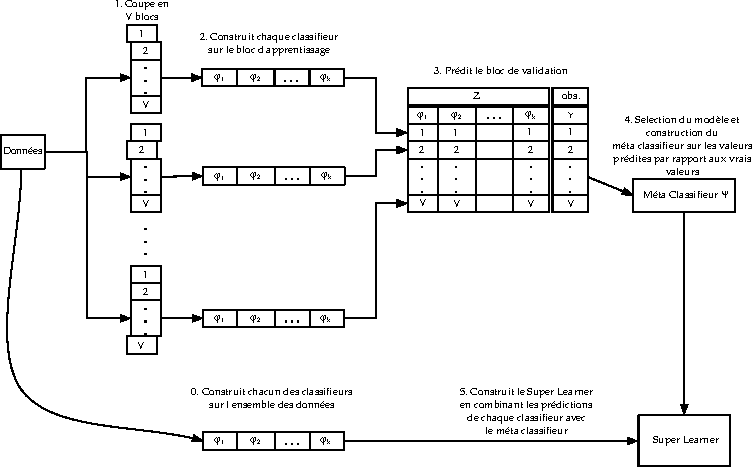
\includegraphics{Superlearner.pdf}
    }
    \caption{Fonctionnement de l'algorithme SuperLearner, adapté de \citet{VanderLaan2007a}}
\end{figure}

Le choix de l'algorithme de meta-apprentissage $\Psi$ influe également grandement sur les performances du super classifieur, il est possible de choisir une fonction aussi simple que le vote majoritaire ou la moyenne non pondérée ou arbitrairement complexe comme un réseau de neurones artificiels profond, le choix étant alors à faire en fonction de jeux de données, de la mesure de performance choisie et le temps de calcul disponible. \citet{Jahrer2010} fournit un aperçu de différentes techniques de mélange et leurs performances.

Ces méthodes de mélange considèrent tous les modèles disponibles quelque soit leur contribution aux performances, pour pallier ce problème et permettre une optimisation de l'ensemble de modèles par rapport à la métrique de son choix. \citet{Caruana2011a} proposent une méthode de construction d'ensemble par étapes où seuls les classifieurs améliorant la qualité de l'ensemble sont rajoutés. En ne prenant comme fonction de mélange que la moyenne, ils permettent des combinaisons très rapides, ce qui autorise l'utilisation de milliers de classifieurs de base. Mais il est tout à fait envisageable d'utiliser un meta classifieur plus performant.

\begin{figure}[htbp]
    \begin{tikzpicture}
    \begin{axis}[domain=0:1, ymin=0, ymax = 1, enlargelimits = false, xlabel = {Taux de faux positifs}, ylabel = {Taux de vrais positifs}, legend style={draw=none,legend pos=south east}]
            \addplot[no markers, const plot, blue] table [x = "fpr", y = "tpr", col sep = comma] {images/roc_stacking.csv};
            \addlegendentry{Stacking NN}
            \addplot[no markers, const plot] table [x = "fpr", y = "tpr", col sep = comma] {images/roc_arbre.csv};
            \addlegendentry{Arbre seul}
            \addplot[no markers, black, dashed] {x};
    \end{axis}
    \end{tikzpicture}
    \caption{Performances du stacking avec réseaux de neurones ($\mathrm{AUC} = 0.7372$).}
\end{figure}

\todo{refaire le diagramme}
\todo{donner exemple, procédure avec Echantillon Train; Echantillon Blend et Echantillon Test}
% !TEX encoding = UTF-8 Unicode
% !TEX TS-program = LuaLaTeX
% !TEX root = ../memoire.tex
% !TEX spellcheck = fr-FR

%************************************************
\chapter{Arbres et forêts}
\label{chap:quatre}
%************************************************

\section{Arbres de décision}

\todo{Trop "inspiré" de Louppe.}

La performance pure des méthodes statistiques a toujours été l'un des principaux moteurs de la recherche dans le domaine, mais cela n'est pas le seul critère de la qualité d'un modèle. En effet, l'interprétabilité d'un modèle est dans beaucoup de domaines aussi, si ce n'est plus, important que la performance du modèle. Parmi ces modèles explicatifs, l'un sort du lot par sa combinaison de bonnes performances et facilité de compréhension: les arbres de décision. Nous suivrons les notations et définitions de \citet{Louppe2014}, et renvoyons à sa thèse pour un aperçu exhaustif de la littérature existante ainsi qu'une analyse de l'implémentation et la complexité algorithmique des arbres et forêts aléatoires, ce chapitre n'a pas donc vocation a apporter un point de vu original.
Historiquement introduit par Morgan et Sonquist en 1963 la version moderne de ces arbres a été introduite indépendamment par Breiman, Friedman et Quinlan. Plus précisément c'est le modèle \ac{cart} de \citet{Breiman1984a} qui introduit de façon rigoureuse et unifiée la théorie des arbres de décision.
Avant même d'en étudier leurs caractéristiques, il est possible de donner plusieurs raisons expliquant la popularité des arbres de décision
\begin{itemize}
    \item Ils sont non-paramétriques.
    \item Ils peuvent traiter les données hétérogènes (mélange de variables qualitatives et quantitatives) ainsi que les données manquantes.
    \item Ils effectuent automatiquement une sélection des variables et sont donc en partie résistants aux variables inutiles ou bruitées.
    \item Ils sont résistants aux outliers ou erreurs d'étiquetage.
    \item Ils sont faciles d'interprétation.
\end{itemize}

\subsection{Structure}

De la façon la plus générale, on peut voir un arbre de décision comme une partition récursive de l'espace ce qui est tout particulièrement adapté aux problèmes de classification. En effet si $\mathcal{Y} = \{c_1, \dotsc, c_j \}$\label{ntn:c_k} est l'espace des classes, alors on peut voir notre problème de classification supervisée sur $\Omega$ comme une partition 
\begin{equation*}
    \Omega = \Omega_{c_1} \cup \dotsc \cup \Omega_{c_j}    
\end{equation*}
avec $\Omega_{c_k}$ l'ensemble des individus de classe $c_k$. On peut donc voir notre classifieur $\varphi$ comme une partition de l'espace puisqu'il définit une approximation $\hat{Y}$ de $Y$, à l'exception que cette partition se fait sur $\mathcal{X}$ au lieu de $\Omega$ directement. On a alors:
\begin{equation*}
    \mathcal{X} = \mathcal{X}^{\varphi}_{c_1} \cup \dotsc \cup \mathcal{X}^{\varphi}_{c_j}
\end{equation*}
où $\mathcal{X}^{\varphi}_{c_k}$ est l'ensemble des $x \in \mathcal{X}$ tels que $\varphi (x) = c_k$. Notre problème d'apprentissage peut alors se réécrire comme un problème d'approximation de la partition optimale de Bayes:
\begin{equation*}
    \mathcal{X} = \mathcal{X}^{\varphi_B}_{c_1} \cup \dotsc \cup \mathcal{X}^{\varphi_B}_{c_j}
\end{equation*}

Nous pouvons donc maintenant créer nos arbres comme des partitions récursives de l'espace.

\begin{definition}[Arbre enraciné]
    Un arbre enraciné est un graphe acyclique orienté $G=(V,E)$ où l'un des nœuds est désigné comme racine et toutes les arrêtes fuient la racine.
\end{definition}

\begin{definition}[Nœuds]
    S’il existe une arrête de $t_1$ vers $t_2$ alors $t_1$ est appelé nœud père de $t_2$ et $t_2$ nœud fils de $t_1$. 
\end{definition}

\begin{definition}
    Un nœud d'un arbre enraciné est dit interne s’il possède au moins un fils et terminal (ou feuille) sinon.
\end{definition}

\begin{definition}
    Un arbre binaire est un arbre enraciné où chaque nœud interne possède exactement $2$ fils: le fils gauche et le fils droit notés à partir d'ici respectivement $t_L$ et $t_R$.
\end{definition}

Dans ces conditions, un \emph{arbre de décision} est un classifieur $\varphi : \mathcal{X} \rightarrow \mathcal{Y}$ représenté par un arbre enraciné où chaque nœud $t$ représente un sous-espace $\mathcal{X}_t \subseteq \mathcal{X}$ avec la racine $t_0$ représentant $\mathcal{X}$ tout entier. Les fils $t_i, \dotsc, t_j$ de $t$ représentent alors une partition disjointe de $\mathcal{X}_t$. Chaque feuille est alors étiquetée avec $\hat{y}_t \in \mathcal{Y}$, la meilleure approximation possible de $y$. Si $\mathcal{Y} = \{c_1,\dotsc,c_j\}$ alors l'arbre est dit de classification, si $\mathcal{Y} = \mathbb{R}$ il est dit de régression, ce ne sont pas les seuls types d'arbres possibles et l'on peut notamment citer les arbres de quantiles \citep{Meinshausen2006}, de densités \citep{Ram2011} ou de survie \citep{Ishwaran2008}. Alors $\varphi(x)$ est l'étiquette de la feuille atteinte à partir de $t_0$ en suivant les règles de coupure. Le choix de représenter un problème de classification par un graphe acyclique est tout à fait raisonnable. En effet, on cherche à modéliser un système complexe par les interactions entre les différentes variables aléatoires qui le composent, ce qui correspond exactement au cadre général plus vaste des \emph{modèles graphiques}. Néanmoins en restreignant le type de graphe considéré on se ramène à un problème de partitionnement bien plus facile à étudier que ce soit de manière théorique ou dans la résolution pratique.

Le choix de représenter le problème sous la forme d'arbres est arbitraire et ne sert qu'à rendre les calculs plus faciles, il est tout à fait envisageable de détendre les restrictions sur la forme du graphe et autoriser par exemple plusieurs ancêtres. Les performances peuvent ainsi être améliorées au détriment de la facilité de calcul \citep{Shotton2013a}.

\begin{figure}[htbp]
    \centering
    \begin{subfigure}[b]{.45\textwidth}
    \centering    
    \begin{tikzpicture}
    % Draw axes
    \draw [<->,thick] (0,4) node (yaxis) [above] {$x_2$}
          |- (5,0) node (xaxis) [right] {$x_1$};
    % Draw line
    \draw[dashed] (2.7,0.1) -- (2.7,1.25);
    \draw[dashed] (2.7,1.25) -- (2.7,3.9);
    \draw[dashed] (0.1,1.35) -- (2.6,1.35);
    \draw[dashed] (1.5,0.1) -- (1.5,1.25);
    % Draw negative dots
    \fill[black] (0.5,1.5)   circle (3pt);
    \fill[black] (1.5,2.5)   circle (3pt);
    \fill[black] (1,2.5)     circle (3pt);
    \fill[black] (0.75,2)    circle (3pt);
    \fill[black] (0.6,1.9)   circle (3pt);
    \fill[black] (0.77, 2.5) circle (3pt);
    \fill[black] (1.5,3)     circle (3pt);
    \fill[black] (1.3,3.3)   circle (3pt);
    \fill[black] (0.6,3.2)   circle (3pt);
    \fill[black]   (2.2,1.2)   circle (3pt);
    \fill[black]   (2,1)   circle (3pt);
    \fill[black]   (2.3,0.7)   circle (3pt);
    % Draw positive dots
    \draw[black] (0.2,1.17)     circle (3pt);
    \draw[black] (0.5,0.2)     circle (3pt);
    \draw[black] (0.36,0.75)     circle (3pt);
    \draw[black] (0.9,0.8)     circle (3pt);
  
    \draw[black] (4,1)     circle (3pt); 
    \draw[black] (3.3,.3)  circle (3pt); 
    \draw[black] (4.5,1.2) circle (3pt); 
    \draw[black] (4.5,.5)  circle (3pt); 
    \draw[black] (3.9,.7)  circle (3pt); 
    \draw[black] (5,1)     circle (3pt); 
    \draw[black] (3.5,.2)  circle (3pt); 
    \draw[black] (4,.3)    circle (3pt); 
    \end{tikzpicture}
    \end{subfigure}
    ~
    \begin{subfigure}[b]{.45\textwidth}
    \centering
        \begin{forest}
        [$x_1 \leq 2.7$
            [$x_2 \leq 1.35$
                    [$x_1 \leq 1.5$
                        [,circle, draw]
                        [,circle, fill]
                    ]
                [,circle, fill]
            ]
            [,circle, draw]
        ]       
    \end{forest}
    \end{subfigure}
    \caption{Équivalence entre la partition du plan et un arbre de décision binaire}
\end{figure}

\subsection{Critère d'impureté}

Apprendre un arbre de décision revient alors à déterminer la plus petite des partitions la plus proche de la partition engendrée par $Y$ sur $\mathcal{X}$, ce problème est en réalité NP-complet et trouver la meilleure approximation est impossible en un temps raisonnable. Il est donc nécessaire de développer une heuristique permettant de construire l'arbre par induction en maximisant une fonction "objectif" assurant de faire un choix judicieux à chaque étape. Ainsi \citet{Breiman1984a} définissent une notion de mesure d'\emph{impureté} $i(t)$ qui évalue la qualité de la partition courante en $t$. Dans ce cadre, plus $i(t)$ est petit, plus le nœud est \emph{pur} et meilleure est la prédiction $\hat{y}_t (x)$, où $(x,y) \in \mathcal{L}_t$ avec
\begin{equation*}
    \mathcal{L}_t = \left \{ (x,y) \in \mathcal{L} \mid x \in \mathcal{X}_t \right\}    
\end{equation*}
et $\mathcal{X}_t$ le sous-ensemble de l'espace représenté par le nœud $t$ (donc $\mathcal{X}_{t'} \subset \mathcal{X}_t$ si $t'$ est un descendant de $t$ et $\mathcal{X} = \bigcup \mathcal{X}_t$).

On obtient ainsi tout naturellement un algorithme glouton de construction de l'arbre: en partant d'une racine représentant l'ensemble d'apprentissages tout entier (et donc l'espace tout entier) chaque itération divise la population du nœud courant de façon à minimiser l'impureté des nouveaux nœuds, l'algorithme s'arrête lorsque l'impureté ne peut plus être réduite.
Définissons alors la diminution de l'impureté pour une coupure binaire $s$ en $t$:

\begin{definition}
    La \emph{réduction d'impureté pondérée} d'une partition binaire $s \in \mathcal{Q}$ divisant $t$ en $t_L$ et $t_R$ est:
    \begin{equation*}
        \Delta i(s,t) = i(t) - p_L i(t_L) - p_R i(t_R)
    \end{equation*}
    où $p_L$ (resp. $p_R$) est le rapport $\frac{N_{t_L}}{N_t}$ (resp. $\frac{N_{t_R}}{N_t}$) d'échantillons d'apprentissage de $\mathcal{L}_t$ allant dans $t_L$ (resp. $t_R$) avec $N_t = \vert \mathcal{L}_t \vert$
\end{definition}

\subsubsection{Classification}

Dans le cas de la classification, le rôle de l'arbre est la minimisation de l'erreur de généralisation. Il peut donc sembler naturel de prendre pour $i(t)$ l'estimation locale de la certitude de classification en $t$.

\begin{definition}
    Dans le cas de la classification, l'\emph{impureté} $i_R (t)$ basée sur l'estimation locale de la certitude de classification définie sur la perte $0$-$1$ est:
    \begin{equation*}
        i_R (t) = 1 - p(\hat{y}_t \mid t ) = 1 - \max_{c \in \mathcal{Y}} p(c\mid t)
    \end{equation*}
\end{definition}
Ce choix est naturel puisqu’il revient à choisir la coupure qui minimise l'erreur d'apprentissage. Néanmoins cette notion d'impureté a plusieurs défauts:
\begin{enumerate}
    \item $\Delta i(s,t)$ vaut $0$ pour toutes les coupures pour lesquelles tous les fils gardent la même classe majoritaire, c'est-à-dire si $y_t = y_{t_L} = y_{t_R}$. Toutes les coupures sont alors considérées comme aussi bonnes.
    \item Il y a peu d'impact de la distribution a posteriori des classes $p(y\mid t_L)$ et $p(y\mid t_R)$.
\end{enumerate}
Ces défauts sont principalement dus au processus de création de l'arbre: puisque l'arbre est construit de manière gloutonne, il faudrait que notre notion d'impureté prenne en compte les possibilités de réduction future de l'impureté dans les étapes suivantes. Pour éviter les défauts de $i_R (t)$ le choix de $i(t)$ doit être fait de telle sorte que celui-ci décroît au fur et à mesure que les nœuds $t$ deviennent plus homogènes. Dans l'algorithme \ac{cart}, \citet{Breiman1984a} identifient une famille de fonctions d'impureté $i(t)$ qui répond à ce critère:
\begin{theoreme}
\label{impurete}
    Soit $\Phi (p_1,\dotsc,p_J)$ une fonction strictement concave définie sur $0 \leq p_k \leq 1$, pour $k=1,\dotsc,J$ et $\sum_{k=1}^J p_k = 1$ telle que:
    \begin{itemize}
        \item $\Phi (1,\dotsc,0) = \Phi (0,1,\dotsc,0) = \dots = \Phi ( 0,\dotsc,1)$ soit minimale
        \item $\Phi \left(\frac{1}{J},\dotsc,\frac{1}{J} \right)$ soit maximale
    \end{itemize}
    Alors pour $i(t) := \Phi \left( p(c_1 \mid t), \dotsc, p(c_J \mid t) \right)$ et pour n'importe lequel $s$,
    \begin{equation*}
        \Delta i(s,t) \geq 0
    \end{equation*}
    avec égalité si et seulement si $p(c_k \mid t_L) = p(c_k \mid t_R) = p(c_k \mid t)$ pour $k=1,\dotsc,J$
\end{theoreme}
Les critères d'impuretés les plus courants dans le cas des arbres de classifications sont l'entropie de Shannon et l'indice de Gini:
\begin{definition}
    La fonction d'impureté $i_H (t)$ basée sur l'entropie de Shannon \citep{Shannon1957} est:
    \begin{equation*}
        i_H (t) = - \frac{1}{2} \sum_{k=1}^J p(c_k \mid t) \log_2 \left( p(c_k \mid t ) \right)
    \end{equation*}
\end{definition}
\begin{definition}
    La fonction d'impureté $i_G (t)$ basée sur l'indice de Gini est:
    \begin{equation*}
        i_G (t) = \sum_{k=1}^J p\left(c_k \mid t \right) \left( 1-p(c_k \mid t) \right)
    \end{equation*}
\end{definition}

\begin{figure}[htbp]
    \centering
    \begin{tikzpicture}
    \begin{axis}[domain=0:1, ymin=0, ymax = 0.5, enlargelimits = false, legend style={draw=none},cycle list name=color]
        \addplot+[no markers, smooth] { 2* x * (1-x) };
        \addlegendentry{$i_G (t)$}
        \addplot+[no markers, smooth] { 1/2*(- x * log2(x) - (1-x)*log2(1-x)) };
        \addlegendentry{$i_H (t)$}
        \addplot+[no markers] { 1 - max(x,1-x) };
        \addlegendentry{$i_R (t)$}
    \end{axis}
    \end{tikzpicture}
    \caption{Comparaison de $i_R$, $i_H$ et $i_G$}
\end{figure}

$i_H$ et $i_R$ répondent toutes les deux aux conditions du théorème~\ref{impurete} mais représentent des quantités différentes. $i_H$ qui est basée sur l'entropie mesure l'incertitude de $Y$ en $t$, avec ce critère d'impureté $\Delta i_H (s,t)$ qu'on appellera alors \emph{gain d'information}. Il représente l'information apprise sur $Y$ en coupant $t$ en $t_L$ et $t_R$. L'impureté de Gini $i_G$ mesure quant à elle avec quelle fréquence un objet $x \in \mathcal{L}_t$ choisi au hasard serait incorrectement classifié s'il était étiqueté par $c \in \mathcal{Y}$ au hasard suivant la loi $p(y \mid t)$. Ces deux notions d'impureté ne sont pourtant pas parfaites, en effet elles présentent toutes les deux la propriété dite \ac{ecp} qui peut rendre un arbre profond et donc difficilement interprétable. De plus les coupes sont biaisées vers la variable possédant le plus de réalisations. De nombreuses alternatives de critères d'impureté existent pour tenter de remédier à ces problèmes telles que le \emph{ratio de gain d'information} utilisé dans les \ac{et}, mais les changements dans la structure de l'arbre induits par le choix de la mesure d'impureté n'ont en réalité que peu d'impact sur la performance en terme de classification \citep{Louppe2014}.

\subsubsection{Régression}

Dans le cas de la régression, c'est-à-dire quand la variable $Y$ est quantitative, il est possible de tout simplement choisir l'erreur $L^2$ locale sans rencontrer les problèmes du cas de la classification.

\begin{definition}
    En régression, la mesure d'impureté $i_R (t)$ issue de l'estimation locale de l'erreur $L^2$ est définie par:
    \begin{equation*}
        i_R (t) = \frac{1}{N_t} \sum_{x,y \in \mathcal{L}_t} (y-\hat{y}_t)^2
    \end{equation*}
\end{definition}
Cela revient donc à minimiser la variance de chacun des noeuds. Il est intéressant de remarquer que le problème de classification binaire avec critère de Gini est en réalité strictement équivalent à un problème de régression avec erreur $L^2$. En effet puisque $\hat{y}_t = \frac{1}{N_t} \sum_{x,y \in \mathcal{L}_t} y = p(c_2 \mid t) = 1 - p(c_1 \mid t)$ on a:
\begin{align*}
    i_R (t) &= \frac{1}{N_t} \sum_{x,y \in \mathcal{L}_t} (y-\hat{y}_t)^2 \\
            &= \hat{y}_t - 2 \hat{y}_t^2 + \hat{y}_t^2 \\
            &= \hat{y}_t (1 - \hat{y}_t) \\
            &= p(c_2 \mid t) (1-p(c_2 \mid t)) \\
            &= \frac{1}{2} i_G (t)
\end{align*}

\subsection{Sélection du point de coupe}

\subsubsection{Familles $\mathcal{Q}$ de règles de partition}

Comme vu précédemment une coupure $s$ du nœud $t$ est une partition disjointe de $\mathcal{X}_t$ où chaque partie disjointe correspond à l'un des fils de $t$. Dans le cas où $s$ partitionne en deux parties disjointes on appelle $s$ une coupure \emph{binaire} de fils $t_L$ et $t_R$, cependant dans le cas plus général, $s$ peut partitionner $\mathcal{X}_t$ en $N$ avec tout autant de fils.
L'ensemble $S$ de toutes les coupures $s$ est l'ensemble de toutes les partitions disjointes de $\mathcal{X}_t$, qui est de cardinal infini dès que les variables peuvent prendre un nombre infini de valeurs, néanmoins il n'est utile de considérer que les partitions qui engendrent une partition de $\mathcal{L}_t$ de parties non vides. Ainsi dans le cadre de l'apprentissage, le problème de trouver la meilleure coupure $s^*$ de $\mathcal{X}_t$ se résume à trouver la meilleure partition du sous-échantillon d'apprentissage $\mathcal{L}_t$. Si l'on considère que les $N_t$ échantillons d'apprentissage sont distincts, le nombre de partitions de $\mathcal{L}_t$ en $k$ sous-ensembles non vides est donné par \citet{Knuth1992}:
\begin{equation*}
    S(N_t,k) = \frac{1}{k!} \sum_{j=0}^k (-1)^{k-j} \binom{k}{j} k^{N_t}
\end{equation*}
qui vaut $2^{N_t-1}-1$ pour une partition binaire. Il est clair que tester naïvement toutes les coupures possibles et ne garder que la meilleure est impossible. Nous allons donc effectuer des hypothèses limitantes sur $s^*$ c'est-à-dire chercher $s^*$ dans une famille $\mathcal{Q} \subseteq \mathcal{S}$ de coupures possibles qui donne toujours une approximation suffisamment bonne de la partition optimale.
Le choix habituel naturel pour $\mathcal{Q}$ est la famille des coupures binaires définies sur une variable unique et sans sous-ensembles vides:
\begin{equation*}
    \mathcal{Q} = \left\{ s \mid \bigcup_{j=1}^p \mathcal{Q}(X_j) , \mathcal{L}_{t_L} \neq \emptyset, \mathcal{L}_{t_R} \neq \emptyset \right\}
\end{equation*}
\begin{itemize}
    \item Si $X_j$ est une variable ordonnée à valeurs dans $\mathcal{X}_j$ alors l'ensemble des coupures binaires sur $X_j$ est: 
    \begin{equation*}
        \mathcal{Q}(X_j) = \left\{ \left( \left\{ x \mid x_j \leq \nu \right\},\left\{ x \mid x_j \geq \nu \right\} \right)  \mid \nu \in \mathcal{X}_j \right\}
    \end{equation*}
    Il s'agit géométriquement de partitions de $\mathcal{X}$ à l'aide d'hyperplans parallèles aux axes.
    \item Si $X_j$ est une variable catégorielle non ordonnée à valeurs dans $\mathcal{X}_j = \{b_1,\dotsc,b_L\}$\label{ntn:b_l} alors on prend pour $\mathcal{Q}(X_j)$:
    \begin{equation*}
        \mathcal{Q}(X_j) = \left\{ \left( \left\{ x \mid x_j \in \mathcal{B} \right\},\left\{ x \mid x_j \in \overline{\mathcal{B}} \right\} \right)  \mid \mathcal{Q} \subset \{ b_1,\dotsc,b_L \} \} \right\}
    \end{equation*}
\end{itemize}
Notre problème de minimisation de l'\emph{impureté} est alors:
\begin{equation*}
\begin{cases}
    s^* = \operatornamewithlimits{argmax}\limits_{ \substack{s_j^* \\ j=1,\dotsc,p}} \Delta i(s^*_j,t) \\
    s^*_j = \operatornamewithlimits{argmax}\limits_{\substack{s \in \mathcal{Q}(X_j) \\ \mathcal{L}_{t_L},\mathcal{L}_{t_R} \neq \emptyset}} \Delta i(s,t)
\end{cases}
\end{equation*}
Bien que le type de partition donné précédemment soit le plus couramment utilisé et celui adopté par Breiman dans les forêts aléatoires classiques et leurs variantes, on notera qu'il n'est pas nécessaire de se restreindre à des hyperplans parallèles aux axes et alors opter pour des coupures dites obliques. On peut même éventuellement utiliser des surfaces de décision non linéaires ou lever la restriction sur le caractère disjoint de la partition.

\subsubsection{Recherche de la coupure binaire optimale}\label{subsubsec:coupure_binaire}

\todo{Mieux expliquer}

Maintenant que le problème d'optimisation est bien défini, il convient de trouver le point de coupure optimal. Il faut alors faire la distinction entre les variables ordonnées et catégorielles. \citet{Louppe2014} propose un algorithme pour chacun des cas afin de simplifier la recherche du point de coupure optimal dans la majorité des cas.

Dans le cas d'une variable ordonnée, il remarque en effet qu'il est possible de calculer $\Delta i(s_j^{\nu'_{k+1}},t)$ à partir de $\Delta i(s_j^{\nu'_{k}},t)$ où $\{ \nu'_{k} \}$ est la famille des points de coupure potentiels ordonnés que l'on choisit comme étant les réalisations dans le cas où $\mathcal{X}_{j}$ est discret et le point médian entre les réalisations dans le cas où $\mathcal{X}_{j}$ est continue.

Dans le cas d'une variable catégorielle et pour la classification binaire une approche naïve forcerait à évaluer $2^{L-1}-1$ partitions, mais \citet{Breiman1984a} prouvent le théorème suivant permettant de se ramener à $L-1$ partitions:

\begin{theoreme}
\label{partition:categ}
    Quitte à réordonner les $X_j$ tel que:
    \begin{equation*}
        p(c_1 \mid t , X_j = b_{l_1} ) \leq p(c_1 \mid t , X_j = b_{l_2} ) \leq \dots \leq p(c_1 \mid t , X_j = b_{l_L} )
    \end{equation*}
    Si $i(t)$ est tel que dans le théorème~\ref{impurete} alors une des $L-1$ sous-parties $\mathcal{B} = \{b_{l_1},\dotsc,b_{l_h} \} $, $h=1,\dotsc,L-1$ définit une partition binaire de l'échantillon du nœud en:
    \begin{align*}
        &\mathcal{L}^{\mathcal{B}}_{t_L} = \{ (x,y) \mid (x,y) \in \mathcal{L}_{t} ,x_j \in \mathcal{B} \} \\
        &\mathcal{L}^{\mathcal{B}}_{t_R} = \{ (x,y) \mid (x,y) \in \mathcal{L}_{t} ,x_j \in \overbar{\mathcal{B}} \}
    \end{align*}
\end{theoreme}
On traite alors $X_j$ comme une variable ordonnée en remplaçant les $b_l$ par $p(c_1 \mid t , X_j = b_{l})$. Malheureusement le théorème~\ref{partition:categ} ne s'étend pas au cas de la classification multiclasse où la seule solution reste d'évaluer les $2^{L-1}-1$ partitions ou, à défaut, un sous-ensemble aléatoire.

\todo{Algo 3.4}

\subsubsection{Coupures aléatoires et \ac{ecp}}

La recherche du point de coupure aléatoire est très chère et le gain apporté par un choix optimal dépend fortement de la régularité de la fonction que l'on cherche à approcher, des caractéristiques de la fonction d'impureté choisie et des caractéristiques de l'espace d'apprentissage $\mathcal{X}$. Au vu de la difficulté de s'assurer que couper de façon optimale apporte un quelconque gain, il peut sembler judicieux d'économiser du temps de calcul en coupant de manière aléatoire.
Il est possible de réduire l'espace de recherche de deux façons:
\begin{itemize}
    \item En ne considérant qu'un sous-ensemble choisi aléatoirement de variables à considérer. Il s'agit de la méthode \ac{rs} introduite par \citet{Ho1998}
    \item En choisissant parmi un ensemble de points de coupures tirés aléatoirement
\end{itemize}
Ces techniques de randomisation sont d'une grande importance pour la construction des forêts aléatoires comme nous le verrons ensuite, on peut donc donner quelques exemples d'arbres aléatoires

\begin{description}
    \item[\ac{extra}]
    Introduits par \citet{Geurts2006}, ici à chaque nœud $K$ variables sont choisies aléatoirement et $K$ points de coupures sont tirés uniformément parmi l'ensemble des valeurs réalisées de chacune de ces variables, la coupure qui minimise l'impureté est alors choisie.
    \item[\ac{UBPRF}]
    Introduit par \citet{Breiman2001} pour ses caractéristiques théoriques, ici on choisit aléatoirement le nœud à partitionner, puis on choisit aléatoirement la variable de coupure et enfin le point de coupure est choisi aléatoirement parmi les réalisations.
    \item[\ac{pert}]
    Dans cette construction de \citet{Cutler2001} il n'y a plus de critère de réduction de l'impureté; à chaque nœud $2$ individus $x_{1,j}$ et $x_{2,j}$ sont tirés aléatoirement de façon à ce qu'ils soient d'une classe différente, puis une variable de coupure est tirée elle aussi aléatoirement. La dernière étape consiste à tirer uniformément sur $[x_{1,j},x_{2,j}]$ un point de coupure. La procédure de construction de l'arbre s'arrête lorsque tous les nœuds actuels sont purs.
    \item[Arbres uniformément aléatoires] 
    Ici \citet{Ciss2013} tire $\lceil \beta d \rceil$ variables avec remise ($\beta > 0$) puis les points de coupures sont choisis uniformément sur le support de $X_j$. Le critère de maximisation de la réduction d'impureté est ici utilisé comme précédemment.
\end{description}

Comme nous le verrons plus tard ces arbres aléatoires sont importants pour la création de forêts aléatoires et présentent souvent de bonnes performances pratiques en évitant les éventuelles caractéristiques problématiques des données. Néanmoins \citet{Ishwaran2014} montre que, du moins dans certains cas, les coupures aléatoires sont moins bonnes que celles vues précédemment. Commençons tout d'abord par introduire la notion de variable de bruit et de propriété \ac{ecp}.

\begin{definition}
    Si $X$ est la caractéristique à $p$ dimensions et $Y$ la variable à prédire on appelle \emph{variable bruyante} une variable $X_j \subseteq \mathcal{X}$ si la loi conditionnelle de $Y$ sachant $X$ est indépendante de $X_j$. Elle est appelée \emph{variable forte} dans le cas contraire.
\end{definition}

\begin{definition}
    Une règle de coupure a la propriété \ac{ecp} si elle tend à couper aux bords pour les variables bruyantes. C'est-à-dire si $\hat{s}_N$ est le point de coupure optimal parmi les points de coupures possibles $x_1 \leq \dotsc \leq x_N$ alors si $X_j$ est bruyante $\hat{s}_N$ tend vers $x_1$ ou $x_N$.
\end{definition}

La propriété \ac{ecp} a longtemps été considérée comme indésirable, car ayant tendance à provoquer des arbres très profonds, mais selon Ishwaran celle-ci est en réalité bénéfique puisqu’en coupant aux bords pour les variables bruyantes on ne dilue pas l'échantillon pour des coupures inutiles et il sera possible de recouper sur des variables fortes plus profondément dans l'arbre.

On peut de plus calculer le point de coupure optimal en fonction de la fonction à estimer $f$ ($Y = f(x) + \varepsilon$) dans le cadre d'une population de nœuds infinie.

\begin{theoreme}
    Soit $\varphi (s) = \mathbb{P} [Y = 1 \mid X = s]$. Si $\varphi (s)$ est continu sur $t = [a,b]$ et $\mathbb{P}$ admet une densité continue positive sur $t$ alors la coupure $s$ optimale au sens de la réduction de l'impureté de Gini dans le cas de la classification binaire est solution de
    \begin{equation}
        2 \varphi (s) = \int_a^s \varphi (x) \mathbb{P}_{t_L} (\diff x) + \int_s^b \varphi (x) \mathbb{P}_{t_R} (\diff x) , a \leq s \leq b
    \end{equation}
\end{theoreme}

\begin{theoreme}
    Le processus de coupure basé sur l'impureté de Gini a la propriété \ac{ecp}.
\end{theoreme}

%\begin{proof}
    \todo{Gini ECP preuve ?}
%\end{proof}

\subsection{Critère d'arrêt}

Plus un arbre de décision est profond, plus son erreur d'apprentissage est faible, mais l'erreur d'apprentissage ne reflète pas forcément l'erreur de généralisation, c'est-à-dire l'erreur sur un échantillon de taille infinie distribué selon la vraie distribution des individus. En effet, un tel arbre a tendance à surapprendre (\emph{overfitting}) et à capturer le bruit plus que l'information. Il est alors nécessaire de trouver un compromis entre sur et sous-apprentissage et donc entre un arbre trop peu profond (l'extrême étant un arbre de profondeur $1$, aussi appelé \emph{souche de décision}) et un arbre trop profond qui obtiendrait alors des performances parfaites sur l'échantillon d'apprentissage et très mauvaises sur l'échantillon test.

\missingfigure{Tradeoff sur/sous apprentissage}

\begin{figure}[htbp]
    \begin{tikzpicture}
    \begin{axis}[ymin=0, ymax = 0.5, enlargelimits = false, xlabel = {Degrés du polynome}, ylabel = {Taux d'erreur}, legend style={draw=none,legend pos=north west}]
            \addplot[no markers, blue] table [x = "i", y = "train", col sep = comma] {images/sursousapp.csv};
            \addlegendentry{Apprentissage}
            \addplot[no markers] table [x = "i", y = "val", col sep = comma] {images/sursousapp.csv};
            \addlegendentry{Validation}
    \end{axis}
    \end{tikzpicture}
    \caption{Sur-apprentissage dans le problème d'apprentissage de $sin(x)$~\ref{fig:biaisvar}}
\end{figure}

Il est donc nécessaire d'avoir une règle d'arrêt de la procédure de coupe récursive. Notons tout d'abord que la procédure de partition possède deux critères d'arrêt inhérents à la procédure:
\begin{enumerate}
    \item lorsque $\mathcal{L}_t$ est homogène, c'est-à-dire que tous les individus ont la même étiquette
    \item lorsque les variables de tous les individus de $\mathcal{L}_t$ sont identiques
\end{enumerate}
Pour empêcher le sur-apprentissage un certain nombre de critères d'arrêt heuristiques peuvent être ajoutés:
\begin{enumerate}
    \item Fixer une taille $N_{\text{min}}$ de l'échantillon pour la partition.
    \item Fixer une profondeur $d_{\text{max}}$ de l'arbre.
    \item Fixer une réduction $\beta$ minimum de l'impureté.
    \item Fixer une taille $N_{\text{feuille}}$ minimum pour chacun des fils en cas de coupure.
\end{enumerate}

Toutes ces variables forment un jeu d'hyper-paramètres qu'il est possible d'optimiser pour obtenir les performances désirées.

\subsection{Importance des variables}

Bien que le but principal d'un algorithme de classification supervisée soit l'étiquetage de nouveaux individus en fonctions de leurs variables, une question naturelle et très importante dans de nombreux domaines comme la bio-informatique est la question de l'importance des variables. Mesurer l'importance des variables dans l'explication du facteur à prédire fournit ainsi une forme d'explication du mécanisme régissant ce facteur. Les arbres aléatoires sont facilement interprétables et il est donc possible d'établir plusieurs mesures de l'importance des variables.

\subsubsection{Diminution de l'impureté}

L'importance de $X_j$ par diminution de l'impureté dans le cas d'un arbre seul est introduite par \citet{Breiman1984a} comme la diminution totale de l'impureté si l'on effectuait les coupures uniquement sur $X_j$ à chaque nœud en imitant la coupure réelle au mieux possible.
C'est-à-dire
\begin{equation*}
    \operatorname{Imp}(X_j) = \sum_{t \in \varphi} \Delta I(\tilde{s}_t^j,t)
\end{equation*}
ou $\tilde{s}_t^j$ est la coupure suppléante en $t$ sur $X_j$, c'est à dire la coupure qui minimise la distance entre les distributions des classes dans les noeuds fils. On remplace toutes les coupures de l'arbre par leur coupure suppléante sur $X_j$ de façon à minimiser les effets de masquage. En effet une variable peut être importante, mais toujours donner une diminution de l'impureté légèrement inférieure aux autres, cette variable ne sera alors jamais sélectionnée et apparaîtrait comme d'importance nulle.

\todo{Donner une formule explicite. EMD ?}

\subsubsection{Diminution de l'erreur}

Il est également possible de mesurer l'importance d'une variable en mesurant sa contribution à la précision de la prédiction. Pour cela on permute les valeurs des observations de la variable $X_j$ d'intérêt, et l'on mesure la diminution de la précision.
\begin{align*}
    \operatorname{Imp}(X_j) &= \frac{1}{N} \sum_{(x'_i,y_i) \in \pi_j(\mathcal{L})} \mathds{1}_{\varphi(x'_i) \neq y_i} \\
    &- \frac{1}{N} \sum_{(x_i,y_i) \in \mathcal{L}} \mathds{1}_{\varphi(x_i) \neq y_i}
\end{align*}
où $\pi_j(\mathcal{L})$ est $\mathcal{L}$ où l'on a permuté les valeurs de $X_j$.
Si $X_j$ est une variable prédictive alors on s'attend à ce que changer ses valeurs détériore le pouvoir prédictif de la forêt.

\subsubsection{Profondeur minimale}

Dans \citet{Ishwaran2007}, l'auteur introduit la notion de $v$ sous-arbre maximal pour étudier les propriétés théoriques de l'importance des variables par diminution de l'impureté. Un $v$ sous-arbre est un sous-arbre dont la racine définit une coupe selon la variable $v$, il est maximal s’il n'est pas lui même $v$ sous-arbre d'un autre $v$ sous-arbre.
Dans \citet{Ishwaran2010a} les auteurs utilisent cette notion de sous arbre pour définir une nouvelle importance de la variable $v$ comme étant la profondeur minimale des $v$ sous-arbres de l'arbre. Il est alors possible de définir l'équivalent pour les forêts en prenant comme importance pour $v$ la profondeur minimale moyenne des $v$ sous-arbres dans la forêt.

Les variables importantes ayant une plus grande chance d'être retenues parmi les différentes variables considérées aléatoirement, on s'attend à ce que les variables importantes soient tirées tôt, les variables peu importantes n'étant tirées qu'en présence uniquement de variables moins importantes, ce qui devrait se produire peu souvent et donc n'arriver en moyenne que profondément dans l'arbre.

\todo{voir \citet{Ishwaran2010a}}

\subsection{Effeuillage}

Afin d'éviter le sur-apprentissage il est essentiel de limiter la complexité de l'arbre. En effet il est trivial en développant l'arbre jusqu'à avoir des feuilles ne comportant qu'un seul individu d'obtenir une erreur nulle sur l'échantillon d'apprentissage. Pour autant l'erreur sur l'échantillon de test explosera.
On a précédemment introduit des critères d'arrêts qui permettent d'éviter ce sur-apprentissage durant la procédure de création de l'arbre mais il est également possible d'effectuer la réduction de la complexité une fois l'arbre entièrement construit.

On procède alors à un \emph{effeuillage} de l'arbre, c'est à dire la suppression des feuilles considérées comme contribuant au sur-apprentissage.

\begin{remark}{Comparaison de différentes méthodes}
    La procédure d'effeuillage n'est pas nécéssaire dans le cas des forêts aléatoires, nous n'exposerons donc ici que une seule méthode possible afin de donner une idée mais il existe d'autres méthodes possibles. Nous renvoyons à \citet{Mingers1989} pour une comparaison des méthodes d'effeuillage d'arbres de décisions seuls.
\end{remark}

Puisque l'on cherche à trouver un compromis entre erreur et complexité, si l'on considère que le nombre de feuilles reflète la complexité d'un arbre alors \citet{Breiman1984a} propose l'algorithme d'\emph{effeuillage coût-complexité}.
On définit par $\left( \varphi_m \right)$ l'ensemble des sous-arbres de $\varphi$, ou un sous-arbre est un arbre obtenu par effeuillage successif de $\varphi$. On cherche alors:
\begin{equation*}
    \argmin_{\varphi_m} \frac{\mathrm{Err} \left[ \varphi_m , \mathcal{L}' \right] - \mathrm{Err} \left[ \varphi , \mathcal{L}' \right] }{\vert \varphi_m \vert_F - \vert \varphi \vert_F}
\end{equation*}
avec $\mathcal{L}'$ un échantillon de test et $\vert \varphi_m \vert_F$ le nombre de feuilles de $\varphi_m$.

\subsection{Consistance}

Bien que de nombreuses variantes des arbres (et par extension forêts) aléatoires sont introduites et étudiées expérimentalement, la théorie permettant d'expliquer les performances est très faible.
Le problème principal est la preuve de la consistance des arbres aléatoires de Breiman.

La consistance des arbres aléatoires est due à \citet{Biau2008,Devroye1997} et se base sur le théorème suivant:

\begin{theoreme}[\citet{Devroye1997}, page 94, théorème 6.1]
    Soit une règle de partionnement telle que:
    \begin{equation*}
        \varphi_n (\mathbf{x}) = \begin{cases}
            0 \text{ si } \sum_{i=1}^n \mathds{1}_{y_i = 1} \mathds{1}_{\mathbf{x}_i \in \mathcal{X}^\varphi (\mathbf{x})} \leq \sum_{i=1}^n \mathds{1}_{y_i = 0} \mathds{1}_{\mathbf{x}_i \in \mathcal{X}^\varphi (\mathbf{x})} \\
            1 \text{ sinon.}
        \end{cases}
    \end{equation*}
    Avec $\mathcal{X} = \bigcup \mathcal{X}^\varphi (x_i)$ la partition (finie) de l'espace définie par le classifieur.
    Notons aussi
    \begin{align*}
        N(\mathbf{x}) = \sum_{i=1}^n \mathds{1}_{\mathbf{x}_i \in \mathcal{X}^\varphi (\mathbf{x})}
    \end{align*}
    le nombre de voisins de $x$, et:
    \begin{equation*}
        \mathrm{diam} ( \mathcal{X}^\varphi ) = \sup_{x,y \in \mathcal{X}^\varphi} \Vert x - y \Vert
    \end{equation*}
    Alors $\mathrm{Err}_n ( \varphi_n ) \to  \mathrm{Err} ( \varphi_B ) $ si 
    \begin{align*}
        &\mathrm{diam} ( \mathcal{X}^\varphi (\mathbf{x}) ) \xrightarrow{\mathbb{P}} 0 \\
        &N ( \mathbf{x} ) \xrightarrow{\mathbb{P}} +\infty
    \end{align*}
\end{theoreme}

\todo{Peut on mettre le theoreme/preuve? Dans le cas Purement aléatoire par exemple???}

\section{Forêts aléatoires}

On a vu dans le chapitre~\ref{chap:trois} comment la création d'ensembles de classifieurs à forte variance permet la construction d'un ensemble de classifieurs de meilleure qualité. Les arbres de classification sont un candidat idéal pour les méthodes ensemblistes grâce à leur capacité à modéliser des relations non linéaires complexes, leurs faibles biais et dans le cas des arbres non effeuillés leur instabilité très élevée. Nous avons également vu qu'il existait plusieurs méthodes pour construire de tels ensembles, néanmoins la plus grande partie des travaux sur les forêts aléatoires porte sur des variantes de la méthode proposée par \citet{Breiman2001}. Nous regrouperons alors toutes ces méthodes sous le terme de Forêts de Breiman.

\begin{remark}{Plus de littérature}
Durant la rédaction de ce rapport un résumé de la littérature sur les forêts aléatoires par \citet{Biau2015} est apparu. Plusieurs autres méthodes sont abordées et les aspects théoriques en particulier font l'objet d'une grande attention. Le rapport technique de \citet{Criminisi2012} porte lui plus sur les aspects pratiques des forêts aléatoires, mais donne un aperçu intéressant des très nombreux problèmes pouvant être résolus par l'apprentissage machine en général et les forêts aléatoires en particulier.
\end{remark}

\subsection{Forêts de Breiman et dérivés}

On a vu dans~\ref{subsec:combinaison_lineaire} que la combinaison linéaire de classifieurs faiblement corrélés permettait la création d'un nouveau classifieur plus puissant. Il est donc nécessaire de construire une famille d'arbres aléatoires les moins corrélés possible avant d'envisager la construction de l'ensemble en lui-même. 

La première façon, dite des \ac{rs}, d'introduire de l'aléa a été introduite par \citet{Ho1998}, elle consiste à chaque étape de création d'une coupure, à tirer aléatoirement un sous-ensemble de $K$ variables de $\mathcal{X}$ puis à appliquer la procédure de choix de la coupe. Le bénéfice de cette technique est double: d'une part en introduisant de l'aléa les arbres sont en partie décorrélés, et d'autre part la réduction du nombre de coupures à considérer accélère grandement la construction de l'arbre.
Néanmoins les arbres restent fortement corrélés et pour pallier ce problème \citet{Breiman1996} introduit le \ac{bagging}. Un échantillon bootstrap de l'échantillon d'apprentissage est tiré avec remise et l'arbre est construit sur ce nouvel échantillon tiré aléatoirement. Ici encore, l'ajout d'aléa permet de décorréler les arbres et de réduire la complexité de construction des arbres d'environ $1/3$ en moyenne. Une autre des propriétés importantes issues de cette technique est l'existence d'un échantillon \ac{oob}. En effet la procédure de tirage avec remise induit qu'en moyenne $1-\left(1-\frac{1}{n}\right)^n \approx 63\% $ des observations sont utilisées pour construire chaque arbre, il est donc possible de mesurer l'erreur \ac{oob} comme approximation de l'erreur de généralisation.

\begin{definition}[Erreur \ac{oob}]
    On appelle erreur \ac{oob}:
    \begin{equation*}
        \hat{\operatorname{Err}}^{\text{OOB}} ( \psi_{\mathcal{L}} ) = \frac{1}{N} \sum_{(x_i,y_i) \in \mathcal{L}} \left( \frac{1}{M^{-i}} \sum_{l=1}^{M^{-i}} \mathds{1}_{\varphi_{\mathcal{L}^{m_{k_l}}} (x_i) \neq y_i} \right)
    \end{equation*}
    ou $m_{k_1},...,m_{k_{M^{-i}}}$ sont les $M^{-i}$ arbres construits à partir d'échantillons bootstrap ne contenant pas $(x_i,y_i)$
\end{definition}

Cette approximation de l'erreur de généralisation est au moins aussi bonne que celle obtenue par $k$-validation croisée \citep{Wolpert1999} tout en étant bien moins coûteuse numériquement.

La version de Breiman possède un bon compromis entre biais et variance et a montré de façon empirique d'excellents résultats sur un grand nombre de problèmes aussi bien artificiels que réels \citep{Fernandez-Delgado2014a}. 

Le caractère guidé, c'est-à-dire la procédure d'optimisation du point du coupe, et le choix de la meilleure coupe parmi $K$ coupes donne aux forêts aléatoires une propriété intéressante qui peut expliquer en partie les très bonnes performances observées, notamment dans le cas des grandes dimensions. En effet \cite{Breiman2004a} montre que la convergence des forêts aléatoires ne dépend que des variables dites \emph{fortes} et non pas les variables \emph{faibles} bruitées. Il montre que la convergence pour une version simplifiée des forêts aléatoires vers l'erreur de Bayes est de l'ordre de
\begin{equation*}
    N^{- \frac{3}{4 \vert S \vert + 3}}
\end{equation*}
avec $S$ les variables fortes définies telles que $\mathbb{E} \left[ y \mid \mathbf{x} \right]$ ne dépend que de $S$. Ce résulat se retrouve pour d'autre types de forêts \citep{Biau2010a} et semble donc se généraliser.

Il existe néanmoins un certain nombre de jeux de données pour lesquels le caractère guidé de l'algorithme \ac{cart} ne présente pas une réduction suffisante du biais, il peut alors être plus efficace de rajouter de l'aléa afin de bénéficier de la réduction de la variance. On peut donc citer deux modifications de l'algorithme de Breiman cherchant à ajouter de l'aléa au détriment du biais.

\begin{figure}[htbp]
    \begin{tikzpicture}
    \begin{axis}[domain=0:1, ymin=0, ymax = 1, enlargelimits = false, xlabel = {Taux de faux positifs}, ylabel = {Taux de vrais positifs}, legend style={draw=none,legend pos=south east}]
            \addplot[no markers, const plot, blue] table [x = "fpr", y = "tpr", col sep = comma] {images/roc_rf.csv};
            \addlegendentry{RF}
            \addplot[no markers, const plot] table [x = "fpr", y = "tpr", col sep = comma] {images/roc_arbre.csv};
            \addlegendentry{Arbre seul}
            \addplot[no markers, const plot, red] table [x = "fpr", y = "tpr", col sep = comma] {images/roc_logreg.csv};
            \addlegendentry{LogReg}
            \addplot[no markers, black, dashed] {x};
    \end{axis}
    \end{tikzpicture}
    \caption{Performances de RF ($\mathrm{AUC} = 0.805$) par rapport à la régression logistique ($\mathrm{AUC} = 0.7889$).}
\end{figure}

\subsubsection{Forêts extrêmement aléatoires}

Cette variante de l'algorithme original introduite dans \citet{Geurts2006} apporte deux modifications lors de la construction des arbres au niveau du critère de sélection et du choix de la coupure.

\begin{description}
    \item[Choix du point de coupe] Ici, le point de coupe de la variable $x_i$ est choisi aléatoirement au lieu de maximiser un critère de réduction d'impureté. Dans le cas ou $x_i$ est numérique on tire un point de coupure aléatoirement sur $ \left[ \min_{\mathcal{L}_t} x_i , \max_{\mathcal{L}_t} x_i \right] $. Dans le cas d'une variable catégorique, on énumère $\mathcal{X}^i_{\mathcal{L}_t}$ le sous-ensemble des valeurs de $x_i$ présentent dans $\mathcal{L}_t$, on tire aléatoirement une sous-partie $\mathcal{X}^i_1 \subset \mathcal{X}^i_{\mathcal{L}_t}$ et $\mathcal{X}^i_2 \subset \mathcal{X}^i \smallsetminus \mathcal{X}^i_{\mathcal{L}_t}$, la coupure choisie est alors $\left( \mathcal{X}^i_1 \cup \mathcal{X}^i_2 , \left(\mathcal{X}^i_1 \cup \mathcal{X}^i_2 \right)^\intercal \right)$.
    \item[Critère de sélection du point de coupe] Ici, l'impureté de Gini est remplacée par le gain d'information, on choisit comme score:
    \begin{equation*}
        \operatorname{Score} (s,\mathcal{L}_t) = \frac{2 I^S_C (\mathcal{L}_t) }{H_S (\mathcal{L}_t) + H_c (\mathcal{L}_t) }
    \end{equation*}
    \todo{Donner les formules des entropies / informations mutuelles}
\end{description}

\begin{figure}[htbp]
    \begin{tikzpicture}
    \begin{axis}[domain=0:1, ymin=0, ymax = 1, enlargelimits = false, xlabel = {Taux de faux positifs}, ylabel = {Taux de vrais positifs}, legend style={draw=none,legend pos=south east}]
            \addplot[no markers, const plot, blue] table [x = "fpr", y = "tpr", col sep = comma] {images/roc_et.csv};
            \addlegendentry{ExtRa}
            \addplot[no markers, const plot] table [x = "fpr", y = "tpr", col sep = comma] {images/roc_rf.csv};
            \addlegendentry{RF}
            \addplot[no markers, black, dashed] {x};
    \end{axis}
    \end{tikzpicture}
    \caption{Performances de ExtRa-Trees ($\mathrm{AUC} = 0.7786$).}
\end{figure}

\subsubsection{Forêts uniformément aléatoires}

Cette variante principalement utile pour ses propriétés théoriques étudiées dans \citet{Ciss2013} présente malgré des hypothèses très restrictives et des simplifications importantes de bonnes performances pratiques de par la forte décorrélation entre les différents arbres. Comme dans le cas des forêts extrêmement aléatoires, les changements dans la construction ont lieu au niveau du choix du point de coupe et du critère de sélection, ainsi que le choix des variables à envisager.

\begin{description}
    \item[Choix des variables de nœuds] On tire à chaque nœud $ \lceil \beta M \rceil $ variables à considérer avec $\beta \in [0,1]$.
    \item[Choix du point de coupe] On tire le point de coupe uniformément sur le support des observations; dans le cas des variables catégorique celles-ci sont converties en variables numériques $1,2,\dotsc,M$.
    \item[Critère de sélection du point de coupe] Le critère à optimiser est ici le \ac{ig} défini par 
    \begin{equation*}
        \operatorname{IG} (Y,X) = \operatorname{H} (y) - \left[ \operatorname{H}(Y \mid X \leq s ) + \operatorname{H}(Y \mid X > s ) \right]
    \end{equation*}
    avec $\operatorname{H}$ l'entropie de Shannon:
    \begin{equation*}
        \operatorname{H} (Y) = \mathbb{E} \left[ -\log \left( \mathbb{P} ( Y = y )  \right) \right]
    \end{equation*}
\end{description}

\begin{figure}[htbp]
    \makebox[\textwidth][c]{
    \begin{tikzpicture}
    \begin{axis}[name= plot1, domain=0:1, ymin=0, ymax = 1, enlargelimits = false, xlabel = {Taux de faux positifs}, ylabel = {Taux de vrais positifs}, legend style={draw=none,legend pos=south east}]
            \addplot[no markers, const plot, blue] table [x = "fpr", y = "tpr", col sep = comma] {images/roc_urf.csv};
            \addlegendentry{URF}
            \addplot[no markers, const plot] table [x = "fpr", y = "tpr", col sep = comma] {images/roc_rf.csv};
            \addlegendentry{RF}
            \addplot[no markers, black, dashed] {x};
    \end{axis}

    \begin{axis}[name = plot2, at=(plot1.right of south east), anchor=left of south west, domain=0:1, ymin=0, ymax = 1, enlargelimits = false, xlabel = {Taux de faux positifs}, legend style={draw=none,legend pos=south east}]
            \addplot[no markers, const plot, blue] table [x = "fpr", y = "tpr", col sep = comma] {images/roc_burf.csv};
            \addlegendentry{BURF}
            \addplot[no markers, const plot] table [x = "fpr", y = "tpr", col sep = comma] {images/roc_rf.csv};
            \addlegendentry{RF}
            \addplot[no markers, black, dashed] {x};
    \end{axis}
    \end{tikzpicture}
    }
    \caption{Performances de URF ($\mathrm{AUC} = 0.8432$) et URF Équilibré ($\mathrm{AUC} = 0.8452$)}
\end{figure}

\subsubsection{Consistance des forêts aléatoires}

La consistance des forêts aléatoires est un problème complexe. La légitimité de leur utilisation n'est pas affectée puisque si l'on fixe un nombre maximal de feuilles, les forêts aléatoires ont une \ac{vc} finie et donc se généralisent bien, mais prouver la convergence vers l'erreur de Bayes ou la convergence vers la vraie distribution dans le cas où l'on estime des probabilités nécessite des techniques particulières.

De nombreux résultats sur la consistance de variantes très aléatoires ou indépendantes des données existent, mais la consistance du classifieur de Breiman n'a été établi que récemment par \citet{Scornet2014a} dans le cas de la régression (on rappelle que la classification binaire peut être vue comme un problème de régression):

\begin{theoreme}[\cite{Scornet2014a}]
    Supposons que:
    \begin{equation*}
        \textbf{(H1)} \quad Y = \sum_{j=1}^p m_j ( x_j ) + \varepsilon
    \end{equation*}
    ou $\mathbf{x} = (x_1, \cdots ,x_p)$ suit une loi uniforme sur $[0, 1]^p$, $\varepsilon \sim \mathcal{N} (0,\sigma^2)$ indépendante et tel que $0 < \sigma^2 < +\infty$, et $m_j$ continus.
    Supposons aussi \textbf{(H2)}:
    Il existe une suite $(\gamma_n)_n \to 0$ telle que $\forall n \in \mathbb{N}^*$ et $1 \leq i$, $j \leq n$ avec $j \neq i$:
    \begin{equation*}
        \left\vert \mathbb{E} \left[ Y_i - \mathbb{E} \left[ Y \mid X = \mathbf{x}_i \right] \mid \mathbf{x}_i,\mathbf{x}_j,y_j,\mathds{1}_{\mathbf{x} \in \mathcal{X}^\varphi (\mathbf{x}_i)},\mathds{1}_{\mathbf{x} \in \mathcal{X}^{\varphi'} (\mathbf{x}_j)} \right]  \right\vert \leq \gamma_n \text{ p.s}
    \end{equation*}
    avec $\varphi'$ une copie identique mais indépendante de $\varphi$ et $\mathds{1}_{\mathbf{x} \in \mathcal{X}^{\varphi} (\mathbf{x}_i)}$ l'indicatrice que $\mathbf{x}$ tombe dans la même feuille que $\mathbf{x}_i$ dans l'arbre $\varphi$.
    Supposons de plus qu'il existe une constante $\sigma'^2 > 0$ telle que $\forall 1 \leq i \leq n$: 
    \begin{equation*}
        \mathbb{E} \left[ \left( Y_i - \mathbb{E} \left[ Y \mid X = \mathbf{x}_i \right] \right)^2 \mid \mathbf{x}_i , \mathds{1}_{\mathbf{x} \in \mathcal{X}^\varphi (\mathbf{x}_i)} \right] \leq \sigma'^2 \text{ p.s}
    \end{equation*}
    Alors sous \textbf{(H1)} et \textbf{(H2)} on a que si:
    \begin{equation*}
        a_n \to +\infty \text{ et } a_n \frac{\log n}{n} \to 0
    \end{equation*}
    avec $a_n$ le nombre d'individus tirés sans remise, alors la forêt aléatoire est consistante.
\end{theoreme}

On retrouve en général dans tous les théorèmes de consistance des forêts aléatoires le même type d'hypothèse pour la consistance:
\begin{equation*}
    k \xrightarrow[n \to +\infty]{} +\infty \text{ et } \frac{k}{n} \xrightarrow[n \to +\infty]{} 0
\end{equation*}
avec $k$ le nombre d'individus dans chaque feuille. Cela se comprend assez bien: on cherche à avoir des feuilles représentant des hypercubes assez petits pour capturer l'ensemble de la distribution tout en ayant assez d'individus dans chaque hypercube pour que l'estimation locale de la probabilité soit elle-même convergente.

\citet{Scornet2014} prouve également que le cas des forêts avec un nombre fini d'arbres présente les mêmes caractéristiques que les forêts infinies ce qui nous permet donc de considérer les forêts aléatoires comme une méthode d'apprentissage statistique avec des garanties théoriques suffisantes pour être valide dans la plupart des cas. (\cite{Biau2008} comporte un contre-exemple de densité atomique dans lequel les forêts ne sont pas consistantes, il faut donc toujours être vigilant.)

\subsection{Forêts obliques}

\subsubsection{Coupes obliques}

Jusqu'à présent, tous les arbres ont utilisé des coupures parallèles aux axes de forme $\{ X_i \leq s \}$, mais il n'est pas obligatoire de se restreindre à des coupures de ce type. Une extension naturelle à ces coupures selon les axes, c'est-à-dire selon un hyperplan formé sur une seule variable, est d'envisager les coupures \emph{obliques} du plan, c'est-à-dire selon des hyperplans reposant sur une combinaison linéaire des variables.

Ainsi il est possible de modifier simplement l'algorithme des forêts classiques pour considérer les coupures multivariées ce qui est l'approche retenue par \citet{Menze2011}. Ici de la même façon que dans la version standard à chaque nœud, seulement $K$ variables sont considérées, mais au lieu de choisir la meilleure coupure sur une seule variable, une coupure oblique sur l'ensemble de ces $K$ variables est considérée. Trois exemples sont considérés dans \citet{Menze2011}:
\begin{description}
    \item[oRF-rnd] Cette version introduite par \citet{Breiman2001} tire $L$ variables au hasard parmi l'ensemble des variables et crée $F$ combinaisons linéaires de coefficients tirés aléatoirement sur $[0,1]$ de celles-ci. La meilleure coupure est sélectionnée parmi les $F$.
    \item[oRF-lda] Ici $K$ variables sont tirées aléatoirement et une surface de décision est créée par \ac{lda}
    \item[oRF-ridge] La surface de décision est créée par régression d'arête (régression linéaire avec régularisation de Tychonoff) sur $K$ variables tirées aléatoirement.
\end{description}

Il est bien sûr possible d'utiliser d'autres algorithmes donnant un hyperplan de séparation, il faut toutefois veiller à la complexité d'un tel algorithme puisque la recherche d'un hyperplan optimal au sens de la mauvaise classification est un problème NP-difficile.

\citet{Barros2011} proposent un algorithme d'induction d'arbres obliques original puisqu'à l'inverse de tous les algorithmes présentés jusque-là, la procédure d'induction de l'arbre commence par les feuilles (\emph{bottom-up}) au lieu de la racine (\emph{top-down}). En commençant l'induction par les feuilles on se libère de la nécessité de posséder une mesure de l'impureté puisque la distribution finale est connue a priori, l'algorithme \emph{BUTIA} donné par les auteurs procède alors de la façon suivante:
\begin{enumerate}
    \item Les individus sont réunis en $K$ ensembles $S_i$ purs avec $K$ le nombre de classe.
    \item $L_i$ clusters sont construits par \ac{em} sur chaque $S_i$ et les centroïdes de chaque cluster sont calculés.
    \item Chaque cluster devient un nœud, les paires des nœuds de centroïdes les plus proches sont fusionnées si elles sont de classes différentes.
    \item Le nouveau nœud se voit attribuer une nouvelle méta classe et un nouveau centroïde et l'hyperplan de séparation optimal est construit par \ac{svm}
    \item Les procédures 1 à 4 sont répétées jusqu'à obtenir la racine.
\end{enumerate}

Bien que les auteurs n'envisagent que le cas de la construction d'un arbre de classification simple, il est toujours possible de construire chaque arbre sur un échantillon boostrap des données et de ne considérer qu'un sous-ensemble $k$ de variables pour la construction des hyperplans à chaque nœud.

\subsubsection{Rotation de l'espace}

L'un des principes de base des forêts de Breiman est la sélection d'un sous-espace de coupure à chaque nœud et nous avons vu précédemment qu'il est possible d'effectuer des coupes obliques comme combinaison linéaire des variables, il est en fait possible de combiner ces deux étapes en une seule et proposer une version plus générale des forêts aléatoires. Cet algorithme introduit par \citet{Tomita2015} utilise des projections de l'espace $\mathcal{X}$ sur un espace de dimension plus petit à chaque étape d'induction de nœuds. Une telle projection possède bien les deux caractéristiques précédentes recherchées: le nouvel espace est de dimension inférieure, une coupe parallèle aux axes dans le nouvel espace est une coupe oblique dans l'espace de base.

Dans l'esprit des forêts aléatoires, afin de garder des arbres faiblement corrélés et donc de bonnes performances de l'ensemble, les projections sont aléatoires. Cette idée est motivée par le théorème de Johnson-Lindenstrauss \citep{Achlioptas2003} selon lequel un petit ensemble de points dans un espace de grande dimension peut être plongé par une projection orthogonale dans un espace de plus petite dimension tout en presque conservant la distance entre les points. C'est à dire:
\begin{lem}[Johnson-Lindenstrauss en distribution]
    $\forall \varepsilon > 0$, $\delta < 1/2$ et $d \in \mathbb{N}^+$ il existe une distribution $\mu$ sur $\mathcal{R}^{k \times d}$ avec $k = O( \varepsilon^{-2} \log ( 1 / \delta) )$ et $A \sim \mu$ tel que:
    \begin{equation*}
        \forall x , \Vert x \Vert = 1 : \mathbb{P} \left( \vert \Vert A x \Vert^2_2 - 1 \vert > \varepsilon \right) < \delta
    \end{equation*}
\end{lem}
Un choix possible pour $A$ qui possède l'avantage d'accélérer grandement le produit matriciel est donné par \citet{Achlioptas2003}:
\begin{equation*}
    A_{i,j} = \sqrt{3} \begin{cases}
        +1 \text{ avec probabilité } 1/6 \\
        0 \text{ avec probabilité } 2/3 \\
        -1 \text{ avec probabilité } 1/6
    \end{cases}
\end{equation*}

Néanmoins les avantages des forêts aléatoires standard étant la robustesse aux données aberrantes et l'invariance aux transformations monotones des variables, il semble naturel de chercher à conserver ces avantages tout en essayant d'obtenir l'invariance par rotation.

Une méthode pour obtenir l'invariance par rotation est la projection \ac{pca} mais celle-ci est coûteuse en temps de calcul. \citet{Tomita2015} proposent donc d'utiliser des Projections Très Creuses \citep{Li2006}: $d$ valeurs dans $\{-1,1\}$ sont tirées avec mêmes probabilités et insérées aléatoirement uniformément dans $A$, la matrice qui en résulte est très creuse, ce qui facilite les calculs, et presque invariante par rotation. Malheureusement, cette projection a pour inconvénient de faire perdre l'invariance par transformation monotone puisque la magnitude relative des variables joue maintenant lorsque celles-ci sont combinées. On peut alors observer que l'algorithme de coupure ne s'intéresse pas aux valeurs en elles-mêmes, mais à leur ordre relatif. Alors avant d'effectuer la projection, la matrice des observations de base est transformée en la matrice des rangs des observations. \todo{en quoi est-ce diffèrent ou mieux que de normaliser ?}
\todo{Mieux expliquer cette partie}
\todo{C'est quoi le principe de Class Conditional Means ????}

\begin{algorithm}
\caption{Randomer Forest} \label{randomer.forest.alg}
\begin{algorithmic}
    \Procedure{Randomer Forest}{$\mathcal{L}, \mu ( \mathcal{L} )$}
    \For{chaque arbre $n$}
        \State{Création du sous-échantillon $\mathcal{L}_n$}
        \For{chaque nœud $i$ de l'arbre}
            \State{$\tilde{X}_{i,n} \gets A^\intercal_{i,n} X_n $ avec $A_{i,n} \sim \mu ( \mathcal{L}_{i,n} ) $}
            \State{$s^*_{i,n} \gets \mathrm{MeilleurCoupure} ( \tilde{X}_{i,n} )$}
            \State{Coupe $\mathcal{L}_{i,n}$ en $\mathcal{L}_{l_i,n}$ et $\mathcal{L}_{r_i,n}$ selon la règle de coupure $s^*_{i,n}$}
        \EndFor
    \EndFor
    \State \Return $\left(\mathrm{Arbres_n},\left( A_{i,n} \right) \right)$
    \EndProcedure
\end{algorithmic}    
\end{algorithm}

\subsection{Forêts bayésiennes}

Nous avons vu dans la partie~\ref{subsec:bma} qu'il était possible de combiner les prévisions d'un ensemble d'arbres dans un modèle bayésien. \citet{Chipman1998} proposent alors une méthode de combinaison bayésienne d'arbres \ac{cart}, mais comme vu en~\ref{subsec:bma}, le \ac{bma} présente certains inconvénients qui impactent les performances de manière négative.
Les auteurs proposent alors \citep{Chipman2008} la construction d'un modèle bayesien sous la forme d'une somme d'arbres, se rapprochant alors de l'esprit du \ac{bmc}.

Les auteurs construisent se placent dans le modèle probit pour la classification. On cherche alors à modéliser
\begin{equation}\label{equ:probleme.probit.bart}
    p(x) \equiv \mathbb{P} \left( Y = 1 \mid x \right) = \Phi ( \varphi(x)  ) 
\end{equation}
où $\Phi$ est la fonction de distribution de la loi normale $\mathcal{N} (0,1)$ et
\begin{equation*}
    \phi (x) = \sum_{i=1}^m \varphi (x,T_i,M_i)
\end{equation*}
Ici $T_i$ est l'arbre $i$, c'est-à-dire l'ensemble des variables et règles de coupures, et $M_i = (\mu_{1i},\dotsc,\mu_{bi})$ le vecteur des étiquettes de ses feuilles et $\varphi$ la fonction de prédiction d'un arbre.

Puisqu'il s'agit d'un modèle bayésien il convient de définir un a priori sur la distribution des arbres. Afin de faciliter les calculs, l'a priori est fixé sous une forme simple:
\begin{equation*}
    \mathbb{P} \left( (T_1,M_1),\dotsc,(T_m,M_m) \right) = \prod_j \left( \mathbb{p}(T_j) \prod_i \mathbb{p}(\mu_{ij} \mid T_j )  \right)
\end{equation*}

\subsubsection{A priori sur $T_i$}

Les auteurs définissent l'a priori $\mathbb{P} ( T_i )$ par:
\begin{description}
    \item $\alpha (1+d)^{-\beta}$ la probabilité qu'un nœud soit terminal.
    \item $\mathcal{U}_{V}$, loi uniforme sur les variables, la probabilité de choisir une variable pour la coupure.
    \item $\mathcal{U}_{[\min X_j , \max X_j]}$, loi uniforme sur les réalisations discrètes de $X_j$, la probabilité de tirer une coupure.
\end{description}

Le processus permettant de tirer un arbre est décrit dans~\citet{Chipman1998}. Les auteurs prennent soin de faire en sorte que le processus de Markov résultant soit réversible. Ainsi le processus de transition $q ( T , T' )$ qui à partir d'un arbre $T$ donne un nouvel arbre $T'$ tire l'une des $4$ modifications suivantes:
\begin{description}
    \item[$\mathbb{P} (\text{AJOUTE} ) = 0.25$] Une feuille est tirée uniformément et une coupure est générée aléatoirement selon la loi a priori de coupure.
    \item[$\mathbb{P} (\text{RETIRE} ) = 0.25$] Le père d'une feuille est tiré aléatoirement et ses deux fils supprimés.
    \item[$\mathbb{P} (\text{CHANGE} ) = 0.4$] Un nœud est tiré aléatoirement et une nouvelle règle de coupure lui est attribué.
    \item[$\mathbb{P} (\text{PERMUTE} ) = 0.1$] Un couple père-fils interne est tiré aléatoirement et leurs règles de coupure sont échangées. Si les deux fils avaient la même règle de coupure alors les deux fils ont leurs règles échangées à la fois.
\end{description}

Ayant ainsi défini un a priori sur les arbres et un processus pour générer des arbres il est possible d'utiliser l'algorithme de Metropolis-Hastings~\ref{sec:metropolis.hastings} pour obtenir une suite d'arbres distribuée selon notre a posteriori.

\subsubsection{A priori sur $\mu_{ij} \mid T_j$}

Encore de façon à faciliter les calculs, les auteurs choisissent
\begin{equation*}
    \mu_{ij} \mid T_j \sim \mathcal{N} ( \mu_\mu , \sigma^2_\mu ) 
\end{equation*}
Comme il en découle que l'a priori sur $\mathbb{E} \left[ Y \mid \mathbf{x} \right]$ est $\mathcal{N} ( m \mu_\mu , m \sigma^2_\mu ) $, on choisit $\mu_\mu$ et $\sigma^2_\mu$ tels que:
\begin{align}
    m \mu_\mu - k \sqrt{m} \sigma_\mu &= \Phi ( -3 ) \\
    m \mu_\mu + k \sqrt{m} \sigma_\mu &= \Phi ( 3 )
\end{align}
pour un $k$ au choix.

Le modèle possède ainsi un très grand nombre de paramètres qui rendent une approche naïve impossible, les auteurs exploitent donc la forme particulière du problème pour mettre en place l'algorithme de \emph{Bayesian Backfitting}, introduit dans~\citet{Hastie2000}. Cet algorithme, tout comme celui de Metropolis-Hastings, repose sur la théorie des \ac{mcmc} exposée dans l'annexe~\ref{annexe:mcmc}. Afin de pouvoir appliquer le Bayesian backfitting, qui consiste à construire la somme progressivement sur les résidus. Dans le cas de la classification il n'y a pas de résidus explicites mais l'on peut réécrire le problème~\ref{equ:probleme.probit.bart} en introduisant $n$ variables latentes $Z_i \sim \mathcal{N} ( \varphi(x) )$ i.i.d telles que $Y_i = 1$ si $Z_i > 0$ et $Y_i = 0$ sinon.

En effet:
\begin{align*}
    \mathbb{P} \left( Y_i = 1 \mid x \right) &= \mathbb{P} \left( Z_i > 0 \mid x \right) \\
    &= \mathbb{P} \left( N + \phi(x) > 0 ) \right) \quad \text{avec } N \sim \mathcal{N} (0,1) \\
    &= \mathbb{P} \left( N > -\phi(x) \right) \\
    &= 1 - \Phi \left( - \phi(x) \right) \\
    \text{(par symétrie)} \qquad &= \Phi( \phi(x) )
\end{align*}

On a de plus $Z_i \mid y_i = 1 \sim \max \left\{ \mathcal{N} ( g(x) , 1 ) , 0 \right\}$, et $Z_i \mid y_i = 0 \sim \min \left\{ \mathcal{N} ( g(x) , 1 ) , 0 \right\}$.

Le problème se ramène alors à un problème de régression et il est possible d'effectuer la procédure de \emph{bayesian backfitting} sur les résidus de $Z$.

L'algorithme BART propose à chaque nouvelle étape un arbre obtenu comme modification locale ce qui réduit la capacité de la chaîne à explorer les zones de faible probabilité, la chaîne se concentrant autour des maximums locaux. Il est de plus nécessaire de recalculer les probabilités a priori et les vraisemblances à chaque étape ce qui est très coûteux. Pour tenter de pallier ces problèmes \citet{Lakshminarayanan2015} propose de remplacer l'algorithme de Gibbs / Metropolis-Hastings par une méthode de Monte-Carlo séquentielle, ou filtre particulaire. Cette modification n'est pas étudiée ici, mais pourrait permettre l'utilisation des forêts bayésiennes sur de grandes bases de données.

\begin{figure}[htbp]
    \begin{tikzpicture}
    \begin{axis}[domain=0:1, ymin=0, ymax = 1, enlargelimits = false, xlabel = {Taux de faux positifs}, ylabel = {Taux de vrais positifs}, legend style={draw=none,legend pos=south east}]
            \addplot[no markers, const plot, blue] table [x = "fpr", y = "tpr", col sep = comma] {images/roc_bart.csv};
            \addlegendentry{BART}
            \addplot[no markers, const plot] table [x = "fpr", y = "tpr", col sep = comma] {images/roc_rf.csv};
            \addlegendentry{RF}
            \addplot[no markers, black, dashed] {x};
    \end{axis}
    \end{tikzpicture}
    \caption{Performances de BART ($\mathrm{AUC} = 0.8365$).}
\end{figure}

Notons également que dans l'algorithme BART, on considère la forêt en elle-même comme le processus de génération des données, mais il est également possible de décider d'un processus de génération des données mêmes et la forêt comme une fonction de ce processus. C'est par exemple le point de vue adopté par \citet{Taddy2015}. Ici les auteurs construisent une forêt bayésienne \textquote{classique} comme agrégation d'arbres et non pas comme somme d'arbres. Il ne s'agit donc pas du tout du même modèle et les performances sont inférieures, mais cette formulation leur permet de définir une adaptation de leur algorithme pour les très grands jeux de données.

\todo{finir !}

\subsection{Amélioration globale de l'erreur des forêts d'arbres}

La procédure standard de forêts aléatoires construit tous les arbres indépendamment sans prendre en compte les prédictions des autres arbres. L'algorithme minimise alors une fonction de perte arbre par arbre avant de les combiner alors qu'idéalement la perte serait minimisée sur la forêt entière. 

Une façon de voir la construction d'un arbre aléatoire, et donc d'une forêt aléatoire, est de voir la procédure de construction de l'arbre comme accomplissant deux tâches distinctes:
\begin{enumerate}
    \item L'apprentissage du \textquote{meilleur} partitionnement de l'espace c'est-à-dire l'apprentissage d'une famille d'indicatrices
    \item L'apprentissage du meilleur étiquetage de chacune des feuilles c'est-à-dire l'apprentissage du meilleur coefficient devant chaque indicatrice.
\end{enumerate}

Ainsi la procédure d'induction d'un arbre consiste à trouver une approximation
\begin{equation}
    \hat{f} (x) = \sum_{k=1}^K \beta_k B_k (x)     
\end{equation}
avec $K$ le nombre de feuilles de l'arbre.
De la même façon pour une forêt composée de $N$ arbres
\begin{equation}
    \hat{f} (x) = \frac{1}{N} \sum_{i=1}^N \sum_{k=1}^{K_i} \beta_k B_{i,k} (x)
\end{equation}

La procédure d'induction des arbres de classification fournit à la fois le partitionnement et l'étiquetage, mais il est également possible de séparer les deux étapes d'apprentissage.

Ainsi \citet{Ren2015} proposent d'optimiser de façon globale la perte des forêts en séparant ces deux étapes d'apprentissage. Une fois les arbres construits il est possible de les interpréter comme des vecteurs indicatrices $\varphi : \mathcal{X} -> \mathbb{R}^K$, ainsi $\varphi (x)$ représente la feuille dans laquelle $x$ tombe. Sous cette forme, on peut alors donner l'étiquetage sous la forme $y_i = \omega \varphi (x_i)$, et apprendre l'étiquetage revient à apprendre le vecteur des poids optimal. Soit pour un arbre seul:
\begin{equation*}
    \begin{aligned}
        & \text{minimiser}
        & & \frac{1}{N} \sum_{i=1}^N l(y_i , \hat{y}_i ) \\
        & \text{tel que} 
        & & y_i = \omega \varphi (x_i ) , \forall i \in [1,N]
    \end{aligned}
\end{equation*}

Sous cette forme apprendre les feuilles d'une forêt est alors
\begin{equation*}
    \begin{aligned}
        & \text{minimiser}
        & & \frac{1}{N T} \sum_{i=1}^N \sum_{t=1}^T l(y_i^t , \hat{y}_i ) \\
        & \text{tel que} 
        & & y_i^t = \omega_t \varphi_t (x_i ) , \forall i \in [1,N], \forall t \in [1,T]
    \end{aligned}
\end{equation*}
Mais cette forme ne correspond pas à l'esprit des forêts aléatoires, on minimise ici la moyenne des pertes sur les arbres au lieu de minimiser la perte de la forêt, il est donc judicieux de modifier notre programme d'optimisation. Pour cela, introduisons le vecteur indicatrice de la forêt globale $\Phi (x) = [\varphi_1 (x), \dotsc, \varphi_T (x)]$ et la matrice des poids des feuilles $W = [\omega_1, \dotsc, \omega_T]$. Il est alors possible d'exprimer la prédiction $y$ de la forêt sous la forme $y = W \Phi (x)$. Il est maintenant possible de minimiser la perte globale de la forêt, afin de se ramener à un problème déjà résolu. \citet{Ren2015} donne le problème d'apprentissage des feuilles sous la forme suivante:
\begin{equation} \label{global.refinement}
    \begin{aligned}
        & \text{minimiser}
        & & \frac{1}{2} \Vert W \Vert^2_2 + \frac{C}{N} \sum_{i=1}^N l(y_i , \hat{y}_i ) \\
        & \text{tel que} 
        & & y_i = W \Phi (x_i ) , \forall i \in [1,N]
    \end{aligned}
\end{equation}
La facilité de résolution de~\ref{global.refinement} vient du fait qu'il s'agit exactement d'un problème de \ac{svm} avec régularisation $L^2$ pour éviter l'overfitting, on choisit alors pour la perte $l$ dans le cas de la classification la perte levier (en se ramenant à des classes $\{-1,1\}$)
\begin{equation*}
    l(x,y) = \max ( 0 , 1 - x \cdot y )
\end{equation*}

Une conséquence de l'optimisation globale des feuilles est qu'il devient alors possible, de la même façon qu'avec les arbres seuls, d'effeuiller la forêt de façon globale pour non seulement réduire de façon considérable la taille de la forêt, mais potentiellement en améliorer le pouvoir de généralisation. La procédure d'effeuillage se fait par étapes successives:
\begin{enumerate}
    \item Calcul du vecteur $W$ selon~\ref{global.refinement}
    \item La somme des normes $l^2$ de toutes les feuilles de même père est calculée
    \item Une proportion $\alpha$ des paires les plus petites sont combinées et le vecteur indicatrice est mis à jour
    \item Répéter la procédure jusqu'à atteindre le critère d'arrêt choisi
\end{enumerate}

\begin{figure}[htbp]
    \begin{tikzpicture}
    \begin{axis}[domain=0:1, ymin=0, ymax = 1, enlargelimits = false, xlabel = {Taux de faux positifs}, ylabel = {Taux de vrais positifs}, legend style={draw=none,legend pos=south east}]
            \addplot[no markers, const plot, blue] table [x = "fpr", y = "tpr", col sep = comma] {images/roc_erf.csv};
            \addlegendentry{ERF}
            \addplot[no markers, const plot] table [x = "fpr", y = "tpr", col sep = comma] {images/roc_rf.csv};
            \addlegendentry{RF}
            \addplot[no markers, black, dashed] {x};
    \end{axis}
    \end{tikzpicture}
    \caption{Performances de ERF ($\mathrm{AUC} = 0.7664$).}
\end{figure}

\subsubsection{Apprentissage des feuilles par maximisation de l'\ac{auc}}

\begin{remark}{\ac{auc} et \ac{erm}}
    Nous avons jusqu'à présent, à travers différentes méthodes, cherché à minimiser une perte empirique, souvent l'erreur empirique. Toutes ces approches étaient naturellement justifiées par la théorie de Vapnik. Malheureusement l'\ac{auc} ne peut pas s'écrire comme la moyenne empirique d'une perte sur l'échantillon puisqu'il s'agit d'une statistique de l'ensemble tout entier et non individu par individu. Il est toutefois possible de se ramener au cadre \ac{erm}, nous renvoyons alors le lecteur vers \citet{Clemencon2006}.
\end{remark}


En considérant le problème sous cette forme, on peut également chercher à optimiser les étiquettes des feuilles pour optimiser le critère qui nous intéresse. En effet, là où l'approche précédente cherche à maximiser la marge et réduire l'erreur de classification, il paraît plus intéressant de chercher à maximiser directement notre critère de performance: l'\ac{auc}.

Optimiser l'\ac{auc} présente deux inconvénients majeurs:
\begin{enumerate}
    \item L'\ac{auc} est une statistique globale de la population et non individu par individu. La calculer nécessite un tri coûteux.
    \item L'\ac{auc} n'est pas différentiable et se prête donc mal aux techniques d'optimisation.
\end{enumerate}
Il faut donc non seulement trouver un substitut différentiable, mais aussi un substitut qui permette de faciliter les calculs pour rendre l'optimisation possible. 
Dans \citet{Calders2007}, les auteurs proposent ainsi deux approximations polynomiales permettant non seulement d'obtenir un substitut différentiable, mais aussi de faire apparaître plusieurs statistiques constantes n'ayant pas besoin d'être mises à jour à chaque étape.

Notons $\mathcal{L} = \mathcal{L_0} \cup \mathcal{L_1}$ avec $\mathcal{L_0}$ les individus négatifs et $\mathcal{L_1}$ ceux positifs. On a alors:
\begin{equation*}
    \mathrm{AUC} ( \varphi , \mathcal{L} ) = \frac{\sum_{k_0 \in \mathcal{L_0}} \sum_{k_1 \in \mathcal{L_1}} \mathds{1}_{\varphi(x_0) < \varphi(x_1)} }{\vert \mathcal{L}_0 \vert \vert \mathcal{L}_1 \vert }
\end{equation*}
La première approche consiste donc à approcher $\mathds{1}$ par une fonction polynomiale, néanmoins il est aussi possible de choisir un substitut dérivable en changeant la fonction:
\begin{gather*}
    \mathrm{AUC} ( \varphi , \mathcal{L} ) = \frac{\sum_{k_0 \in \mathcal{L_0}} \sum_{k_1 \in \mathcal{L_1}} \text{sigmoïde}_\beta \left( \varphi(x_1) - \varphi(x_0) \right) }{\vert \mathcal{L}_0 \vert \vert \mathcal{L}_1 \vert } \\
    \text{sigmoïde}_\beta = \frac{1}{1+e^{-\beta x}}
\end{gather*}
Ce substitut coûte plus cher à calculer, mais présente des avantages propres attrayants selon les auteurs puisqu'il mesure d'une certaine façon la marge en donnant un coût aux points très mal classés et reste une bonne approximation puisque $\text{sigmoïde}_\beta (x) \to H(x) $ lorsque $\beta \to \infty$. Les auteurs proposent donc de l'estimer par une fonction polynomiale.
De façon plus générale, on veut donc approcher
\begin{equation*}
    \mathrm{AUC} ( \varphi , \mathcal{L} ) = \frac{\sum_{k_0 \in \mathcal{L_0}} \sum_{k_1 \in \mathcal{L_1}} f \left( \varphi(x_1) - \varphi(x_0) \right) }{\vert \mathcal{L}_0 \vert \vert \mathcal{L}_1 \vert }
\end{equation*}

En effet nous allons voir qu'utiliser une approximation polynomiale facilite grandement les calculs numériques. Soit $P (x) = \sum_{k}^d \lambda_k x^k$ une approximation polynomiale de la fonction $f$ que l'on souhaite approcher (fonction de Heaviside ou sigmoïde). Alors
\begin{align*}
    f\left( \varphi(x_1) - \varphi(x_0)\right) &\simeq \sum_{k=0}^d \lambda_k \left( \varphi(x_1) - \varphi(x_0)\right)^k \\
    &\simeq \sum_{k=0}^d \lambda_k \sum_{l=0}^k \binom{k}{l} \varphi(x_1)^l (- \varphi(x_0) )^{k-l} \\
    &\simeq \sum_{k=0}^d \alpha_{kl} \sum_{l=0}^k \varphi(x_1)^l \varphi(x_0)^{k-l}
\end{align*}
avec $\alpha_{kl} = \lambda_k \binom{k}{l} (-1)^{k-l} $ et donc:
\begin{equation*}
    \mathrm{AUC} ( \varphi , \mathcal{L} ) \simeq \frac{1}{n_0 n_1} \sum_{k=0}^d \alpha_{kl} \sum_{l=0}^k \left( \sum_{x_1 \in \mathcal{L}_1} \varphi(x_1)^l \right) \left( \sum_{x_1 \in \mathcal{L}_1} \varphi(x_0)^{k-l} \right)
\end{equation*}
Suivant les notations des auteurs on note
\begin{equation*}
    s(\varphi, \mathcal{L}) = \sum_{x \in \mathcal{L}} f(x)
\end{equation*}

En se replaçant dans le cadre précédent d'apprentissage des feuilles on peut alors effectuer une descente de gradient par rapport à $\mathbf{W}$, en notant $\mathrm{AUC}_p$ l'approximation polynomiale de $\mathrm{AUC}$
\begin{align*}
    \frac{\partial \mathrm{AUC}_p (\varphi) }{\partial \mathbf{W}_i} &= \frac{1}{n_0 n_1} \sum_{k=0}^d \sum_{l=0}^k \alpha_{kl} \big( l \cdot s( \Phi(x)_i \left( \mathbf{W} \Phi(x) \right)^{l-1} , \mathcal{L}_1) \cdot s( \left( \mathbf{W} \Phi(x) \right)^{k-l} , \mathcal{L}_0) \\
    &+ (k-l) \cdot s(\left( \mathbf{W} \Phi(x) \right)^l , \mathcal{L}_1) \cdot s( \Phi(x)_i \left( \mathbf{W} \Phi(x) \right)^{k-l-1} , \mathcal{L}_0) \big)
\end{align*}

On peut donc maintenant effectuer la descente de gradient $\mathbf{W}' \leftarrow \mathbf{W} + \gamma \mathbf{g}$, avec $\mathbf{g} = \nabla \mathrm{AUC}$. Nous utilisons alors le fait que l'\ac{auc} est indépendant de la norme de $\mathbf{W}$, donc au lieu de chercher $\gamma$ optimal on peut se contenter de chercher $\mathbf{W}' \leftarrow \cos (\alpha) \mathbf{W} + \sin (\alpha) \nabla \mathbf{g}$. Les auteurs proposent alors une méthode astucieuse exploitant cette forme particulière pour éviter les calculs coûteux.
\begin{align*}
    \mathrm{AUC} (\varphi_{\mathbf{W}'}, \mathcal{L}) &= \frac{1}{n_0 n_1} \sum_{k=0}^d \sum_{l=0}^k \alpha_{kl} \left( \sum_{x \in \mathcal{L}_1} \left( \frac{\cos (\alpha)}{A} \mathbf{W} \Phi(x) + \frac{\sin (\alpha)}{A} \mathbf{g} \Phi(x) \right)^l \right) \\
    & \left( \sum_{x \in \mathcal{L}_0} \left( \frac{\cos (\alpha)}{A} \mathbf{W} \Phi(x) + \frac{\sin (\alpha)}{A} \mathbf{g} \Phi(x) \right)^{k-l} \right)
\end{align*}
où $A$ est un coefficient de renormalisation permettant de rester dans la zone de bonne approximation de notre polynôme. En développant les deux sommes de la même façon que précédemment on retrouve une expression en fonction des fonctions $s$ qui peut être calculée en une seule passe.

\subsection{Forêts en ligne}

Jusqu'à présent toutes les méthodes présentées possédaient un point commun: l'algorithme prend tout $\mathcal{L}$ en entrée et fournit un classifieur en sortie. Il se peut que tous les individus ne soient pas observables immédiatement ou que $\mathcal{L}$ soit trop grand pour permettre l'utilisation de l'algorithme. Dans ce cas, il serait alors préférable de pouvoir mettre à jour le classifieur de façon incrémentale au fur et à mesure que l'on observe les individus. Ce type d'algorithme, appelé \emph{online} et se différenciant des algorithmes \emph{batch}, est d'une importance capitale dès lors que l'apprentissage doit se faire en temps réel par exemple ou dans un environnement aux performances restreintes.

Les forêts aléatoires étant largement utilisées pour de nombreux problèmes, il paraît naturel de tenter de les étendre au problème de l'apprentissage en ligne.

Nous n'exposerons pas ici les différentes méthodes existantes et renvoyons par exemple à \citet{Saffari2009} et \citet{Denil2013} qui proposent des modifications légères de l'algorithme de base où un certain nombre de statistiques descriptives de l'arbre et des individus déjà rencontrés sont gardés en mémoire. À chaque nouvel individu, ces statistiques sont mises à jour et la structure de l'arbre adaptée en conséquence. \citet{Lakshminarayanan2014} définissent une distribution sur les arbres construits sur $N+1$ dont la loi conditionnelle par rapport a l'arbre construit sur $N$ individus est explicite. Cela permet donc à chaque nouvelle observation de générer une nouvelle forêt aléatoire.

Ces algorithmes n'ont pas étés implémentés et testés car leurs performances sont toujours au mieux aussi bonne que la version de base. Leur intérêt est néanmoins évident dans le cadre des bases de données massives.
% !TEX encoding = UTF-8 Unicode
% !TEX TS-program = LuaLaTeX
% !TEX root = ../memoire.tex
% !TEX spellcheck = fr-FR

%************************************************
\chapter{Données déséquilibrées}
\label{chap:cinq}
%************************************************


%\citet{Dupret2001}
%\citet{Lopez2014}
%\citet{Zhai2011}
%\citet{Zhou2012a}
%\citet{Gao2015}
%\citet{Nikulin2009}
%\citet{Dong2011}

Le principal obstacle dans la classification en scoring est le déséquilibre souvent très important entre la classe d'intérêt et la classe majoritaire. Ce déséquilibre a pour conséquence de biaiser la performance du classifieur vers la classe majoritaire au détriment de la classe minoritaire puisqu'il n'est pas rare d'observer des ratios de $99$\% contre $1$\% dans le milieu du credit scoring par exemple. Il est donc primordial de mettre en place des méthodes visant à améliorer les performances réelles du classifieur en présence de classes déséquilibrées.

\section{Sous-échantillonnage}

Une première méthode possible pour réduire le déséquilibre entre les classes est tout simplement de supprimer un certain nombre d'observations de la classe majoritaire pour se ramener à une distribution plus équilibrée. Une simple suppression aléatoire de données majoritaires est possible, mais présente l'inconvénient extrêmement pénalisant d'ignorer la majorité des données lors de la construction du modèle. Cette perte d'information peut conduire à une diminution des performances qui serait assez importante pour ne pas contrebalancer le gain amené par le rééquilibrage. Il convient donc d'introduire des méthodes plus intelligentes qui évitent de supprimer l'information utile.

\subsection{Sous-échantillonnage informé}

\begin{definition}[Liens de Tomek]
    Soit $x$ et $y$ deux individus de classes différentes et soit $d : \mathcal{X} \times \mathcal{X} \rightarrow \mathbb{R}^+$ une distance sur les individus.
    $(x,y)$ est appelé lien de Tomek si $\nexists z , d(x,z) < d(x,y) \text{ ou } d(y,z) < d(x,y)$. Autrement dit si $x$ et $y$ sont plus proches voisins.
\end{definition}

Il est alors possible de sous-échantillonner en supprimant tous les individus de la classe majoritaire membre d'un lien de Tomek.

\begin{definition}[\ac{cnn}, \cite{Hart1968,Kubat1997}]
    Le but est la construction d'un sous-ensemble consistant au sens de \citet{Hart1968}. Tout d'abord un ensemble $\mathcal{L'}$ contenant tous les individus de la classe minoritaire et un individu de la classe majoritaire tiré au hasard est construit, puis la règle de classification $1$-NN est utilisée pour classifier tous les individus. Chaque individu mal classé est ajouté à $\mathcal{L'}$ et la procédure est répétée jusqu'à ce qu'il n'y ait plus d'individus mal classés.
\end{definition}

\begin{definition}[\ac{enn}, \cite{Wilson1972,Laurikkala2001}]
    Pour chaque $\mathbf{x}_i$ ses trois plus proches voisins sont recherchés. Si $\mathbf{x}_i$ appartient à la classe majoritaire et est mal classé par ses voisins alors celui-ci est supprimé. S'il appartient à la classe minoritaire et est mal classé, alors ses trois voisins sont retirés.
\end{definition}

\begin{definition}[\ac{oss},\cite{Kubat1997}]
    La méthode \ac{oss} est la combinaison des liens de Tomek suivi de \ac{enn}. Ainsi les individus considérés comme \emph{bruyants} sont retirés par l'élimination des liens de Tomek puis les individus à la frontière par \ac{enn}. Il est également possible d'effectuer l'opération dans l'autre sens tel que proposé par \citet{Batista2004}.
\end{definition}

Ces méthodes de rééquilibrage procèdent à une forme de régularisation a priori de la surface de séparation en supprimant les exemples les plus à même de grandement modifier la surface. On comprend pourquoi il est légitime d'espérer une amélioration de l'erreur de généralisation.

Les résultats de \citet{Chen2004,Japkowicz2000} semblent indiquer un fort potentiel de ces techniques pour les données purement théoriques mais toutes ces méthodes utilisent à une étape la distance entre les individus. Une telle distance est difficile à définir dans le cas des données hétérogènes et diminue fortement les performances que l'on obtient en pratique. Nous introduisons dans~\ref{distances} des distances adaptées à nos données pour essayer de résoudre ce problème.

\subsection{Balanced et Roughly Balanced Random Forest}

Le sous-échantillonnage naïf provoque une perte d'information trop importante, mais les forêts aléatoires présentent déjà une procédure de sous-échantillonnage à travers le \ac{bagging}; il est donc possible d'adapter le \ac{bagging} afin de rétablir l'équilibre des classes.

La première méthode proposée par \citet{Breiman2001} est la méthode \ac{brf} qui consiste à effectuer le tirage bootstrap sur l'échantillon d'observations de la classe minoritaire et celui de la classe majoritaire de manière indépendante. Ainsi si l'on note $\mathcal{L}_m$ les individus de la classe minoritaire et $\mathcal{L}_M$ ceux de la classe majoritaire on construit l'échantillon bootstrap pour chaque arbre en tirant $\vert \mathcal{L}_m \vert $ individus de $\mathcal{L}_m$ avec remise et le même nombre d'individus de $\mathcal{L}_M$. Ainsi chaque arbre est construit sur un échantillon de taille $2  \vert \mathcal{L}_m \vert$ très réduit, mais parfaitement équilibré. Contrairement au sous-échantillonnage naïf où la perte d'information est dommageable ici le sous-échantillonnage a lieu à chaque arbre, mais tout l'échantillon est considéré pour la forêt. Ainsi, quitte à augmenter le nombre d'arbres, il n'y a pas de perte d'information.

Une version modifiée de cet algorithme est l'algorithme \ac{rbrf} introduit dans \citet{Hido2009b}. Ici la procédure de \ac{bagging} est répliquée en ajoutant un a priori sur la distribution des classes afin éventuellement de mieux capturer les avantages du \ac{bagging} pour les forêts aléatoires. On tire toujours $\vert \mathcal{L}_m \vert $ individus bootstrap de $\mathcal{L}_m$ mais le nombre d'individus tirés dans $\mathcal{L}_M$ est aléatoire. On tire alors $ \mathrm{BN} ( \vert \mathcal{L}_m \vert , 0.5 ) $ individus de $\mathcal{L}_M$ où $\mathrm{BN}(n,q)$ est la loi binomiale négative avec $n$ le nombre d'échecs et $q$ la probabilité d'échec.

En effet la procédure de bootstrap tire chaque point $(x,y) \in \mathcal{L}$ avec probabilité $p(x,y)$. En utilisant la formule de Bayes on a $p(x,y) = p(y) p(x \mid y )$. Sous cette décomposition, tirer un échantillon bootstrap revient à d'abord tirer $n_y$ sous la loi binomiale $\mathrm{B} ( \vert \mathcal{L} \vert , p(y) )$ puis $n_y$ individus de la classe $y$ sont tirés uniformément. \todo{faire la preuve de l'équivalence de ces tirages.} Il est alors possible de choisir l'a priori $p(y) = 0.5$ pour effecteur le tirage. Cela revient donc à chaque tirage, à sélectionner avec probabilité $p(y) = 0.5$ la classe puis à choisir uniformément un individu au sein de celle-ci. Puisque le nombre d'individus minoritaires est faible, on ajoute une seconde restriction en arrêtant le tirage une fois que $\vert \mathcal{L}_m \vert$ individus de la classe minoritaire ont été tirés, ce qui revient à choisir le nombre d'individus à tirer selon une loi binomiale négative. \todo{POURQUOI?}

\begin{figure}[htbp]
    \makebox[\textwidth][c]{
    \begin{tikzpicture}
    \begin{axis}[name= plot1, domain=0:1, ymin=0, ymax = 1, enlargelimits = false, xlabel = {Taux de faux positifs}, ylabel = {Taux de vrais positifs}, legend style={draw=none,legend pos=south east}]
            \addplot[no markers, const plot, blue] table [x = "fpr", y = "tpr", col sep = comma] {images/roc_rbrf.csv};
            \addlegendentry{RBRF}
            \addplot[no markers, const plot] table [x = "fpr", y = "tpr", col sep = comma] {images/roc_rf.csv};
            \addlegendentry{RF}
            \addplot[no markers, black, dashed] {x};
    \end{axis}

    \begin{axis}[name = plot2, at=(plot1.right of south east), anchor=left of south west, domain=0:1, ymin=0, ymax = 1, enlargelimits = false, xlabel = {Taux de faux positifs}, legend style={draw=none,legend pos=south east}]
            \addplot[no markers, const plot, blue] table [x = "fpr", y = "tpr", col sep = comma] {images/roc_brf.csv};
            \addlegendentry{BRF}
            \addplot[no markers, const plot] table [x = "fpr", y = "tpr", col sep = comma] {images/roc_rf.csv};
            \addlegendentry{RF}
            \addplot[no markers, black, dashed] {x};
    \end{axis}
    \end{tikzpicture}
    }
    \caption{Performances de BRF ($\mathrm{AUC} = 0.8432$) et RBRF ($\mathrm{AUC} = 0.8452$)}
\end{figure}

Ces deux modifications du \ac{bagging} cherchent, au moins en moyenne, à égaliser les classes. Néanmoins \citet{Dupret2001} montrent qu'un rééquilibrage parfait n'est pas optimal, nous introduisons alors deux variantes des algorithmes précédents.

Si $q_a$ est la proportion d'individus appartenant à la classe $a$ dans l'échantillon d'apprentissage alors on fixe $\alpha$ comme proportion d'individus  de la classe $a$ tirés durant le bagging:
\begin{equation*}
    \alpha = \frac{1}{2} + \frac{2 q_a - 1}{4}
\end{equation*}

On introduit alors l'algorithme \ac{nbrf} comme modification de \ac{brf}:
\begin{algorithm}
\caption{Algorithme NBRF pour les forêts aléatoires}
\begin{algorithmic}
    \Procedure{NBRF}{$\mathcal{L}$, règle arrêt, $M$}
    \State{$q_a \gets \frac{\vert \mathcal{L}_m \vert}{\vert \mathcal{L} \vert}$}
    \State{$\alpha \gets \frac{1}{2} + \frac{1 - 2 q_a}{4}$}
    \For{chaque arbre $i < M$}
        \State{$\mathcal{L}_n \gets \vert \mathcal{L}_m \vert$ individus minoritaires et $\vert \alpha \mathcal{L}_m \vert$ majoritaires }
        \For{chaque nœud $j$ et règle d'arrêt non remplie}
            \State{$K$ variables tirées aléatoirements}
            \State{Choix de la meilleur coupure}
        \EndFor
    \EndFor
    \State \Return $\left(\mathrm{Arbres_i}\right)$
    \EndProcedure
\end{algorithmic}    
\end{algorithm}

Afin de conserver l'esprit de l'algorithme \ac{rbrf} on introduit \ac{vrbrf}
\begin{algorithm}
\caption{Algorithme VRBRF pour les forêts aléatoires}
\begin{algorithmic}
    \Procedure{VRBRF}{$\mathcal{L}$, règle arrêt, $M$}
    \State{$q_a \gets \frac{\vert \mathcal{L}_m \vert}{\vert \mathcal{L} \vert}$}
    \State{$\alpha \gets \frac{1}{2} + \frac{1 - 2 q_a}{4}$}
    \For{chaque arbre $i < M$}
        \State{$\mathcal{L}_n \gets \vert \mathcal{L}_m \vert$ minoritaires et $\mathrm{BN} ( \alpha \vert \mathcal{L}_n \vert , 0.5 )$ majoritaires }
        \For{chaque nœud $j$ et règle d'arrêt non remplie}
            \State{Tirer $K$ variables aléatoirements}
            \State{Choisir la meilleure coupure}
        \EndFor
    \EndFor
    \State \Return $\left(\mathrm{Arbres_i}\right)$
    \EndProcedure
\end{algorithmic}    
\end{algorithm}

\begin{figure}[htbp]
    \makebox[\textwidth][c]{
    \begin{tikzpicture}
    \begin{axis}[name= plot1, domain=0:1, ymin=0, ymax = 1, enlargelimits = false, xlabel = {Taux de faux positifs}, ylabel = {Taux de vrais positifs}, legend style={draw=none,legend pos=south east}]
            \addplot[no markers, const plot, blue] table [x = "fpr", y = "tpr", col sep = comma] {images/roc_nbrf.csv};
            \addlegendentry{NBRF}
            \addplot[no markers, const plot] table [x = "fpr", y = "tpr", col sep = comma] {images/roc_rf.csv};
            \addlegendentry{RF}
            \addplot[no markers, black, dashed] {x};
    \end{axis}

    \begin{axis}[name = plot2, at=(plot1.right of south east), anchor=left of south west, domain=0:1, ymin=0, ymax = 1, enlargelimits = false, xlabel = {Taux de faux positifs}, legend style={draw=none,legend pos=south east}]
            \addplot[no markers, const plot, blue] table [x = "fpr", y = "tpr", col sep = comma] {images/roc_vrbrf.csv};
            \addlegendentry{VRBRF}
            \addplot[no markers, const plot] table [x = "fpr", y = "tpr", col sep = comma] {images/roc_rf.csv};
            \addlegendentry{RF}
            \addplot[no markers, black, dashed] {x};
    \end{axis}
    \end{tikzpicture}
    }
    \caption{Performances de NBRF ($\mathrm{AUC} = 0.8427$) et VRBRF ($\mathrm{AUC} = 0.8421$)}
\end{figure}

\todo{Performances pas normales}

\section{Sur-échantillonnage}

De la même façon qu'il est possible de rétablir l'équilibre en diminuant la proportion d'individus de la classe majoritaire, il est possible d'augmenter le nombre d'individus de la classe minoritaire. La méthode naïve consiste alors à tout simplement dupliquer les individus minoritaires, mais le risque de sur-apprentissage augmente alors en conséquence. On peut alors pour diminuer ce risque introduire des méthodes de sur-échantillonnage dites \emph{synthétiques}.

\subsection{SMOTE}

Le principe de SMOTE tel qu'introduit par \citet{Chawla2002a} est simple: augmenter le nombre d'observations minoritaires sans duplication tout en restant dans la zone de l'espace où l'on s'attendrait à trouver de telles observations. Pour cela, ils créent des observations synthétiques en extrapolant entre des observations minoritaires proches déjà présentes. Les observations considérées pour l'extrapolation sont choisies par \ac{knn} et tout simplement linéairement interpolées.

Cette méthode est très simple d'application dans le cas où les variables sont homogènes numériques mais ne peut pas s'appliquer telle quelle à un échantillon hétérogène puisque les notions de distance et d'interpolation ne sont pas bien définies. Le cas de l'interpolation est simplement résolu en fixant un seuil et en décidant par exemple que si $x_i$ est une variable catégorielle alors le nouvel individu synthétique $\mathbf{x}_s$ interpolé à partir de $\mathbf{x}_1$ et $\mathbf{x}_2$ prend comme valeur pour $\mathbf{x}_{s,i}$, $\mathbf{x}_1$ si le coefficient d'interpolation est inférieur à $0.5$, $\mathbf{x}_2$ sinon.

\subsubsection{Borderline-SMOTE}

\citet{Han2005} proposent une modification de SMOTE cherchant à concentrer la création d'individus synthétiques aux zones \emph{frontières} puisque ce sont ceux-ci qui majoritairement détermineront la surface de décision. La modification par rapport à SMOTE est alors de rajouter une étape permettant de décider si un individu minoritaire est à la frontière ou non.
\begin{enumerate}
    \item Pour chaque $\mathbf{x}_i$ de la classe minoritaire on cherche les $k$ plus proches voisins, on note $k_M$ le nombre de ces voisins appartenant à la classe majoritaire.
    \item Si $k_M = k$ alors l'individu est considéré comme du bruit et est sauté, si $k/2 \leq k_M \leq k$ alors $\mathbf{x}_i$ est considéré comme étant à la frontière $F$.
    \item Pour chaque individu de $F$, on construit des individus synthétiques à partir de ses $k$ plus proches voisins dans $\mathcal{L}_1$ en utilisant un coefficient d'interpolation aléatoire compris entre $0$ et $1$.
\end{enumerate}
Les auteurs proposent une autre variante qui, au lieu de ne considérer que les voisins appartenant à $\mathcal{L}_1$, considère tout $\mathcal{L}$. Dans ce cas, si l'interpolation entre $\mathbf{x} \in \mathcal{L}_1$ et $\mathbf{x'} \in \mathcal{L}_0$ se fait à l'aide d'un coefficient aléatoire compris entre $0$ et $1/2$.

\subsubsection{ADA-SYN}

Dans cette variante proposée par \citet{He2008}, le nombre d'individus synthétiques à créer pour chaque individu de la classe majoritaire est pondéré par $\frac{k_M^i}{\sum_{i=1}^{\vert \mathcal{L}_1 \vert} k_M^i}$ où $k_M^i$ est le nombre d'individus de la classe majoritaire présent parmi les $k$ plus proches voisins de $\mathbf{x}_i \in \mathcal{L}_1$

\subsection{Distances hétérogènes}

Dans le cas des données hétérogènes, il est nécéssaire d'introduire de nouvelles métriques. Il en existe de nombreuses \citep{Wilson1997,Lumijarvi2004,Rodriguez2008} mais nous ne donnons ici que deux exemples simples.

\begin{definition}[Distance \ac{heom}]
    On appelle $\mathrm{HEOM}$ la distance définie par $\mathrm{HEOM} (\mathbf{x},\mathbf{x}') = \sqrt{ \sum_{j=1}^p \mathrm{d}_{X_j} (\mathbf{x}_j,\mathbf{x}'_j) }$ avec:
    \begin{align*}
        &\mathrm{d}_{X_j} (x_j,x'_j) = \begin{cases}
            \mathrm{d}_Q (x_j,x'_j) \text{ si } X_j \text{ qualitative} \\
            \mathrm{d}_N (x_j,x'_j) \text{ si } X_j \text{ quantitative}
        \end{cases} \\
        &\mathrm{d}_Q (x_j,x'_j) = \begin{cases}
            1 \text{ si } x_j = x'_j \\
            0 \text{ sinon}
        \end{cases}\\
        &\mathrm{d}_N (x_j,x'_j) = \frac{\vert x_j - x'_j \vert}{\max X_j - \min X_j}
    \end{align*}
\end{definition}

\begin{definition}[Distance \ac{hvdm}]
    On appelle $\mathrm{HVDM}$ la distance définie par $\mathrm{HVDM} (\mathbf{x},\mathbf{x}') = \sqrt{ \sum_{j=1}^p \mathrm{d}'_{X_j} (\mathbf{x}_j,\mathbf{x}'_j) }$ avec:
    \begin{align*}
        &\mathrm{d}'_{X_j} (x_j,x'_j) = \begin{cases}
            \mathrm{VDM}_Q (x_j,x'_j) \text{ si } X_j \text{ qualitative} \\
            \mathrm{VDM}_N (x_j,x'_j) \text{ si } X_j \text{ quantitative}
        \end{cases}\\
        &\mathrm{VDM}_Q (x_j,x'_j) = \frac{1}{2} \sum_{c=1}^J \left\vert \mathbb{P} \left( Y = c \mid X_j = x_j \right) - \mathbb{P} \left( Y = c \mid X_j = x'_j \right) \right\vert^q \\
        &\mathrm{VDM}_N (x_j,x'_j) = \frac{ \vert x_j - x'_j \vert }{4 \mathbb{V} \left[ X_j \right]}
    \end{align*}
\end{definition}

Sur le même principe que \ac{hvdm}, nous introduisons dans~\ref{distances} une distance adaptée à notre cas particulier de la classification binaire.

\section{Fonction de coût}

La plupart des algorithmes de classification cherchent à minimiser l'erreur 0-1, c'est-à-dire le nombre de mauvaises prédictions. Néanmoins dans un grand nombre de cas réels, le coût de mauvaise classification est plus élevé pour une des classes (souvent la classe minoritaire) que pour les autres classes. En effet en prenant par exemple le cas de la classification des mails en Spam ou Non-Spam, mal classifier un mail indésirable en tant que Non-Spam ne coûtera que quelques minutes de votre temps, à l'inverse mal classifier un mail de votre employeur en tant que Spam aura un coût potentiellement très élevé. Il convient alors au lieu de minimiser le taux d'erreur de minimiser le coût à partir d'une matrice de coûts $C$ où $C(i,j)$ est le coût de classification d'un élément de vraie classe $i$ en classe $j$.

\subsection{Weighted Random Forest}

Une première solution pour prendre en compte le coût de mauvaise classification est d'intégrer celui-ci directement à la procédure d'apprentissage des arbres aléatoires. Pour cela \citet{Breiman2001} propose d'attribuer un poids aux observations en donnant un poids plus fort aux classes que l'on souhaite mieux classer, c'est-à-dire celles qui possèdent le plus fort coût de mauvaise classification.
Dans la procédure standard d'induction de l'arbre, l'impureté de Gini d'un nœud est
\begin{equation*}
    i_G = \sum_i p_i ( 1 - p_i ) = 1 - \sum_i p_i^2
\end{equation*}
où $p_i$ est la proportion de l'échantillon du nœud qui appartient à la classe $i$. Dans ce cas l'impureté, est maximale quand la distribution des classes est uniforme, ce qui est implicitement considéré comme la distribution a priori des classes. Dans le cas où les classes ne sont pas uniformes, on veut alors modifier la fonction d'impureté pour refléter ce déséquilibre et placer le maximum d'impureté à la distribution a priori des classes. Si l'on note $w_i$ le poids de la classe $i$ et $n_i$ le nombre d'observations de $i$ dans le nœud fils $t_R$ alors le poids total dans le nœud $t_R$ est
\begin{equation*}
    w_R = \sum_i w_i n_i
\end{equation*}
et l'impureté est alors
\begin{equation*}
    i_G (t_R) = 1 - \sum_i \left( \frac{w_i n_i}{t} \right)^2
\end{equation*}
Donc l'impureté de la coupure est:
\begin{equation*}
    i_G (t) = \frac{w_L}{w} i_G(t_L) + \frac{w_R}{w} i_G(t_R)
\end{equation*}
avec $w$ le poids total dans le nœud parent $t$.

\todo{Finir ici}

\begin{figure}[htbp]
    \begin{tikzpicture}
        \begin{axis}[domain=0:1, cycle list name=color, legend entries={$w_1=0.5$,$w_1=0.2$,$w_1=0.8$}, legend style={draw=none}]
            \addplot+[no markers, smooth] {0.5*x/(0.5*x+(1-0.5)*(1-x))*(1-0.5*x/(0.5*x+(1-0.5)*(1-x)))};
            \addplot+[no markers, smooth] {0.2*x/(0.2*x+(1-0.2)*(1-x))*(1-0.2*x/(0.2*x+(1-0.2)*(1-x)))};
            \addplot+[no markers, smooth] {0.8*x/(0.8*x+(1-0.8)*(1-x))*(1-0.8*x/(0.8*x+(1-0.8)*(1-x)))};
        \end{axis}
    \end{tikzpicture}
    \caption{Impuretés selon les poids relatifs}
\end{figure}

\begin{figure}[htbp]
    \begin{tikzpicture}
    \begin{axis}[domain=0:1, ymin=0, ymax = 1, enlargelimits = false, xlabel = {Taux de faux positifs}, ylabel = {Taux de vrais positifs}, legend style={draw=none,legend pos=south east}]
            \addplot[no markers, const plot, blue] table [x = "fpr", y = "tpr", col sep = comma] {images/roc_wrf.csv};
            \addlegendentry{WRF}
            \addplot[no markers, const plot] table [x = "fpr", y = "tpr", col sep = comma] {images/roc_rf.csv};
            \addlegendentry{RF}
            \addplot[no markers, black, dashed] {x};
    \end{axis}
    \end{tikzpicture}
    \caption{Performances de WRF ($\mathrm{AUC} = 0.8006$).}
\end{figure}

\subsection{Algorithme Metacost}

Une approche possible pour la création d'un algorithme d'apprentissage prenant en compte le coût est de modifier l'algorithme pour incorporer directement les coûts dans la construction, néanmoins cela reste une solution difficile à mettre en oeuvre et qu'il est nécessaire de répéter pour chaque algorithme que l'on veut adapter. Pour éviter ce travail long et fastidieux, \citet{PedroD} propose l'algorithme MetaCost qui permet de transformer tout algorithme qui peut fournir une approximation des probabilités de classification en un algorithme de minimisation des coûts.
Le but dans le cas de la minimisation du coût est de minimiser le risque conditionnel 
\begin{equation}
    R ( i \mid x ) = \sum_j \mathbb{P} ( j \mid x ) C(i,j) \label{idee_metacost}
\end{equation}
Cette règle partitionne l'espace $\mathcal{X}$ en $j$ régions de décision optimales. Notre but est alors de déterminer les frontières de ces espaces afin de construire notre classifieur. Il s'agit d'un problème difficile puisqu'il est possible que les étiquettes des individus d'apprentissage elles-mêmes ne soient pas optimales selon cette règle. L'idée de l'algorithme MetaCost est alors de réétiqueter l'échantillon d'apprentissage avec les classes optimales estimées et de réapprendre sur ce nouveau meta-échantillon.
Il faut tout d'abord un moyen d'estimer la probabilité conditionnelle d'appartenir à la classe $j$ de chaque individu d'apprentissage $x$, on utilise donc pour cela notre algorithme en lui-même. On peut ensuite calculer les nouvelles étiquettes optimales grâce à~\ref{idee_metacost}, réétiqueter l'échantillon d'apprentissage, et enfin apprendre notre classifieur final sur celui-ci.

Dans le cas des Forêts Aléatoires on possède déjà une bonne approximation des probabilités conditionnelles grâce à l'échantillon \ac{oob}. Il n'est donc pas nécessaire d'utiliser la procédure de Bagging, ici redondante, proposée par \citet{PedroD}. Dans les rares cas où $x$ n'est jamais \ac{oob}, on utilise comme approximation la probabilité issue de la forêt entière.

La procédure MetaCost pour les forêts aléatoires est résumée dans~\ref{alg:metacost}

\begin{algorithm}
\caption{Algorithme Metacost pour les forêts aléatoires}\label{alg:metacost}
\begin{algorithmic}
    \Procedure{Metacost-RF}{$S, C$}
    
    \State{ \texttt{RF} $\gets$ \texttt{ForêtsAléatoire(S)} }
    
    \For{ $(y,x) \in S$ }
        \For{ chaque classe $j$ }
            \If{$x \in \operatorname{OOB}(\texttt{RF})$}
                \State{ $\hat{p}(j \mid x) \gets \mathbb{P}_{\text{OOB}}(j \mid x)$ }
            \Else \State{$\hat{p}(j \mid x) \gets \texttt{RF}(j \mid x)$}
            \EndIf
        \EndFor
        \State{$y \gets \argmin_i \sum_j \hat{p}(j \mid x) C(i,j)$}
    \EndFor
    \State \Return $S$
    \EndProcedure
\end{algorithmic}    
\end{algorithm}

Dans le cadre des forêts aléatoires, le coût de la procédure n'est alors que deux fois plus élevé. Dans le cas où l'algorithme ne fournit pas de probabilités, il est toujours possible d'obtenir une approximation de celles-ci en procédant à un bagging comme dans le cas des forêts aléatoires, le coût est alors $N$ fois plus grand où $N$ est le nombre d'échantillons bootstrap construits.

\begin{figure}[htbp]
    \begin{tikzpicture}
    \begin{axis}[domain=0:1, ymin=0, ymax = 1, enlargelimits = false, xlabel = {Taux de faux positifs}, ylabel = {Taux de vrais positifs}, legend style={draw=none,legend pos=south east}]
            \addplot[no markers, const plot,blue] table [x = "fpr", y = "tpr", col sep = comma] {images/roc_mcrf.csv};
            \addlegendentry{RF+MC}
            \addplot[no markers, const plot] table [x = "fpr", y = "tpr", col sep = comma] {images/roc_rf.csv};
            \addlegendentry{RF}
            \addplot[no markers, black, dashed] {x};
    \end{axis}
    \end{tikzpicture}
    \caption{Performances de MetaCost + RF ($\mathrm{AUC} = 0.8217$).}
\end{figure}
% !TEX encoding = UTF-8 Unicode
% !TEX TS-program = LuaLaTeX
% !TEX root = ../memoire.tex
% !TEX spellcheck = fr-FR

%************************************************
\chapter{Prise en compte des valeurs manquantes}
\label{chap:six}
%************************************************

Il est courant que les jeux de données réelles comportent un grand nombre de données manquantes, cela peut être dû à une absence d'information pour l'individu concerné, à une erreur causée par une entrée manuelle des données ou d'autres processus comme la corruption des données. A priori, une observation dont il manque certaines valeurs n'est pas utilisable et doit être ignorée lors de la création du modèle, ainsi les données éventuellement déjà peu nombreuses se trouvent être encore plus réduites et la performance du modèle diminue. Il semble légitime de vouloir quand même utiliser les valeurs non manquantes de l'observation pour améliorer les performances sans trop les diminuer en traitant la ou les valeurs manquantes. Il est possible de modifier l'algorithme d'apprentissage pour directement prendre en compte les valeurs manquantes, par exemple dans le cas des arbres en propageant les valeurs manquantes dans les deux fils à la fois ou en utilisant un arbre ternaire, l'un des trois fils récupérant les valeurs manquantes, néanmoins ces techniques restent très spécifiques et ne peuvent pas se généraliser à tous les algorithmes. La procédure standard est alors l'estimation des valeurs manquantes pour se ramener à un échantillon d'apprentissage sans valeurs manquantes sur lequel appliquer nos algorithmes. 

Le problème d'estimation des valeurs manquantes est en lui même un problème d'apprentissage machine, nous allons donc utiliser des techniques d'apprentissage machine standard pour estimer les valeurs manquantes à partir des valeurs que l'on connaît.

\section{Estimation par les $k$-plus proches voisins}\label{distances}

L'une des méthodes les plus simples pour inférer les valeurs manquantes est de les remplacer par une valeur renseignée chez un autre individu \emph{proche}. Pour diminuer le risque d'overfitting il est possible de baser la prédiction sur $k$ individus proches, on se ramène ainsi à un problème d'estimation des $k$-plus proches voisins.

Afin d'appliquer l'algorithme \ac{knn}, il est nécessaire de se munir d'une métrique. On rencontre alors deux problèmes: toutes les variables n'ont pas la même échelle et donc peuvent prendre un poids disproportionné dans le calcul des distances, et les distances courantes ne sont pas adaptées pour les variables qualitatives. Le premier problème est aisément résolu en renormalisant et standardisant chacune des variables, mais le second nécessite la création de mesures spécifiques (voir \citet{Wilson1997}, \citet{Lumijarvi2004} ou \citet{Rodriguez2008}). Puisque nous nous intéressons au cas de la classification binaire, nous allons exploiter les caractéristiques particulières du problème pour obtenir une mesure de similarité plus simple.

À partir de maintenant nous supposons que $\mathcal{Y} = \{0,1\}$ avec $1$ la classe d'intérêt. De la même façon que dans~\ref{subsubsec:coupure_binaire}, on munit les variables qualitatives d'une relation d'ordre $\preceq$, ainsi si $a$ et $b$ sont deux catégories de $X_i$, on a:
\begin{equation*}
    a \preceq b \Leftrightarrow \mathbb{P} \left[ Y = 1 \mid X_i = a \right] \leq \mathbb{P} \left[ Y = 1 \mid X_i = b \right]
\end{equation*}

Maintenant que toutes nos variables sont munies de relations d'ordre totales, on pose
\begin{equation*}
    x \rightarrow F_i(x) :=  \begin{cases}
        \mathbb{P} \left[ X_i \leq x \mid Y_i = 1 \right] \text{si } X_i \text{ quantitative} \\
        \mathbb{P} \left[ X_i \preceq x \mid Y_i = 1 \right] \text{si } X_i \text{ qualitative}
    \end{cases}
\end{equation*}

La mesure de similarité est alors, avec $x^1 = (x^1_1,\dotsc,x^1_M)$, $x^2 = (x^2_1,\dotsc,x^2_M)$, $\lambda \in [0,1]$ et $q>0$:
\begin{equation*}
    d(x^1,x^2) = \left( \sum_{i=1}^M \left( \lambda + \mathds{1}_{\substack{x^1_i \neq \mathrm{NA} \\ x^2_i \neq \mathrm{NA}}} ( \vert F_i (x^1_i) - F_i (x^2_i) \vert - \lambda )  \right)^q \right)^{\frac{1}{q}}
\end{equation*}

Ici $\lambda$ est une pénalisation des valeurs manquantes afin d'accorder plus d'importances aux individus sans valeurs manquantes. De plus la transformation par $F_i$ donne une standardisation efficace puisque tous nos nouveaux points sont distribués identiquement uniformément sur $[0,1]$.

Enfin si $x^1$ possède $x^1_j$ comme valeur manquante on choisit comme estimation
\begin{equation*}
    m(x^1_j,d,k) = \operatorname{médiane}\left( \left[ \argmin_{ \substack{x^2 \in \text{k-NN}(x^1) \\ x^2 \in \mathcal{L}}} d(x^1,x^2) \right]_j \right)
\end{equation*}

\todo{résultats numériques}

\section{Estimation par prédictions répétées}
\subsection{Méthode de Breiman}

Les forêts aléatoires peuvent fournir une mesure de similarité. En effet il est possible de voir un arbre comme une fonction indicatrice qui à chaque individu leur attribue une feuille. Ainsi du point de vue d'un arbre deux individus tombant dans la même feuille sont similaires, il est alors possible de moyenner la décision \emph{similaire} / \emph{dissimilaire} sur l'ensemble des arbres de la forêt pour obtenir une mesure de similarité.
\begin{equation*}
    \mathrm{similarité} ( x_1 , x_2 ) = \frac{1}{M} \sum_{m=1}^M \sum_{t \in \tilde{\varphi}_{\mathcal{L},m}} \mathds{1}_{x_1,x_2 \in \mathcal{X}_t}
\end{equation*}
avec $\tilde{\varphi}_{\mathcal{L},m}$ l'ensemble des feuilles de l'arbre $\varphi_{\mathcal{L},m}$. La mesure de similarité est sensible à la taille des feuilles, en effet si l'on autorise les arbres avec des feuilles pures la majorité des individus seront classés comme \emph{dissimilaires}.

L'idée de \citet{Breiman2001} pour traiter les valeurs manquantes repose sur l'utilisation de cette mesure de dissimilarité. Les valeurs manquantes sont tout d'abord remplacées par une estimation naïve et rapide comme la moyenne ou le mode, une forêt est ensuite construite sur cet échantillon et la similarité des individus possédant des valeurs manquantes à tous les autres individus est calculée. Les valeurs manquantes sont alors re-estimées comme étant la moyenne pondérée par les similarité des observations. Cette étape est répétée jusqu'a convergence des valeurs manquantes. Dans le cas des variables qualitatives on peut procéder à un vote pondéré.

\subsection{MissForest}

Bien qu'il soit possible comme précédemment d'utiliser un algorithme spécifique pour l'estimation des valeurs manquantes, nous possédons déjà un algorithme d'apprentissage performant capable d'estimer à la fois les variables qualitatives et quantitatives et s'adaptant à nos données: les forêts aléatoires. Il est ainsi possible de voir le problème d'estimation des valeurs manquantes comme $P$ problèmes d'apprentissage machine avec $P$ le nombre de variables possédant des valeurs manquantes dans l'échantillon d'apprentissage tel que dans la méthode \texttt{MissForest} \citep{Stekhoven2012}. En choisissant la colonne $x_j$ comme cible d'apprentissage et le reste, c'est-à-dire $(y,x_{-j})$ comme observation, on peut alors construire une forêt, s'en servir pour estimer les valeurs manquantes puis passer à la variable suivante. Il s'agit d'une méthode intuitive et simple à mettre en œuvre mais possédant un coût de calcul très élevé.

\begin{algorithm}
\caption{Algorithme MissForest}
\begin{algorithmic}
    \Procedure{MissForest}{$\mathcal{L}$, Critère}
    \State{Compléter $\mathcal{L}$ naïvement (\ac{knn} par exemple)}
    \State{K $\gets$ indices des variables triées par ordre croissant de valeurs manquantes}
    \While{ Critère non rempli }
        \For{ $k \in K$ }
            \State{$\mathrm{ForêtAléatoire} ( x^k \sim \left( y, x^{-k} \right) )$}
            \State{Prédit $x^k_{\text{manquantes}}$ avec $\left(y, x^{-k} \right)_{\text{manquantes}}$}
            \State{$\mathcal{L}^\text{imp} \gets \mathcal{L}^\text{imp}$ avec $x^k$ mis à jour}
        \EndFor
    \EndWhile
    \State \Return $\mathcal{L}^\text{imp}$
    \EndProcedure
\end{algorithmic}    
\end{algorithm}

Il faut se fixer un critère d'arrêt, les auteurs proposent d'arrêter la procédure lorsque la différence entre les deux jeux de données augmente pour la première fois par rapport non seulement aux variables quantitatives mais aussi qualitatives. Le critère d'arrêt est donc:
\begin{equation*}
    \begin{cases}
        \Delta_\mathcal{M}^k > 0 \\
        \Delta_\mathcal{Q}^k > 0
    \end{cases}
\end{equation*}
Avec $\mathrm{NA}$ l'ensemble des indices des valeurs manquantes, $\mathcal{M}$ l'ensemble des variables quantitative et $\mathcal{Q}$ les variables qualitatives:
\begin{align*}
    \Delta_\mathcal{M}^k &= \frac{\sum_{j \in \mathcal{M} \cap K} \sum_{i \in \mathrm{NA} \cap [1,\dotsc,N]} (x^j_{i,k} - x^j_{i,k-1})^2 }{\sum_{j \in \mathcal{M} \cap K} \sum_{i \in \mathrm{NA} \cap [1,\dotsc,N]} (x^j_{i,k})^2} \\
    \Delta_\mathcal{Q}^k &= \frac{\sum_{j \in \mathcal{Q} \cap K} \sum_{i \in \mathrm{NA} \cap [1,\dotsc,N]} \mathds{1}_{x^j_{i,k} \neq x^j_{i,k-1}} }{\vert \mathrm{NA} \vert}
\end{align*}

\section{Modification algorithmique}

Au lieu de chercher à estimer les valeurs manquantes, il est possible de modifier les algorithmes d'apprentissage en eux-mêmes pour prendre en compte les valeurs manquantes.
La première méthode consiste à considérer les valeurs manquantes comme un type de valeur contenant de l'information. Il existe en effet un grand nombre de cas dans lesquels le fait que la variable soit non renseignée est informative; en détection des fraudes sur internet on peut par exemple considérer qu'un champ \texttt{Adresse} non renseigné est suspect et donc augmente le risque. Dans cette optique, une modification possible de l'algorithme d'induction d'arbre est d'opter pour des arbres ternaires au lieu de binaire, la nouvelle branche correspondant aux valeurs manquantes. Cette méthode a pour inconvénient de multiplier le nombre de branches et donc en diluant d'une certaine façon l'information d'augmenter le risque de sur-apprentissage.
Une autre solution est de répercuter les variables manquantes à chaque nœud: les observations manquantes sont copiées dans les deux nœuds fils et l'algorithme continue. L'inconvénient de cette méthode étant qu'un même individu sera présent dans plusieurs feuilles à la fois. La représentation de l'arbre comme partition binaire récursive n'est plus alors valide et la probabilité empirique donnée par les feuilles plus explicitement interprétable.
%% !TEX encoding = UTF-8 Unicode
% !TEX TS-program = LuaLaTeX
% !TEX root = ../memoire.tex
% !TEX spellcheck = fr-FR

%************************************************
\chapter{Optimisation des hyperparamètres}
\label{chap:sept}
%************************************************

\section{Recherche des paramètres optimaux}
\subsection{Grid Search}
\subsection{$F$-race}
\subsection{Optimisation bayesienne}

\section{Sensibilité des hyperparamètres}

\citet{Gelbart2014}
\citet{Gonz2000}
\citet{Snoek2013a}
\citet{Swersky2014}
\citet{Swersky}
% !TEX encoding = UTF-8 Unicode
% !TEX TS-program = LuaLaTeX
% !TEX root = ../memoire.tex
% !TEX spellcheck = fr-FR

%************************************************
\chapter{Conclusion}
\label{chap:conclusion}
%************************************************

Nous avons vu que les méthodes ensemblistes peuvent améliorer les performances par rapport à un modèle simple, souvent de façon très importante. Il apparaît que les méthodes d'agrégations de nombreux modèles fortement randomisés présentent de très bonnes performances dans le cas des données utilisées (voir tableau~\ref{table:resultats}).

Il est aussi encourageant, bien que surprenant, de voir que les corrections les plus simples pour les données déséquilibrées c'est-à-dire un rééquilibrage par sous-échantillonnage bootstrap semblent être les plus efficaces, en effet non seulement leur implémentation est triviale, mais elles ont pour conséquence secondaire de fortement accélérer les temps de calcul.

Les méthodes de types \emph{stacking} ont montré sur nos données des résultats assez faibles et sont plus coûteuses à mettre en place tout en nécessitant une certaine \textquote{ingénierie} de la part du praticien dans le choix des modèles retenus, algorithmes de stacking et autres paramètres, ce qui augmente grandement la complexité.

Les méthodes bayésiennes ont atteint des performances bien supérieures à celles attendues, et ce sans prendre en compte aucune correction pour le déséquilibre des données. Le principal inconvénient rencontré par les méthodes bayésiennes est le temps de calcul colossal et la mémoire machine nécessaire lors de la construction de la forêt et dans une moindre mesure lors de la prédiction d'une nouvelle observation. Néanmoins il est possible que dans certains cas l'avantage apporté par la connaissance de la densité tout entière et non pas une statistique précise soit assez grand pour justifier le temps de calcul. Il semble donc intéressant de continuer à étudier les méthodes bayésiennes, en ajoutant des a priori adaptés au cas déséquilibré par exemple ou en améliorant les performances des algorithmes afin de rendre leur utilisation possible en grande dimension ou pour des échantillons de grande taille.

Nous précisons que les méthodes de remplacement des données manquantes n'ont amélioré les résultats que de manière anecdotique et leurs résultats ne sont pas présentés, car identiques aux cas sans traitement des données manquantes. Qui plus est, les algorithmes du type MissForest sont bien trop coûteux pour être appliqués sur une base \textquote{normale}. Néanmoins l'application de l'algorithme dans le cas de la classification binaire est simple et rapide et ne semble présenter aucun inconvénient ou dégradations des performances. Il serait donc judicieux de l'appliquer en permanence dans les cas où l'échantillon possède peu d'individus.

Enfin il semble important de concentrer les efforts futurs sur les méthodes de \emph{ranking}, et l'optimisation directe de métriques telles que l'\ac{auc}. En effet la plupart des algorithmes classiques optimisent d'une façon ou d'une autre la perte 0-1 qui n'est pas celle qui est dans notre cas d'intérêt, il semble donc logique d'optimiser le critère que l'on mesure. Qui plus est, bien qu'il semble que les gains en \ac{auc} se fassent souvent au détriment du score propre (Brier par exemple), les deux ne sont pas liés et il est possible de d'abord optimiser l'\ac{auc} puis calibrer les probabilités estimées puisqu'une transformation monotone ne modifie pas l'\ac{auc}.
% *****************************************************************
% Backmatter
%******************************************************************
\appendix
% !TEX encoding = UTF-8 Unicode
% !TEX TS-program = LuaLaTeX
% !TEX root = ../memoire.tex
% !TEX spellcheck = fr-FR

%*******************************************************
% Declaration
%*******************************************************
\cleardoublepage
\phantomsection
\chapter{Markov Chain Monte-Carlo}\label{annexe:mcmc}

\section{Statistiques Bayesiennes et Chaines de Markov}

\begin{remark}{Pour approfondir}
    Pour une introduction rapide aux techniques MCMC il est possible de voir \citet{Goncalves2015}, \citet{Lam2008} où \citet{Andrieu2003}. Pour une véritable justification, voir \citet{Robert2004b}.
\end{remark}

Nous avons vu que toutes les méthodes bayésiennes possédaient le même fonctionnement de base: la spécification d'un a priori $\mathbb{P} ( \theta )$ sur les paramètres d'intérêt, puis la mise à jour de cet a priori en fonction des observations en utilisant la loi de Bayes afin d'obtenir un a posteriori $\mathbb{P} ( \theta \mid \mathbf{x} )$.
\begin{equation*}
    \mathbb{P} ( \theta ) \varpropto \mathbb{P} ( \mathbf{x} \mid \theta ) \mathbb{P} ( \theta )
\end{equation*}
Enfin, puisque souvent la valeur qui nous intéresse est $f(\theta)$, on obtient l'estimateur de Bayes associé:
\begin{equation}
    \mathbb{E} \left[ f(\theta) \mid \mathbf{x} \right]\label{equ:integrale_bayes}
\end{equation}
Cet estimateur est intéressant puisqu’admissible, convergeant en probabilité et asymptotiquement normale.

La procédure standard serait alors de chercher à estimer~\ref{equ:integrale_bayes} par intégration de Monte-Carlo:
\begin{align*}
    &\mathbb{E} \left[ f(\theta) \mid \mathbf{x} \right] = \lim_{n \to \infty} \frac{1}{n} \sum_{i = 1}^n f(\tilde{\theta}_i) \\
    &\tilde{\theta}_i \sim \theta \mid \mathbf{x} \\
    &\tilde{\theta}_i \text{ indépendants} \\
    &\mathbb{E} \left[ \vert \tilde{\theta}_1 \vert \right] < +\infty
\end{align*}

Il existe néanmoins un obstacle de taille à la mise en place de ce calcul puisque le calcul de $\mathbb{E} \left[ f(\theta) \mid \mathbf{x} \right]$ suppose que l'on sache simuler des réalisations de $\mathbb{P} ( \theta \mid \mathbf{x} )$ indépendantes. La simulation d'une telle loi est dans certains cas possibles:
\begin{itemize}
    \item la loi est une loi déjà connue et simulable directement.
    \item la loi est associée à une fonction de répartition inversible ou pseudo-inversible.
    \item on connaît une autre loi qui borne celle-ci et permet donc de procéder à une procédure d'acceptation-rejet.
\end{itemize}

Pour les lois complexes, ce sera presque toujours le cas, il est impossible d'avoir recours à de telles méthodes. Obtenir des réalisations indépendantes des $\tilde{\theta}_i$ est trop contraignant et nous pourrons au mieux obtenir des réalisations corrélées de $\theta \mid \mathbf{x}$. Il semble alors nécessaire de posséder une généralisation de la \ac{lfgn} dans le cas où les observations ne sont pas i.i.d.

\begin{theoreme}[Théorème Ergodique]\label{thrm:ergodique}
    Soient $\hat{\theta}_1,\dotsc,\hat{\theta}_m$ une suite de valeurs d'une chaîne de Markov de noyaux de transition $g$, c'est à dire 
    \begin{equation*}
        \mathbb{P} \left( \hat{\theta}_i \mid \hat{\theta}_{i-1},\dotsc,\hat{\theta}_1 \right) = g ( \hat{\theta}_{i-1} , \hat{\theta}_i )
    \end{equation*}
    et matrice de transition $P$, telle que la chaîne soit:
    \begin{description}
        \item[apériodique] \begin{equation*}
                \exists i , \forall j > i,  g \left( \hat{\theta}_j \mid \hat{\theta}_i \right) > 0
            \end{equation*}
        \item[irréductible] \begin{equation*}
                \forall i,j \; g \left( \hat{\theta}_j \mid \hat{\theta}_j \right) > 0
            \end{equation*}
        \item[positive récurrente] \begin{align*}
            &\forall i , \mathbb{E} \left[ T_i \right] < \infty \\
            &T_i = \inf \left\{ j \geq 1 : \hat{\theta}_j = i \mid \hat{\theta}_0 = i \right\}
        \end{align*}
    \end{description}
    Alors si $\mathbb{E} \left[ f(\theta) \right] < \infty$ alors
    \begin{equation*}
        \mathbb{P} \left( \frac{1}{n} \sum_{i=1}^n f(\hat{\theta}_i) \to \int f(\theta) \pi ( \theta ) \diff \theta \right)
    \end{equation*}
    où $\pi$ est la distribution stationnaire de la chaîne de Markov c'est-à-dire $\pi = \pi P$
\end{theoreme}

Nous allons donc chercher à créer une chaîne de Markov répondant aux hypothèses de~\ref{thrm:ergodique} de distribution stationnaire égale à $\mathbb{P} (\theta \mid \mathbf{x})$.

\section{Échantillonage de Metropolis-Hastings}\label{sec:metropolis.hastings}

Il semble naturel de se poser la question \textquote{Est-il toujours possible de construire une chaîne de Markov répondant aux hypothèses du théorème~\ref{thrm:ergodique}?}. La réponse est oui.
En effet une condition suffisante (mais non nécessaire) pour assurer que $p(\theta)$ est la distribution invariante de notre chaîne est la condition de réversibilité suivante, aussi appelée équilibre détaillé:
\begin{equation}\label{equ:detailed.balance}
    p( \theta_i ) g ( \theta_{i-1} \mid \theta_i ) = p( \theta_{i-1} ) g ( \theta_{i} \mid \theta_{i-1} )
\end{equation}

L'algorithme de Metropolis-Hastings utilise alors une densité de proposition $q (\theta' \mid \theta)$, qui joue le rôle de chaîne de Markov continue. À partir de $\theta$, une valeur $\theta'$ est proposée puis acceptée comme nouvel état avec probabilité:
\begin{equation*}
    A(\theta,\theta') = \min \left\{ 1 , \frac{p(\theta') q(\theta \mid \theta')}{p(\theta) q(\theta'\mid \theta} \right\}
\end{equation*}

L'algorithme de Metropolis-Hastings est alors:

\begin{algorithm}
\caption{Metropolis-Hastings} \label{metropolis.hastings.alg}
\begin{algorithmic}
    \Procedure{Metropolis-Hastings}{$q, \theta_0, n$}
    \For{$i \in [0,n-1] $}
        \State{Tire $u \sim \mathscr{U}_{[0,1]} $}
        \State{Tire $\theta' \sim q(\theta' \mid \theta_i)$}
        \If{$u < \min \left\{ 1 , \frac{p(\theta') q(\theta_i \mid \theta')}{p(\theta_i) q(\theta'\mid \theta_i)} \right\}$}
            \State{$\theta_{i+1} = \theta'$}
        \Else \State{$\theta_{i+1} = \theta_i$}
        \EndIf
    \EndFor
    \State \Return $(\theta_0,\cdots,\theta_{n-1})$
    \EndProcedure
\end{algorithmic}
\end{algorithm}

On a ici que
\begin{equation*}
    g( \theta_i , \theta_{i+1} ) = q ( \theta_{i+1} \mid \theta_{i} ) A(\theta_{i},\theta_{i+1}) + \delta_{\theta_{i}} ( \theta_{i+1} ) R(\theta_{i})
\end{equation*}
Avec $R\theta_{i}$ le terme de rejet:
\begin{equation*}
    R(\theta_{i}) = \int q ( \theta \mid \theta_{i} ) ( 1 - A(\theta_{i},\theta) ) \diff \theta
\end{equation*}
Par construction $g$ remplis la propriété~\ref{equ:detailed.balance}. De plus, le terme de rejet garantit l'apériodicité et il suffit que le support de $q$ inclue le support de $p$ pour garantir l'irréductibilité.

La présence de $p$ non seulement au numérateur, mais aussi au dénominateur permet de se débarrasser de la constante de renormalisation, souvent l'un des éléments les plus contraignants.

\section{Échantillonnage de Gibbs}\label{gibbs}

Il existe un cas dans lequel l'algorithme de Metropolis-Hastings possède une forme particulière: le cas où l'on connaît les lois conditionnelles complètes de tous les paramètres, c'est-à-dire si l'on sait tirer une valeur de $\mathbb{P} (\theta_i \mid \theta_{-i} , \mathbf{x})$, $\forall i$.

Dans ce cas il est possible de poser:
\begin{equation*}
    q ( \theta' \mid \theta_i ) = \begin{cases}
        p( \theta^{'(j)} \mid \theta_{i}^{(-j)} ) \text{ si } \theta^{'(-j)} = \theta_i^{(-j)} \\
        0 \text{ sinon.}
    \end{cases}
\end{equation*}
Et la probabilité d'acceptation est alors
\begin{align*}
    A( \theta_i , \theta' ) &= \min \left\{ 1 , \frac{p(\theta') q ( \theta_i \mid \theta' )}{p(\theta_i) q ( \theta' \mid \theta_i )} \right\} \\
    &= \min \left\{ 1 , \frac{p(\theta') p(\theta_{i}^{(j)} \mid \theta^{'(-j)})}{p(\theta_i) p( \theta^{'(j)} \mid \theta_{i}^{(-j)} )} \right\} \\
    &= \min \left\{ 1 , \frac{p(\theta^{(-j)}) p(\theta') \overbrace{p(\theta_{i}^{(j)} \mid \theta^{'(-j)}) p ( \theta^{'(-j)} )}^{ p( \theta_i ) } }{ p(\theta^{'(-j)}) p(\theta_i) \underbrace{p( \theta^{'(j)} \mid \theta_{i}^{(-j)} ) p(\theta^{(-j)})}_{ p(\theta' )}} \right\} \\
    &= \min \left\{ 1 , \frac{p(\theta^{(-j)}) }{ p(\theta^{'(-j)}) } \right\} \\
    \text{(car } \theta^{'(-j)} = \theta_i^{(-j)} \text{)} \qquad  &= 1
\end{align*}

L'algorithme d'échantillonnage de Gibbs est, en notant $\theta = ( \theta_1 , \dotsc , \theta_p )$, le vecteur des paramètres et $\theta^i$ la $i^\text{ème}$ itération.
\begin{itemize}
    \item Choix de valeurs initiales pour $\theta^0$.
    \item Tirage de $\theta^1_1 \sim \theta_1 \mid \theta^0_{-1}$
    \item $\theta^0$ est mis à jour à l'aide du tirage précédent.
    \item Les $\theta^1_i$ sont tirés de la même façon jusqu'a ce qu'ils aient tous été mis à jour afin d'obtenir $\theta^1$.
    \item La procédure est répétée $M$ fois.
\end{itemize}

La suite $\left( \theta^i \right)$ qui en résulte répond aux propriétés de Markov souhaitées.



%% !TEX encoding = UTF-8 Unicode
% !TEX TS-program = LuaLaTeX
% !TEX root = ../memoire.tex
% !TEX spellcheck = fr-FR

%*******************************************************
% Declaration
%*******************************************************
\cleardoublepage
\phantomsection
\chapter{Approximation des fonctions sigmoïdes}\label{annexe:approx}

Merci de la rédiger pour moi.
% !TEX encoding = UTF-8 Unicode
% !TEX TS-program = LuaLaTeX
% !TEX root = ../memoire.tex
% !TEX spellcheck = fr-FR

%*******************************************************
% Declaration
%*******************************************************
\cleardoublepage
\phantomsection
\chapter{Preuves}

\begin{proof}[Preuve du théorème~\ref{thrm:vc}, adaptée de \citet{Devroye1997}]\label{preuve:vc}
    Soit $\mathcal{X} = \mathbb{R}^d$ et $\mathcal{Y} = \{0,1\}$. Ici $L(y,\varphi(\mathbf{x})) = \mathds{1}_{\varphi (\mathbf{x}) \neq y}$ et donc $\mathrm{Err} ( \varphi (X) ) = \mathbb{P} ( \varphi (X) \neq Y )$. Supposons que $N \varepsilon^2 > 2$ et introduisons $\mathcal{L}'$ un nouvel échantillon de $(\mathbf{x}'_i,y'_i)$ de taille $N$, indépendant de $\mathcal{L}$ et identiquement distribué. Soit
    \begin{equation*}
        \mathrm{Err}'_N ( \varphi ) = \frac{1}{N} \sum_{i=1}^N \mathds{1}_{\varphi( \mathbf{x}'_i ) \neq y'_i}
    \end{equation*}
    
    Montrons d'abord que:
    \begin{equation*}
        \mathbb{P} \left( \sup_{\varphi \in \Phi} \vert \mathrm{Err}_N ( \varphi ) - \mathrm{Err} (\varphi) \vert > \varepsilon \right) \leq 2 \mathbb{P} \left( \sup_{\varphi \in \Phi} \vert \mathrm{Err}_N ( \varphi ) - \mathrm{Err}'_N (\varphi) \vert > \varepsilon/2 \right)
    \end{equation*}
    
    Soit $\tilde{\varphi}$ tel que $\vert \mathrm{Err}_N ( \tilde{\varphi} ) - \mathrm{Err} (\tilde{\varphi}) \vert > \varepsilon$. C'est une fonction de $\mathcal{L}$, mais nous ne l'écrivons pas pour simplifier les notations.
    
    \begin{align*}
        &\mathbb{P} \left( \sup_{\varphi \in \Phi} \vert \mathrm{Err}_N ( \varphi ) - \mathrm{Err}'_N (\varphi) \vert > \varepsilon/2 \right) \geq \mathbb{P} \left( \vert \mathrm{Err}_N ( \tilde{\varphi} ) - \mathrm{Err}'_N (\tilde{\varphi}) \vert > \varepsilon/2 \right) \\
        &\geq \mathbb{P} \left( \vert \mathrm{Err}_N ( \tilde{\varphi} ) - \mathrm{Err} (\tilde{\varphi}) \vert > \varepsilon \text{ et } \vert \mathrm{Err}'_N ( \tilde{\varphi} ) - \mathrm{Err} (\tilde{\varphi}) \vert < \varepsilon/2 \right) \\
        &\geq \mathbb{E} \left[ \mathds{1}_{\vert \mathrm{Err}_N ( \tilde{\varphi} ) - \mathrm{Err} (\tilde{\varphi}) \vert > \varepsilon} \mathds{1}_{\vert \mathrm{Err}'_N ( \tilde{\varphi} ) - \mathrm{Err} (\tilde{\varphi}) \vert < \varepsilon/2} \right] \\
        &\geq \mathbb{E} \left[ \mathds{1}_{\vert \mathrm{Err}_N ( \tilde{\varphi} ) - \mathrm{Err} (\tilde{\varphi}) \vert > \varepsilon} \mathbb{E} \left[ \mathds{1}_{\vert \mathrm{Err}'_N ( \tilde{\varphi} ) - \mathrm{Err} (\tilde{\varphi}) \vert < \varepsilon/2} \mid \mathcal{L} \right] \right] \\
        &\geq \mathbb{E} \left[ \mathds{1}_{\vert \mathrm{Err}_N ( \tilde{\varphi} ) - \mathrm{Err} (\tilde{\varphi}) \vert > \varepsilon} \mathbb{P} \left( \mathds{1}_{\vert \mathrm{Err}'_N ( \tilde{\varphi} ) - \mathrm{Err} (\tilde{\varphi}) \vert < \varepsilon/2} \mid \mathcal{L} \right) \right] \\
    \end{align*}
    
    Notons alors
    \begin{equation*}
    U_i = \mathds{1}_{ \tilde{\varphi} (X'_i) \neq Y'_i } - \mathbb{E} \left[ \mathds{1}_{ \tilde{\varphi} (X'_i) \neq Y'_i } \mid \mathcal{L} \right]
    \end{equation*}
    qui sont des variables aléatoires centrées, indépendantes et identiquement distribuées.
    Alors conditionnellement à $\mathcal{L}$:
    \begin{equation*}
        \mathrm{Err}'_N ( \tilde{\varphi} ) - \mathrm{Err} (\tilde{\varphi}) = \frac{1}{N} \sum_{i=1}^N U_i
    \end{equation*}
    On a alors:
    \begin{align*}
        \mathbb{P} \left( \vert \mathrm{Err}'_N ( \tilde{\varphi} ) - \mathrm{Err} (\tilde{\varphi}) \vert < \varepsilon/2 \mid \mathcal{L} \right) &= \mathbb{P} \left( \left\vert \frac{1}{N} \sum_{i=1}^N U_i \right\vert < \frac{\varepsilon}{2} \mid \mathcal{L}  \right) \\
        &= \mathbb{P} \left( \left\vert \sum_{i=1}^N U_i \right\vert < \frac{N \varepsilon}{2} \mid \mathcal{L}  \right) \\
        \text{(Par l'inégalité de Chebyshev)} \qquad &\geq  1 - \frac{4}{n^2 \varepsilon^2} \mathbb{V} \left[ \left\vert \sum_{i=1}^N U_i \right\vert \mid \mathcal{L} \right] \\
        \text{(Car il s'agit d'une variable binaire)} \qquad &\geq 1 - \frac{4}{n^2 \varepsilon^2} \frac{1}{4} \\
        \text{(Car } N \varepsilon^2 \geq 2 \text{ )} \qquad  &\geq \frac{1}{2}
    \end{align*}
    
    Donc
    
    \begin{align*}
        &\mathbb{P} \left( \sup_{\varphi \in \Phi} \left\vert \mathrm{Err}_N (\varphi) - \mathrm{Err}'_N (\varphi) \right\vert > \frac{\varepsilon}{2} \right) \\
        &\geq \mathbb{E} \left[ \mathds{1}_{ \left\vert \mathrm{Err}_N (\tilde{\varphi}) - \mathrm{Err} (\tilde{\varphi}) \right\vert > \varepsilon } \mathbb{P} \left( \left\vert \mathrm{Err}'_N (\tilde{\varphi}) - \mathrm{Err} (\tilde{\varphi}) \right\vert < \frac{\varepsilon}{2} \mid \mathcal{L} \right) \right] \\
        &\geq \frac{1}{2} \mathbb{E} \left[ \mathds{1}_{ \left\vert \mathrm{Err}_N (\tilde{\varphi}) - \mathrm{Err} (\tilde{\varphi}) \right\vert > \varepsilon } \right] \\
        &\geq \frac{1}{2} \mathbb{P} \left( \left\vert \mathrm{Err}_N (\tilde{\varphi}) - \mathrm{Err} (\tilde{\varphi}) \right\vert > \varepsilon \right) \\
        &\geq \frac{1}{2} \mathbb{P} \left( \sup_{\varphi \in \Phi} \left\vert \mathrm{Err}_N (\varphi) - \mathrm{Err} (\varphi) \right\vert > \varepsilon \right) \\
    \end{align*}
    
    On va maintenant procéder à une seconde symétrisation par un processus de Rademacher. On peut effet écrire:
    \begin{equation*}
        \mathbb{P} \left( \sup_{\varphi \in \Phi} \left\vert \mathrm{Err}_N (\varphi) - \mathrm{Err}'_N (\varphi) \right\vert > \frac{\varepsilon}{2} \right) = \mathbb{P} \left( \sup_{\varphi \in \Phi} \frac{1}{N} \left\vert \sum_{i=1}^N ( \mathds{1}_{\varphi (X_i) \neq Y_i} - \mathds{1}_{\varphi (X'_i) \neq Y'_i} )  \right\vert > \frac{\varepsilon}{2}\right)
    \end{equation*}
    Par construction $\mathds{1}_{\varphi (X_i) \neq Y_i} - \mathds{1}_{\varphi (X'_i) \neq Y'_i}$ est de moyenne nulle et symétrique. Introduisons $\sigma_1,\cdots,\sigma_N$ variables aléatoires i.i.d indépendantes de $\mathcal{L}$ et $\mathcal{L}'$ telles que $\mathbb{P} (\sigma_i = 1) = \mathbb{P} (\sigma_i = -1) = 1/2$.
    
    \begin{align*}
        &\mathbb{P} \left( \sup_{\varphi \in \Phi} \left\vert \mathrm{Err}_N (\varphi) - \mathrm{Err}'_N (\varphi) \right\vert > \frac{\varepsilon}{2} \right) \\
        &= \mathbb{P} \left( \sup_{\varphi \in \Phi} \frac{1}{N} \left\vert \sum_{i=1}^N ( \mathds{1}_{\varphi (X_i) \neq Y_i} - \mathds{1}_{\varphi (X'_i) \neq Y'_i} )  \right\vert > \frac{\varepsilon}{2}\right) \\
        &= \mathbb{P} \left( \sup_{\varphi \in \Phi} \frac{1}{N} \left\vert \sum_{i=1}^N \sigma_i ( \mathds{1}_{\varphi (X_i) \neq Y_i} - \mathds{1}_{\varphi (X'_i) \neq Y'_i} )  \right\vert > \frac{\varepsilon}{2}\right) \\
        &\leq \mathbb{P} \left( \sup_{\varphi \in \Phi} \frac{1}{N} \left\vert \sum_{i=1}^N \sigma_i ( \mathds{1}_{\varphi (X_i) \neq Y_i} - \mathds{1}_{\varphi (X'_i) \neq Y'_i} )  \right\vert > \frac{\varepsilon}{2}\right) \\
        &\leq \mathbb{P} \left( \sup_{\varphi \in \Phi} \frac{1}{N} \left\vert \left\vert \sum_{i=1}^N \sigma_i  \mathds{1}_{\varphi (X_i) \neq Y_i} \right\vert - \left\vert \sum_{i=1}^N \mathds{1}_{\varphi (X'_i) \neq Y'_i} \right\vert  \right\vert > \frac{\varepsilon}{2}\right) \\
        &\leq \mathbb{P} \Bigg( \left( \sup_{\varphi \in \Phi} \frac{1}{N} \left\vert \sum_{i=1}^N \sigma_i \mathds{1}_{\varphi (X_i) \neq Y_i} \right\vert > \frac{\varepsilon}{2} \text{ et } \sup_{\varphi \in \Phi} \frac{1}{N} \left\vert \sum_{i=1}^N \sigma_i \mathds{1}_{\varphi (X'_i) \neq Y'_i} \right\vert > \frac{\varepsilon}{4} \right) \\
        &\text{ ou } \left( \sup_{\varphi \in \Phi} \frac{1}{N} \left\vert \sum_{i=1}^N \sigma_i \mathds{1}_{\varphi (X_i) \neq Y_i} \right\vert > \frac{\varepsilon}{4} \text{ et } \sup_{\varphi \in \Phi} \frac{1}{N} \left\vert \sum_{i=1}^N \sigma_i \mathds{1}_{\varphi (X'_i) \neq Y'_i} \right\vert > \frac{\varepsilon}{2} \right) \Bigg)\\
        &\leq \mathbb{P} \Bigg( \sup_{\varphi \in \Phi} \frac{1}{N} \left\vert \sum_{i=1}^N \sigma_i \mathds{1}_{\varphi (X'_i) \neq Y'_i} \right\vert > \frac{\varepsilon}{4} \text{ ou } \sup_{\varphi \in \Phi} \frac{1}{N} \left\vert \sum_{i=1}^N \sigma_i \mathds{1}_{\varphi (X_i) \neq Y_i} \right\vert > \frac{\varepsilon}{4} \Bigg)\\
        &\leq 2 \mathbb{P} \left( \sup_{\varphi \in \Phi} \frac{1}{N} \left\vert \sum_{i=1}^N \sigma_i \mathds{1}_{\varphi (X'_i) \neq Y'_i} \right\vert > \frac{\varepsilon}{4} \right)
    \end{align*}
    On a donc
    \begin{equation*}
        \mathbb{P} \left( \sup_{\varphi \in \Phi} \left\vert \mathrm{Err}_N (\varphi) - \mathrm{Err} (\varphi) \right\vert > \varepsilon \right) \leq 4 \mathbb{P} \left( \sup_{\varphi \in \Phi} \frac{1}{N} \left\vert \sum_{i=1}^N \sigma_i \mathds{1}_{\varphi (X'_i) \neq Y'_i} \right\vert > \frac{\varepsilon}{4} \right)
    \end{equation*}
    
    On va maintenant conditionner sur $\mathcal{L}$ pour faire apparaître la dimension de $\Phi$ par rapport à $\mathcal{L}$. Soit $\Phi_{\mathcal{L}}$ la plus petite partie de $\Phi$ telle que
    \begin{equation*}
        N(\Phi,\mathcal{L}) = N(\Phi_{\mathcal{L}},\mathcal{L})
    \end{equation*}
    On a alors $N(\Phi_{\mathcal{L}},\mathcal{L}) \leq G(\Phi,\mathcal{L})$.
    \begin{align*}
        &\mathbb{P} \left( \sup_{\varphi \in \Phi} \frac{1}{N} \left\vert \sum_{i=1}^N \sigma_i \mathds{1}_{\varphi (\mathbf{x}_i) \neq y_i } \right\vert > \frac{\varepsilon}{4} \right) \\
        &= \mathbb{P} \left( \max_{\varphi \in \Phi_{\mathcal{L}}} \frac{1}{N} \left\vert \sum_{i=1}^N \sigma_i \mathds{1}_{\varphi (\mathbf{x}_i) \neq y_i } \right\vert > \frac{\varepsilon}{4} \right) \\
        &= \mathbb{P} \left( \bigcup_{\varphi \in \Phi_{\mathcal{L}}} \left\{ \frac{1}{N} \left\vert \sum_{i=1}^N \sigma_i \mathds{1}_{\varphi (\mathbf{x}_i) \neq y_i } \right\vert > \frac{\varepsilon}{4} \right\} \right) \\
        &\leq \sum_{\varphi \in \Phi_{\mathcal{L}}} \mathbb{P} \left( \left\{ \frac{1}{N} \left\vert \sum_{i=1}^N \sigma_i \mathds{1}_{\varphi (\mathbf{x}_i) \neq y_i } \right\vert > \frac{\varepsilon}{4} \right\} \right) \\
        &\leq \vert \Phi_{\mathcal{L}} \vert \sup_{\varphi \in \Phi_{\mathcal{L}}} \mathbb{P} \left( \left\{ \frac{1}{N} \left\vert \sum_{i=1}^N \sigma_i \mathds{1}_{\varphi (\mathbf{x}_i) \neq y_i } \right\vert > \frac{\varepsilon}{4} \right\} \right) \\
        &\leq G(\Phi,N) \sup_{\varphi \in \Phi_{\mathcal{L}}} \mathbb{P} \left( \left\{ \frac{1}{N} \left\vert \sum_{i=1}^N \sigma_i \mathds{1}_{\varphi (\mathbf{x}_i) \neq y_i } \right\vert > \frac{\varepsilon}{4} \right\} \right) \\
        &\leq G(\Phi,N) \sup_{\varphi \in \Phi} \mathbb{P} \left( \left\{ \frac{1}{N} \left\vert \sum_{i=1}^N \sigma_i \mathds{1}_{\varphi (\mathbf{x}_i) \neq y_i } \right\vert > \frac{\varepsilon}{4} \right\} \right)
    \end{align*}
    On peut enfin conclure par l'utilisation d'une inégalité de concentration. En notant que les $Z_i = \sigma_i \mathds{1}_{\varphi (\mathbf{x}_i) \neq y_i }$ sont des variables aléatoires centrées, i.i.d et bornées par $-1$ et $1$ on a
    \begin{align*}
        \mathbb{P} \left( \left\{ \frac{1}{N} \left\vert \sum_{i=1}^N \sigma_i \mathds{1}_{\varphi (\mathbf{x}_i) \neq y_i } \right\vert > \frac{\varepsilon}{4} \right\} \right) &\leq \mathbb{P} \left( \left\{ \left\vert \sum_{i=1}^N \sigma_i \mathds{1}_{\varphi (\mathbf{x}_i) \neq y_i } \right\vert > \frac{N \varepsilon}{4} \right\} \right) \\
        \text{(Inégalité de Hoeffding)} \qquad &\leq 2 e^{- 2 \frac{\left(N \varepsilon / 4\right)^2}{\sum_{i=1}^N \left(1- \left(-1\right)\right)^2}} \\
        &\leq 2 e^{-\frac{N \varepsilon^2}{32}}
    \end{align*}
\end{proof}

\begin{proof}[Preuve de~\ref{equ:var.beta}]
    On suppose que $y = x\beta + \varepsilon$, avec $\mathbb{E} [\varepsilon] = 0$ et $\mathbb{V} [\varepsilon] = \sigma^2 \mathds{I}$. Alors:
    \begin{align*}
        \mathbb{V} \left[ \hat{\beta} \right] &= \mathbb{E} \left[ \hat{\beta} \hat{\beta}^\intercal \right] - \mathbb{E} \left[ \hat{\beta} \right] \mathbb{E} \left[ \hat{\beta}^\intercal \right] \\
        &= \mathbb{E} \left[ \left( (x^\intercal x)^{-1} x^\intercal y \right) \left( (x^\intercal x)^{-1} x^\intercal y \right)^\intercal \right] - \beta \beta^\intercal \\
        &= \mathbb{E} \left[ \left( (x^\intercal x)^{-1} x^\intercal ( x \beta + \varepsilon ) \right) \left( (x^\intercal x)^{-1} x^\intercal ( x \beta + \varepsilon ) \right)^\intercal \right] - \beta \beta^\intercal \\
        &= \beta \beta^\intercal + \mathbb{E} \left[ \beta \left( (x^\intercal x)^{-1} x^\intercal \varepsilon \right)^\intercal \right] + \mathbb{E} \left[ \left( (x^\intercal x)^{-1} x^\intercal \varepsilon \right) \beta^\intercal \right] \\
        &+ \mathbb{E} \left[ \left( (x^\intercal x)^{-1} x^\intercal \varepsilon \right) \left( (x^\intercal x)^{-1} x^\intercal \varepsilon \right)^\intercal \right] - \beta \beta^\intercal \\
        &= \beta \underbrace{\mathbb{E} \left[ \varepsilon^\intercal \right]}_0 \left( (x^\intercal x)^{-1} x^\intercal \right)^\intercal + \left( (x^\intercal x)^{-1} x^\intercal  \right) \underbrace{ \mathbb{E} \left[ \varepsilon \right] }_0 \beta^\intercal \\
        &+  (x^\intercal x)^{-1} x^\intercal \mathbb{E} \underbrace{\left[\varepsilon \varepsilon^\intercal \right]}_{ \sigma^2 \mathds{I} } \left( x (x^\intercal x)^{-1} \right) \\
        &= \left( x^\intercal x \right)^{-1} \sigma^2
    \end{align*}
\end{proof}

\begin{proof}[Théorème~\label{cybenko} d'approximation universelle de \citet{Cybenko}]
    Nous allons tout d'abord montrer que les fonctions $G$ du type
    \begin{equation*}
        G(x) = \sum_{j=1}^N \alpha_j \sigma ( y^\intercal_j x + \theta_j )
    \end{equation*}
    avec $\sigma$ discriminante, c'est-à-dire tel que pour tout $\mu \in \mathcal{M} ( I_M)$ mesure de Borel sur $I_M$ on a:
    \begin{equation*}
        \int_{I_M} \sigma ( y^\intercal_j x + \theta_j ) \diff \mu (x) = 0, \forall y \in \mathbb{R}^M, \theta \in \mathbb{R} \implies \mu = 0
    \end{equation*}
    sont denses dans $\mathcal{C} (I_M)$.
    
    Soit
    \begin{equation*}
        S = \mathrm{vect} \left\{ \sigma ( y^\intercal_j x + \theta_j ) , \sigma \text{ discriminante} \right\}
    \end{equation*}
    Il faut alors montrer que $\bar{S} = \mathcal{C} (I_M)$. Supposons alors par l'absurde que $\bar{S} \neq \mathcal{C} (I_M)$, alors $\bar{S}$ strictement inclue dans $\mathcal{C} (I_M)$ et par le théorème de Hahn-Banach (voir \citet{Brezis2011} par exemple) il existe une application linéaire $L$ bornée, sur $\mathcal{C} (I_M)$ telle que $L \neq 0$ et $L(S) = L(\bar{S}) = 0$.
    Par le théorème de représentation de Riesz, on a:
    \begin{equation*}
        L(h) = \int_{I_M} h(x) g(x) \diff x = \int_{I_M} h(x) \diff \mu(x) 
    \end{equation*}
    pour un certain $g$ et donc $\mu$.
    En particulier on a:
    \begin{equation*}
        \int_{I_M} \sigma (y^\intercal x + \theta) \diff \mu(x) = 0 , \forall y,\theta
    \end{equation*}
    Et comme $\sigma$ supposée discriminante on a $\mu = 0$, donc $L = 0$ ce qui est impossible. 
    On a alors montré que $\bar{S} = \mathcal{C} (I_M)$.
    
    Reste alors à montrer que toute fonction \emph{sigmoïdale}, mesurable, bornée, est discriminante.
    On appelle ici fonction \emph{sigmoïdale} la classe très large des fonctions $\sigma$ du type:
    \begin{equation*}
    \sigma(t) \to \begin{cases}
        1 \text{ quand } t \to +\infty \\
        0 \text{ quand } t \to -\infty
    \end{cases}
    \end{equation*}
    
    Posons $\sigma_\lambda = \sigma(\lambda ( y^\intercal x +\theta ) + \varphi)$.
    
    \begin{equation*}
        \sigma(\lambda ( y^\intercal x +\theta ) + \varphi) \xrightarrow[\lambda \to \infty]{} \begin{cases}
            1 \text{ lorsque } y^\intercal x +\theta > 0 \\
            0 \text{ lorsque } y^\intercal x +\theta < 0 \\
            \sigma (\varphi) \text{ lorsque } y^\intercal x +\theta = 0
        \end{cases}
    \end{equation*}
    
    $(\sigma_\lambda)$ converge simplement vers
    \begin{equation*}
        x \rightarrow \mathds{1}_{y^\intercal x + \theta > 0} + \sigma (\varphi) \delta_{y^\intercal x + \theta = 0}
    \end{equation*}
    De plus $(\sigma_\lambda)$ est dominée puisque $\sigma$ bornée, donc par le théorème de convergence dominée de Lebesgue on a:
    \begin{align*}
        0 &= \lim_{\lambda \to +\infty} \int_{I_M} \sigma_\lambda (x) \diff \mu (x) \qquad \text{ car } \sigma \text{ discriminante}\\
        &= \int_{I_M} \lim_{\lambda \to +\infty} \sigma_\lambda (x) \diff \mu (x) \\
        &= \int_{I_M} \left( \mathds{1}_{y^\intercal x + \theta > 0}(x) + \sigma (\varphi) \delta_{y^\intercal x + \theta = 0}(x) \right) \diff \mu (x) \\
        &= \sigma(\varphi) \mu(\Pi_{y,\theta}) + \mu (H_{y,\theta}) , \forall \varphi, \theta, y
    \end{align*}
    avec
    \begin{gather*}
        \Pi_{y,\theta} = \{ x \mid y^\intercal x + \theta = 0 \} \\
        H_{y,\theta} = \{ x \mid y^\intercal x + \theta > 0 \}
    \end{gather*}
    En faisant tendre $\varphi$ vers $+\infty$ on a alors:
    \begin{equation*}
        \mu(\Pi_{y,\theta}) + \mu (H_{y,\theta}) = 0 \qquad \forall \theta, y
    \end{equation*}
    et avec $\varphi \to -\infty$
    \begin{equation*}
        \mu (H_{y,\theta}) = 0 \qquad \forall \theta, y
    \end{equation*}
    Il faut maintenant montrer que cette condition implique $\mu = 0$, il faut en effet se rappeler que ici $\mu$ est une mesure signée. Introduisons, pour $y$ fixé, l'application linéaire $F$ bornée sur $L^\infty (\mathbb{R})$:
    \begin{equation*}
        F(h) = \int_{I_M} h(y^\intercal x) \diff \mu (x)
    \end{equation*}
    On a alors
    \begin{align*}
        F(\mathds{1}_{[\theta,\infty[}) &= \int_{I_M} \mathds{1}_{[\theta,\infty[} (x) \diff \mu (x) = \mu(\Pi_{y,-\theta}) + \mu (H_{y,-\theta}) \\
        &= 0 \\
        F(\mathds{1}_{]\theta,\infty[}) &= \int_{I_M} \mathds{1}_{[\theta,\infty[} (x) \diff \mu (x) = \mu (H_{y,-\theta}) \\
        &= 0
    \end{align*}
    Puisque $F$ est linéaire, on a alors $F(h) = 0$ pour tout $h$ indicatrice d'un intervalle et donc $F(h) = 0$ pour toute fonction simple. Par densité des fonctions simples dans $L^\infty (\mathbb{R})$ on a alors $F = 0$.
    Posons:
    \begin{equation*}
        h(x) = \cos (x) + i \sin (x) \in L^\infty (\mathbb{R})
    \end{equation*}
    On a alors:
    \begin{equation*}
        F(h) = \int_{I_M} \exp( i y^\intercal x ) \diff \mu (x) = 0
    \end{equation*}
    La transformée de Fourrier de $\mu$ est alors $0$ donc $\mu = 0$.
    
    On a donc bien prouvé que $\sigma$ est discriminant, et donc $S$ est dense dans $\mathcal{C} (I_M)$.
\end{proof}
% !TEX encoding = UTF-8 Unicode
% !TEX TS-program = LuaLaTeX
% !TEX root = ../memoire.tex
% !TEX spellcheck = fr-FR

%*******************************************************
% Declaration
%*******************************************************
\cleardoublepage
\phantomsection
\chapter{Résultats}

Les deux critères retenus pour la mesure des performances sont l'\ac{auc} et le Score de Brier.

Dans le cas de la base A, l'échantillon de validation est un échantillon \textquote{out-of-time}, c'est-à-dire de données acquises après les données d'apprentissage. Dans le cas de la base B, les échantillons d'apprentissage et validation ont été créés en effectuant une coupe aléatoire stratifiée sur la variable $y$ afin de garder le même équilibre dans les deux bases. La coupe a été effectuée dans une proportion de $2/3$ pour l'échantillon d'apprentissage et $1/3$ pour l'échantillon de validation.

La base A est un problème de classification binaire, la variable à prédire étant \texttt{Défaut} ou \texttt{Non Défaut}. La base B est elle aussi un problème de classification binaire, on cherche à prédire si les individus sont \texttt{Appétent} ou \texttt{Non Appétent}. Les caractéristiques globales des bases d'apprentissages sont données dans le tableau~\ref{table:bases}. Les bases de validation possèdent globalement les mêmes caractéristiques.

\begin{table}[h]
    \centering
    \begin{tabular}{lrrrrr}
    \toprule
    & Obs. & NAs & Quantitatives & Qualitatives & \% Positifs \\
    \midrule
    Base A & $26906$ & $7834$ & $57$ & $5$ & $2.86$ \\
    Base B & $18605$ & $0$ & $85$ & $16$ & $2.44$ \\
    \bottomrule
    \end{tabular}
    \caption{Caractéristiques des bases d'apprentissage}\label{table:bases}
\end{table}

Les bases ne sont que des échantillons de bases de plusieurs millions d'observations. Le choix a été fait de travailler sur des bases de tailles restreintes afin non seulement de pouvoir comparer les résultats avec ceux obtenus par le GRO précédemment, mais aussi afin de rendre l'apprentissage des différents algorithmes possible sur des machines de travail normales, et ce en un temps raisonnable compatible avec le processus d'expérimentation.

\newpage

\vspace*{\fill}

\begin{table}[htbp]
    \centering
    \begin{tabular}{lrrrr}
    \toprule
    & \multicolumn{2}{c}{Base A}  & \multicolumn{2}{c}{Base B} \\ 
    \cmidrule(lr){2-3} \cmidrule(lr){4-5}
    Classifieur & AUC & Brier\sidenotemark[1] & AUC & Brier \\
    \midrule
    Régression logistique & $0.7889$ & $0.0314$ & $0.6727$ & $0.02356$ \\
    CART & $0.79649$ & $0.03194$ & $0.6542$ & $0.02489$ \\
    Forêts aléatoires & $0.805$ & $0.02864$ & $0.699$ & $0.02346$ \\
    Boosting Arbres & $0.8103$ & $0.0295$ & $0.6345$ & $0.0247$ \\
    %Stacking $\sim$ Linéaire & & & & \\
    %Stacking $\sim$ Logistique & & & & \\
    Stacking $\sim$ Réseau de neurones & $0.7372$ & $0.0399$ & $0.6324$ & $0.02477$ \\
    Balanced RF & $0.843$ & $0.1509$ & $0.7162$ & $0.14497$ \\
    Weighted RF & $0.8006$ & $0.02861$ & $0.7017$ & $0.02345$ \\
    Roughly Balanced RF & $0.8432$ & $0.15395$ & $0.7211$ & $0.14597$ \\
    Nearly Balanced RF & $0.8427$ & $0.1334$ & $0.7235$ & $0.1216$ \\
    Very Roughly Balanced RF & $0.8421$ & $0.1297$ & $0.7205$ & $0.12123$ \\
    RF + Metacost & $0.8217$ & $0.2938$ & $0.69787$ & $0.18886$ \\
    RF + Feuilles SVMs & $0.7664$ & $0.11437$ & $0.5898$ & $0.0246$ \\
    RF Uniformes & $0.8423$ & $0.0276$ & $0.7053$ & $0.02365$ \\
    RF Uniformes Equilibrées & $0.84346$ & $0.2152$ & $0.7305$ & $0.2082$ \\
    ExtRa-Trees\sidenotemark[2] & $0.7786$ & $0.02853$ & $0.6753$ & $0.0251$ \\
    BART & $0.8365$ & $0.02745$ & $0.7321$ & $0.02328$ \\
    \bottomrule
    \end{tabular}
    \caption{Performances des différentes méthodes sur $2$ bases de validation différentes}\label{table:resultats}
\end{table}

\vspace*{\fill}

\sidenotetext[1][-16cm]{Dans le cas de Brier il s'agit d'une perte et non d'un score. Donc on souhaite la plus petite valeur possible.}
\sidenotetext[2][-9cm]{Dans le cas des ExtRa-Trees l'algorithme effectue un $1$-hot dummy encoding, les résultats ne sont donc pas complètement comparables.}
% !TEX encoding = UTF-8 Unicode
% !TEX TS-program = LuaLaTeX
% !TEX root = ../memoire.tex
% !TEX spellcheck = fr-FR

%*******************************************************
% Declaration
%*******************************************************
\cleardoublepage
\manualmark
\phantomsection
\addcontentsline{toc}{chapter}{\tocEntry{Notations}}
\chapter*{Notations\markboth{\spacedlowsmallcaps{Notations}}{\spacedlowsmallcaps{Notations}}}

\begin{tabularx}{\textwidth}{ l X }
%$\mathcal{A}$ & Un algorithme d'apprentissage   \\
%$\mathcal{A}(\theta, \mathcal{L})$ & Le modèle $\varphi_\mathcal{L}$ produit par l'algorithme $\mathcal{A}$ sur $\mathcal{L}$ et d'hyper-paramètres $\theta$   \\
$b_l$ & La $l^{\text{ième}}$ valeur d'une variable catégorielle  \\
$\mathrm{BN}(n,q)$ & Loi binomiale négative avec $n$ le nombre d'échecs et $q$ la probabilité d'échec.  \\
%$B$ & Un sous-ensemble $B \subseteq V$ de variables   \\
$c_k$ & La $k^\text{ième}$ classe \\
$\mathbb{E}$ & Espérance  \\
$\overline{E}(\varphi_\mathcal{L}, \mathcal{L}^\prime)$ & L'erreur de prédiction moyenne $\varphi_\mathcal{L}$ sur $\mathcal{L}^\prime$   \\
$Err(\varphi_\mathcal{L})$ & L'erreur de généralisation de $\varphi_\mathcal{L}$   \\
$H(X)$ & L'entropie de Shannon de $X$   \\
$H(X|Y)$ & L'entropie de Shannon de $X$ conditionnellement à $Y$  \\
$\mathcal{H}$ & L'espace des modèles candidats, le dictionnaire   \\
$i(t)$ & Impureté du nœud $t$   \\
$i_R(t)$ & Impureté du nœud $t$ basée sur l'estimation locale de l'erreur de rebalancement  \\
$i_H(t)$ & L'impureté issue de l'entropie du nœud $t$   \\
$i_G(t)$ & L'impureté de Gini du nœud $t$   \\
$\Delta i(s, t)$ & La diminution d'impureté due à la coupe $s$ au nœud $t$   \\
$I(X;Y)$ & L'information mutelle entre $X$ et $Y$   \\
$\text{Imp}(X_j)$ & L'importance de la variable $X_j$  \\
$J$ & Le nombre de classes   \\
$K$ & Nombre de strates dans la validation croisée    \\
$K(\mathbf{x}_i, \mathbf{x}_j)$ & Le noyau de $\mathbf{x}_i$ et $\mathbf{x}_j$  \\
$L$ & Une fonction de perte   \\
$\mathcal{L}$ & Un échantillon d'apprentissage $(\mathbf{X}, \mathbf{y})$   \\
$\mathcal{L}_i$ & La $i^\text{ième}$ strate de $\mathcal{L}$ lors de la validation croisée   \\
$\mathcal{L}_{-i}$ & $\mathcal{L} \smallsetminus \mathcal{L}_i$   \\
$\mathcal{L}^m$ & Le $m^\text{ième}$ échantillon bootstrap issu de $\mathcal{L}$   \\
$\mathcal{L}_t$ & Le sous-échantillon d'observations présent au nœud $t$   \\
$M$ & Le nombre de modèles dans l'ensemble   \\
$\mu_{\mathcal{L},\theta_m}(\mathbf{x})$ & La prédiction moyenne en $X = \mathbf{x}$ de $\varphi_{\mathcal{L},\theta_m}$   \\
$N$ & Le nombre d'observations dans $\mathcal{L}$   \\
$N_t$ & Le nombre d'observations présentes au nœud $t$   \\
$N_{ct}$ & Le nombre d'observations de classe $c$ au nœud $t$   \\
$\Omega$ & L'univers des observations   \\
$p$ & Le nombre de variables des observations de $\mathcal{L}$   \\
$p_L$ & La proportion des échantillons du nœud allant dans $t_L$   \\
$p_R$ & La proportion des échantillons du nœud allant dans $t_R$   \\
$p(t)$ & L'estimation de la probabilité $p(X \in \mathcal{X}_t)=\tfrac{N_t}{N}$   \\
$p(c|t)$ & L'estimation empirique de la probabilité $p(Y=c | X \in \mathcal{X}_t)=\tfrac{N_{ct}}{N_t}$ de classe $c$ au nœud $t$   \\
$\widehat{p}_\mathcal{L}$ & L'estimation empirique à partir de l'échantillon $\mathcal{L}$ de la probabilité   \\
$P(X,Y)$ & La loi jointe de $X=(X_1,\dots,X_p)$ et $Y$   \\
$\mathcal{P}_k(V)$ & L'ensemble des parties de $V$ de taille $k$   \\
$\varphi$ & Un classifieur ou une fonction $\mathcal{X} \mapsto \mathcal{Y}$   \\
$\widetilde{\varphi}$ & L'ensemble des feuilles de $\varphi$   \\
$\varphi(\mathbf{x})$ & La prédiction de $\varphi$ en $\mathbf{x}$   \\
$\varphi_\mathcal{L}$ & Un classifieur construit à partir de $\mathcal{L}$   \\
$\varphi_{\mathcal{L},\theta}$ & Un classifieur construit à partir de $\mathcal{L}$ avec graine aléatoire $\theta$   \\
$\varphi_B$ & Le classifieur optimal de Bayes   \\
$\psi_{\mathcal{L},\theta_1,\dots,\theta_M}$ & Un ensemble de $M$ modèles construits à partir de $\mathcal{L}$ et graine $\theta_1, \dots, \theta_M$   \\
$\mathcal{Q}$ & Un ensemble $\mathcal{Q} \subseteq \mathcal{S}$ de coupures d'une certaine structure  \\
$\mathcal{Q}(X_j)$ & L'ensemble $\mathcal{Q}(X_j) \subseteq \mathcal{Q}$ des coupures univariées définies sur $X_j$  \\
$\rho(\mathbf{x})$ & Le coefficient de corrélation entre les prédiction en $X=\mathbf{x}$ de deux modèles aléatoires   \\
$s$ & Une coupure   \\
$s^*$ & La coupure optimale   \\
$s^*_j$ & La coupure optimale par rapport à $X_j$  \\
$s_j^v$ & La coupure optimale $(\{\mathbf{x}|x_j \leq v\}, \{\mathbf{x} > v\})$ définie sur $X_j$ avec seuil de discrétisation $v$   \\
$s_t$ & La coupure du nœud $t$   \\
$\tilde{s}^j_t$ & La coupure suppléante optimale $s_t$ par rapport à $X_j$  \\
$\mathcal{S}$ & L'ensemble des coupures $s$ possibles   \\
$\sigma^2_{\mathcal{L},\theta_m}(\mathbf{x})$ & La variance de la prédiction en $X = \mathbf{x}$ of $\varphi_{\mathcal{L},\theta_m}$   \\
$t$ & Un nœud d'un arbre   \\
$t_L$ & Fils gauche du nœud $t$  \\
$t_R$ & Fils droit du nœud $t$  \\
$\theta$ & Un vecteur d'hyper-paramètres   \\
$\theta^*$ & Le vecteur d'hyper-paramètres optimal   \\
$\widehat{\theta}^*$ & The approximately optimal hyper-parameters   \\
$\theta_m$ & La graine du $m^\text{ième}$ modèle d'un ensemble   \\
$v$ & Seuil de discrétisation d'une coupure binaire   \\
$v_k$ & La $k^\text{ième}$ valeur d'une variable ordonnée, lorsque l'échantillon est ordonné croissant   \\
$v_k^\prime$ & Le point de coupe médian entre $v_k$ et $v_{k+1}$   \\
$V$ & L'ensemble $\{X_1, \dots, X_p\}$ des variables de $\mathcal{L}$   \\
$V^{-j}$ & $V \smallsetminus \{X_j\}$   \\
$\mathbb{V}$ & Variance  \\
$\mathbf{w}$ & Vecteur des poids de l'hyperplan de séparation  \\
$\mathbf{x}$ & Un individu, une observation $(x_1, \dots, x_p)$   \\
$\mathbf{x}_i$ & Le $i^\text{ième}$ individu de $\mathcal{L}$   \\
$x_j$ & La valeur de la variable $X_j$ pour l'individu $\mathbf{x}$   \\
$\mathbf{X}$ & La matrice $N\times p$ représentant les valeurs des $N$ individus pour chacune des $p$ variables   \\
$X_j$ & La $j^\text{ième}$ variable   \\
$X$ & Le vecteur aléatoire $(X_1,\dots,X_p)$   \\
$\mathcal{X}_j$ & L'espace de la variable $X_j$   \\
$\mathcal{X}$ & L'espace des variables $\mathcal{X}_1 \times \dots \times \mathcal{X}_p$   \\
$\mathcal{X}_t$ & Le sous-espace $\mathcal{X}_t \subseteq \mathcal{X}$ représenté par le nœud $t$   \\
$y$ & Valeur de l'observation de sortie $Y$   \\
$\widehat{y}_t$ & L'étiquette du nœud $t$   \\
$\widehat{y}_t^*$ & L'étiquette optimale du nœud $t$   \\
$\mathbf{y}$ & Les valeurs de sorties $(y_1,\dots,y_N)$   \\
$Y$ & La variable de réponse   \\
$\mathcal{Y}$ & L'espace de la variable $Y$   \\
\end{tabularx}

% !TEX encoding = UTF-8 Unicode
% !TEX TS-program = LuaLaTeX
% !TEX root = ../memoire.tex
% !TEX spellcheck = fr-FR

%*******************************************************
% Acronnyms
%*******************************************************
\cleardoublepage
\manualmark
\phantomsection
\addcontentsline{toc}{chapter}{\tocEntry{\acroname}}
\chapter*{\acroname\markboth{\spacedlowsmallcaps{\acroname}}{\spacedlowsmallcaps{\acroname}}}
\small
\begin{acronym}%[WYSIWYG] % insert in the square brackets the longest acronym word
    \acro{erm}[ERM]{Empirical Risk Minimization}
    \acro{srm}[SRM]{Structural Risk Minimization}
    \acro{vc}[VC-dimension]{dimension de Vapnik-Chervonenkis}
    \acro{lars}[LARS]{Least Angle Regression}
    \acro{kkt}[KKT]{Karush-Kuhn-Tucker}
    \acro{rkhs}[RKHS]{Espace de Hilbert à noyau reproduisant}
    \acro{ecp}[ECP]{End Cut Property}
    \acro{rs}[RS]{Random Subspaces}
    \acro{et}[ExtRa-Trees]{Arbres Extrêmement Randomisés}
    \acro{prt}[PRT]{Arbre Purement Aléatoire}
    \acro{ubprf}[UBPRT]{Arbre Purement Aléatoire non-équilibré}
    \acro{pert}[PERT]{Arbre Parfaitement Aléatoire}
    \acro{oob}[OOB]{Out-of-Bag}
    \acro{rs}[RS]{Random Subspaces}
    \acro{bagging}[Bagging]{\textbf{B}ootstrap \textbf{Agg}regat\textbf{ing}}
    \acro{cart}[CART]{Classification and Regression Tree}
    \acro{ig}[IG]{Gain d'information (Information Gain)}
    \acro{knn}[$k$-NN]{$k$-plus proches voisins}
    \acro{tp}[TP]{Vrais Positifs (True Positives)}
    \acro{tn}[TN]{Vrais Negatifs (True Negatives)}
    \acro{fp}[FP]{Faux Positifs (False Positives)}
    \acro{fn}[FN]{False Negatives (False Negatives)}
    \acro{roc}[ROC]{Receiver Operating Characteristic}
    \acro{auc}[AUC]{Area under curve}
    \acro{mcc}[MCC]{Coefficient de corrélation de Matthews}
    \acro{brf}[BRF]{Balanced Random Forest}
    \acro{rbrf}[RBRF]{Roughly Balanced Random Forest}
    \acro{nbrf}[NBRF]{Nearly Balanced Random Forest}
    \acro{vrbrf}[VRBRF]{Very Roughly Balanced Random Forest}
    \acro{enn}[ENN]{Edited Nearest Neighbor}
    \acro{cnn}[CNN]{Condensed Nearest Neighbor}
    \acro{urf}[URF]{Forêt Uniformément Aléatoire}
    \acro{svm}[SVM]{Machine à vecteurs de support}
    \acro{loo}[LOO]{Leave-one-out}
    \acro{k-cv}[$k$-CV]{$k$-Fold Cross Validation}
    \acro{pca}[PCA]{Principal Component Analysis}
    \acro{em}[EM]{Expectation Maximization}
    \acro{lda}[LDA]{Linear Discriminant Analysis}
    \acro{bma}[BMA]{Bayesian Model Averaging}
    \acro{bmc}[BMC]{Bayesian Model Combination}
    \acro{mcmc}[MCMC]{Markov Chain Monte Carlo}
    \acro{oss}[OSS]{One-sided selection}
    \acro{heom}[HEOM]{Heterogeneous Euclidean-Overlap Metric}
    \acro{hvdm}[HVDM]{Heterogeneous Value Difference Metric}
    \acro{lfgn}[LFGN]{loi forte des grands nombres}
\end{acronym}

%% !TEX encoding = UTF-8
% !TEX TS-program = lualatex
% !TEX root = ../arsclassica.tex
% !TEX spellcheck = fr-FR

%*******************************************************
% Analytical Index
%*******************************************************
\cleardoublepage
\manualmark
\phantomsection
\markboth{\spacedlowsmallcaps{\indexname}}{\spacedlowsmallcaps{\indexname}}
\addcontentsline{toc}{chapter}{\tocEntry{\indexname}}
\pagestyle{scrheadings}
\printindex

% !TEX encoding = UTF-8
% !TEX TS-program = lualatex
% !TEX root = ../arsclassica.tex
% !TEX spellcheck = fr-FR

%*******************************************************
% Bibliography
%*******************************************************
\cleardoublepage
\printbibliography
%% !TEX encoding = UTF-8 Unicode
% !TEX TS-program = LuaLaTeX
% !TEX root = ../memoire.tex
% !TEX spellcheck = fr-FR

%*******************************************************
% Declaration
%*******************************************************
\cleardoublepage
\phantomsection
\pdfbookmark{Declaration}{Declaration}
\chapter*{Declaration}
\thispagestyle{empty}



\bigskip
 
\noindent\textit{\mylocation, \MakeTextLowercase{\mytime}}

\smallskip

\begin{flushright}
    \begin{tabular}{m{5cm}}
        \\ \hline
        \centering\myname \\
    \end{tabular}
\end{flushright}

\end{document}
